% \documentclass[a4paper,10pt,twocolumn]{article}
\RequirePackage[l2tabu,orthodox]{nag}
% \documentclass[draft,a4paper,10pt,twocolumn,openany,fleqn]{extbook}
\documentclass[12pt,fleqn]{article}
% \docume1ntclass[12pt,openany,fleqn,draft]{book}
% \documentclass[12pt,a4paper,openany,fleqn,draft]{book}

% \documentclass[a4paper,10pt,openany,fleqn]{extbook}
% \documentclass[a4paper,10pt,openany,twocolumn,fleqn,draft]{extbook}
%\documentclass[a4paper,10pt,onecolumn]{article}

% Allows using subfiles as separate projects
\usepackage{subfiles}

\usepackage{lipsum}
% \usepackage{showframe}
\usepackage{layout}
\usepackage{lineno}

\usepackage{amsmath}

\usepackage{ifpdf,ifxetex,ifluatex} 

\ifpdf
    \typeout{^^J *** PDF mode *** }
\else
    \typeout{^^J *** DVI mode ***}
\fi

\ifluatex
    \typeout{ *** LuaLaTeX *** ^^J}
    % patch \typein
    % see http://tex.stackexchange.com/questions/12435/
    % incompatibilities-between-lualatex-and-typein
    \makeatletter
    \def\@xtypein[#1]#2{%
        \typeout{#2}%
        \@tempcnta\endlinechar
        \endlinechar\m@ne
        \read\@inputcheck to#1%
        \endlinechar\@tempcnta
        \@typein}
    \makeatother 
    % LuaLaTeX specific code
\else\ifxetex
    \typeout{ *** XeLaTeX *** ^^J}
    % XeLaTeX specific code

    \usepackage{fontspec}
    \defaultfontfeatures{Mapping=tex-text}

    \setmainfont[
      Extension = .otf,
      UprightFont = *-regular,
      BoldFont = *-bold,
      ItalicFont = *-italic,
      BoldItalicFont = *-bolditalic,
    ]{xits}

%     \setmathfont[
%       Extension = .otf,
%       BoldFont = *bold,
%     ]{xits-math}

    \usepackage{polyglossia}
% 	\usepackage{csquotes}

%     \setmainlanguage[spelling=new,babelshorthands=true]{english}
    \setmainlanguage{english}

    \usepackage[]{unicode-math}
\else
    \typeout{ *** LaTeX *** ^^J}

    \usepackage[T1]{fontenc}
    \usepackage[utf8]{inputenc}
    \usepackage[english]{babel}

    %\usepackage{lmodern}
    \usepackage[adobe-utopia]{mathdesign}
    \usepackage[kerning=true,babel=true]{microtype}
    \usepackage{textcomp}

%     \usepackage{amssymb}
%     \usepackage{amsfonts}
% 
\fi\fi
% \typein{}

\usepackage{wasysym}
% \usepackage{marvosym}

% Font settings
% \usepackage{antpolt}
% \usepackage{libertine}
% \usepackage[urw-garamond]{mathdesign}
% \renewcommand{\rmdefault}{ugm}
% \usepackage{agaramondpro}

% \setmathrm{Libertine}
% \setmathsf{Libertine}
% \setmathtt{Libertine}
% \setboldmathrm[BoldFont={Libertine}]{Libertine Bold}

% \setmainfont[Ligatures=TeX]{Linux Libertine O}
% \setmathfont[Scale=MatchLowercase]{Neo Euler} 
% \setmathfont[range=\mathup]{Linux Libertine O}
% \setmathfont[range=\mathit]{Linux Libertine O Italic}
% \setmathfont[range=\mathbfup]{Linux Libertine O Bold}
% \setmathfont[range=\mathbfit]{Linux Libertine O Bold Italic}

%%%%%%%%%%%%%%%%%%%%%%%%%%%%%%%%%%%%%%%%%%%%%%%%%%%%%%%%%%%%%%%%%%%%%%%%%%%%%%%
% colors and graphics
% \usepackage[svgnames]{xcolor}
\usepackage[usenames,dvipsnames,svgnames,table]{xcolor}

%%%%%%%%%%%%%%%%%%%%%%%%%%%%%%%%%%%%%%%%%%%%%%%%%%%%%%%%%%%%%%%%%%%%%%%%%%%%%%%
% geometry

% Pro­vides sup­port for set­ting the spac­ing be­tween lines in a doc­u­ment. 
% Pack­age op­tions in­clude sin­glespac­ing, one­half­s­pac­ing, and 
% dou­blespac­ing. Al­ter­na­tively the spac­ing can be changed as re­quired with 
% the \sin­glespac­ing, \one­half­s­pac­ing, and \dou­blespac­ing com­mands. Other 
% size spac­ings also avail­able.
% \usepackage{setspace}
% \onehalfspacing

%% my geo
% \usepackage{geometry}
% % \usepackage[cm]{fullpage}
% % \usepackage{a4wide}
% \geometry{%
%   a4paper,%
%   top=1in,%
%   bottom=1in,%
%   %   left=0.85in,%
%   %   right=0.7in,%
%   %   hmarginratio=2:1%
% }
%% french template geo
% \usepackage[headheight=15.91pt]{geometry}
% \usepackage[headheight=15.91pt]{geometry}
% margin=1cm,footskip=.5cm
\usepackage[a4paper]{geometry}
% \usepackage[cm]{fullpage}
\setlength{\headheight}{14.5pt}% adjust the value
    
%%%%%%%%%%%%%%%%%%%%%%%%%%%%%%%%%%%%%%%%%%%%%%%%%%%%%%%%%%%%%%%%%%%%%%%%%%%%%%%
% style

% maths
\usepackage{array}
\usepackage{multirow}
\usepackage{mathtools}
\usepackage{xfrac}

% \usepackage{float}

\usepackage{enumitem}
\setlist[itemize]{noitemsep,nolistsep}

\usepackage{lettrine}
\setcounter{DefaultLines}{3}
% \renewcommand{\DefaultLraise}{0}
% \renewcommand{\DefaultLhang}{0}
\renewcommand{\DefaultLoversize}{0.1}
\setlength{\DefaultNindent}{0.5em}

% \renewcommand{\LettrineFontHook}{\color[gray]{0.6}}
\usepackage{tikz}
\usetikzlibrary{arrows,backgrounds,calc,matrix,patterns,plotmarks,positioning,shadows,shapes}

% \usepackage[center,labelsep=endash]{caption} % avant subfig
% \usepackage{subfig} % plusieurs figures en une seule (remplace subfigure)
% \usepackage{pdfpages} % inclusion de pdf
% \usepackage{titlesec}
\usepackage{wrapfig}
% \usepackage[nottoc]{tocbibind}
\usepackage{colortbl}
\usepackage{tabularx}
\usepackage{booktabs}
\usepackage{stfloats}
\usepackage[bf]{caption}
% ,centerlast,tableposition=top
\usepackage{subcaption}
\captionsetup{
  subrefformat=parens,
}
\usepackage{longtable}

\setlength{\heavyrulewidth }{0.2em}
% utile
\usepackage{lastpage}
% \usepackage{eurosym}
\usepackage[utopia]{quotchap}
% \renewcommand{\chapnumfont}{\usefont{T1}{AGaramondPro}{b}{n}\fontsize{100}{130}
% \selectfont\color{chaptergrey}}
% 
% \renewcommand{\chapnumfont}{\usefont{T1}{antpolt}{b}{n}\fontsize{100}{130}
% \selectfont\color{chaptergrey}}

\usepackage[babel]{csquotes}
% \MakeAutoQuote{«}{»}

% \usepackage[square,numbers,sort&compress]{natbib}

\usepackage{graphicx}

% \usepackage{pdflscape}
\usepackage{lscape}

%% hyperref
\usepackage{hyperref}
\hypersetup{
%   hyperindex,
  plainpages=false,
%   pdfpagelabels,
%   pagebackref,
  % colorlinks=false, hypertexnames=false
  unicode=true,
  psdextra=true,
  bookmarksopen=true,
%   colorlinks=false,
%   colorlinks=true,
  linktocpage=true,
  pdfauthor={Stephan Koenigstorfer},
  pdftitle={PhD Thesis},
  pdfkeywords={Stephan Koenigstorfer, PhD Thesis, Antinuclei, Annihilation, Cosmic Rays},
}

% The package offers a solution to the problem that when you link to a float 
% using hyperref, the link anchors to below the float's caption, rather than 
% the beginning of the float.
% \usepackage[all]{hypcap}

%%% Commandes
% \newcommand{\ornementChapitre}{\begin{center}\begin{Large}\textorn{2}\end{Large}
%   \end{center}}
%% centrage des colonnes sur plusieurs lignes
\renewcommand\multirowsetup{\centering}
%% création d'un type de colonne centrée de largeur 1.5
\newcolumntype{D}{>{\centering}p{1.5cm}}
%% notes dans la marge
\newcommand{\note}[1]{\marginpar{%
    \vskip-\baselineskip %raise the marginpar a bit
    \raggedright\footnotesize
    \color{red}{\itshape\hrule\smallskip#1}\par\smallskip\hrule}}
\newcommand{\nonotes}{\renewcommand{\note}[1]{}}
%% strong %%
\DeclareRobustCommand{\strong}[1]{%
  \textbf{#1}%
}
%% dédicace %%
\DeclareRobustCommand{\dedicace}[1]{%
  \clearemptydoublepage
  \thispagestyle{empty}
  \vspace*{\stretch{1}}\par
  {\begin{flushright}\emph{#1}\end{flushright}\par}
  \vspace*{\stretch{2}}
}
%% sur-paragraphe (ligne entre deux groupes de paragraphes) %%
\DeclareRobustCommand{\surparagraph}{%
  \par\medskip
}
%% raccourcis %%
% \newcommand\avc{H.264}
% \newcommand\ituCC{ITU-R BT.500-11~\cite{itu-bt500-11}}
% \newcommand\ituNfDx{ITU-T P.910~\cite{itu-bt910}}


%%% Paramétrages du document
%% url dans la même police que le reste
\urlstyle{rm}
%% profondeur de la table des matières
\setcounter{tocdepth}{2}
% \setcounter{secnumdepth}{2}
% on définit l'interligne pour tout le document
% \onehalfspacing
% $Id: commands.tex 934 2013-06-19 20:56:45Z mfloris $

\newcommand{\ITS}          {\mathrm{ITS}}
\newcommand{\TOF}          {\mathrm{TOF}}
\newcommand{\ZDC}          {\mathrm{ZDC}}
\newcommand{\ZDCs}         {\mathrm{ZDCs}}
\newcommand{\ZNA}          {\mathrm{ZNA}}
\newcommand{\ZNC}          {\mathrm{ZNC}}
\newcommand{\SPD}          {\mathrm{SPD}}
\newcommand{\SDD}          {\mathrm{SDD}}
\newcommand{\SSD}          {\mathrm{SSD}}
\newcommand{\TPC}          {\mathrm{TPC}}
\newcommand{\VZERO}        {\mathrm{V0}}
\newcommand{\VZEROA}       {\mathrm{V0-A}}
\newcommand{\VZEROC}       {\mathrm{V0-C}}
\newcommand{\pip}          {$\pi^{+}$}
\newcommand{\pim}          {$\pi^{-}$}
\newcommand{\kap}          {K$^{+}$}
\newcommand{\kam}          {K$^{-}$}
\newcommand{\trit}{$\mathrm{t}$}
\newcommand{\atrit}{$^3\overline{\mathrm{H}}$}
\newcommand{\he}{$^{3}{\mathrm{He}}$}
\newcommand{\ahe}{$^{3}\overline{\rm He}$}
\newcommand{\heFour}{$^{4}{\mathrm{He}}$}
\newcommand{\aheFour}{$^{4}\overline{\rm He}$}

\newcommand{\ad}{$\overline{\rm d}$}
\newcommand{\pbar}         {$\mathrm{\overline{p}}$}
\newcommand{\kzero}        {\ensuremath{\mathrm{ K^{0}_{S}}}}
\newcommand{\vzero}        {\ensuremath{\mathrm{V}^0}}
\newcommand{\lmb}          {\ensuremath{\Lambda}}
\newcommand{\almb}         {\ensuremath{\bar{\Lambda}}}
\newcommand{\allpart}      {$\pi^{\pm}$, K$^{\pm}$, \kzero, p(\pbar) and \lmb(\almb)}
\newcommand{\allpikp}      {$\pi^{\pm}$, K$^{\pm}$ and p(\pbar)}
\newcommand{\pikp}         {$\pi$, K, and p}
\newcommand{\allpi}        {$\pi^{\pm}$}
\newcommand{\allk}         {K$^{\pm}$}
\newcommand{\allp}         {p(\pbar)}
\newcommand{\alllmb}       {\lmb(\almb)}
\newcommand{\degree}       {$^{\mathrm{o}}$}
\newcommand{\dg}           {\mbox{$^\circ$}}
\newcommand{\dedx}         {\ensuremath{\mathrm{d}E/\mathrm{d}x}}
\newcommand{\dndy}         {d$N$/d$y$}
\newcommand{\pp}           {pp}
\newcommand{\ppbar}        {\mbox{$\mathrm {p\overline{p}}$}}
\newcommand{\PbPb}         {\mbox{Pb--Pb}}
\newcommand{\pPb}          {\mbox{p--Pb}}
\newcommand{\AuAu}         {\mbox{Au--Au}}
\newcommand{\pseudorap}    {\mbox{$\left | \eta \right | $}}
\newcommand{\dNdeta}       {\ensuremath{\mathrm{d}N_\mathrm{ch}/\mathrm{d}\eta}}
\newcommand{\dNdy}         {\ensuremath{\mathrm{d}N_\mathrm{ch}/\mathrm{d}y}}
\newcommand{\dNdyst}       {\ensuremath{\sqrt{\frac{dN_\pi/dy}{s_T}}}}
\newcommand{\dNdetatr}     {\mathrm{d}N_\mathrm{tracklets}/\mathrm{d}\eta}
\newcommand{\dNdetar}[1]   {\mathrm{d}N_\mathrm{ch}/\mathrm{d}\eta\left.\right|_{|\eta|<#1}}
\newcommand{\dNdetamean}   {\ensuremath{\langle\dNdeta  \rangle}}
\newcommand{\lum}          {\, \mbox{${\mathrm{ cm}}^{-2} {\mathrm {s}}^{-1}$}}
\newcommand{\barn}         {\, \mbox{${\mathrm{barn}}$}}
\newcommand{\m}            {\, \mbox{${\mathrm{m}}$}}
\newcommand{\ncls}         {\ensuremath{N_{cls}}}
\newcommand{\nsigma}       {\ensuremath{n\sigma}}
\newcommand{\dcaxy}        {\ensuremath{\mathrm{DCA_{\rm xy}}}}
\newcommand{\dcaz}         {\ensuremath{\mathrm{DCA_{\rm z}}}}
\newcommand{\EcrossB}      {E$\times$B}%{\ensuremath{{\rm E}\times{\rm B}}}
\newcommand{\beblo}           {Bethe-Bloch}
\newcommand{\s}            {\ensuremath{\sqrt{s}}}
\newcommand{\PT}           {\ensuremath{p_{\mathrm{T}}}}
\newcommand{\MT}           {\ensuremath{m_{\mathrm{T}}}}
\newcommand{\hlab}         {\ensuremath{\eta_{\mathrm{lab}}}}
\newcommand{\ynn}         {\ensuremath{y_{\mathrm{NN}}}}
\newcommand{\ycms}         {\ensuremath{y_{\mathrm{CMS}}}}
\newcommand{\ylab}         {\ensuremath{y_{\mathrm{lab}}}}
\newcommand{\ppi}          {\ensuremath{{\mathrm{p}}/\pi}}
\newcommand{\kpi}          {\ensuremath{{\mathrm{K}}/\pi}}
\newcommand{\lpi}          {\ensuremath{{\mathrm{ \Lambda}}/\pi}}
\newcommand{\lks}          {\ensuremath{{\mathrm{ \Lambda}}/\mathrm{{K}^{0}_{S}}}}
%\newcommand{\ppi}          {\ensuremath{(\pi^+ + \pi^-)/({\rm K}^+ + {\rm K}^-)}}
%\newcommand{\kpi}          {\ensuremath{({\rm p} + {\rm \bar p})/({\rm K}^+ + {\rm K}^-)}}
\newcommand{\mt}           {\ensuremath{m_{\mathrm{T}}}}
\newcommand{\snn}          {\ensuremath{\sqrt{s_{\mathrm{NN}}}}}
\newcommand{\snnbf}        {\ensuremath{\mathbf{{\sqrt{s_{\mathbf{ NN}}}}}}}
\newcommand{\sonly}        {\ensuremath{\sqrt{s}}}
\newcommand{\Npart}        {\ensuremath{N_\mathrm{part}}}
\newcommand{\avNpart}      {\ensuremath{\langle N_\mathrm{part} \rangle}}
\newcommand{\avNpartdata}  {\ensuremath{\langle N_\mathrm{part}^{\mathrm{data}} \rangle}}
\newcommand{\Ncoll}        {\ensuremath{N_\mathrm{coll}}}
\newcommand{\avNcoll}      {\ensuremath{\langle N_\mathrm{coll} \rangle}}
\newcommand{\Dnpart}       {\ensuremath{D\left(\Npart\right)}}
\newcommand{\DnpartExp}    {\ensuremath{D_{\mathrm{exp}}\left(\Npart\right)}}
\newcommand{\dNdetapt}     {\ensuremath{\dNdeta\,/\left(0.5\Npart\right)}}
\newcommand{\dNdetaptr}[1] {\ensuremath{\dNdetar{#1}\,/\left(0.5\Npart\right)}}
\newcommand{\dNdetape}     {\left(\ensuremath{\dNdeta\right)/\left(\avNpart/2\right)}}
\newcommand{\dNdetaper}[1] {\ensuremath{\dNdetar{#1}\,/\left(\avNpart/2\right)}}
\newcommand{\dndydpt}      {\ensuremath{{\mathrm{d}}^2N/({\mathrm{d}}y {\mathrm{d}}p_{\mathrm{t}})}}
\newcommand{\abs}[1]       {\ensuremath{\left|#1\right|}}
\newcommand{\signn}        {\ensuremath{\sigma^{\mathrm{inel.}}_{\mathrm{NN}}}}
\newcommand{\vz}           {\ensuremath{V_{z}}}
\newcommand{\Tfo}          {\ensuremath{{T}_{\mathrm{kin}}}}
\newcommand{\Tch}          {\ensuremath{{T}_{\mathrm{ch}}}}
\newcommand{\bT}           {\ensuremath{\beta_{\mathrm{T}}}}
\newcommand{\avbT}         {\ensuremath{\langle \beta_{\mathrm{T}}\rangle}}
\newcommand{\avpT}         {\ensuremath{\langle \PT \rangle}}
\newcommand{\muB}          {\ensuremath{\mu_{B}}}
\newcommand{\stat}         {({\it stat.})}
\newcommand{\syst}         {({\it sys.})}
\newcommand{\Fig}[1]       {Fig.~\ref{#1}}
%\newcommand{\Figure}[1]    {Figure~\ref{#1}}
%\newcommand{\Ref}[1]       {Ref.~\cite{#1}}
\newcommand{\green}[1]     {\textcolor{green}{#1}}
\newcommand{\blue}[1]      {\textcolor{blue}{#1}}
\newcommand{\red}[1]       {\textcolor{red}{#1}}
\newcommand{\white}[1]     {\textcolor{white}{#1}}
\newcommand{\gevc}         {\ensuremath{{\mathrm{GeV}}/c}}
\newcommand{\gevcsq}       {\ensuremath{{\mathrm{GeV}^4}/c^2}}
\newcommand{\mevc}         {\ensuremath{{\mathrm{MeV}}/c}}
\newcommand{\avg}[1]       {\ensuremath{\left\langle#1\right\rangle}}
\newcommand{\tkin}         {\ensuremath{T\mathrm{_{kin}}}}
\newcommand{\rppb}         {\ensuremath{R\mathrm{_{pPb}}}}
\newcommand{\rdau}         {\ensuremath{R\mathrm{_{dAu}}}}
\newcommand{\mtof}         {\ensuremath{{m_{\mathrm{TOF}}^2}}}
\newcommand{\dbard}        {\ensuremath{\mathrm{\bar{d}/d}}}
\newcommand{\pbarp}        {\ensuremath{\mathrm{\bar{p}/p}}}
\newcommand{\nbarn}        {\ensuremath{\mathrm{\bar{n}/n}}}
\newcommand{\alphas}       {\ensuremath{\alpha_{\mathrm{S}}}}
\newcommand{\mub}          {\ensuremath{\mathrm{\mu}_{\mathrm{B}}}}
\newcommand{\Btwo}         {\ensuremath{B_2}}
\newcommand{\geant}        {${\textsc{Geant4}}$\xspace}
\newcommand{\sigmainel}    {$\sigma_{\rm inel}(^{3}\overline{\rm{He}})$}

%\renewcommand{\labelitemi} {$-$}
%==========================================================%
%%% inline warnings for internal discussion 
%\newcommand{\warn}[1]      {\textbf{\textcolor{red}{[#1]}}}
\newcommand{\warn}[1]      {{\small\textbf{\textcolor{red}{(!\footnote{\textbf{(!)}~#1})}}}}
\newcommand{\warnin}[1]         {\textit{\textcolor{red}{(#1)}}}
%\newcommand{\warn}[1]      {#1}
%\newcommand{\warn}[1]      {{\small\textbf{(!\footnote{\textbf{(!)}~#1})}}\marginpar{\textbf{---}}}
%\newcommand{\todo}[1]      {\textbf{\textcolor{red}{[TODO: #1]}}}
%%% fake numbers
\newcommand{\fake}[1]      {\textbf{\textcolor{red}{#1}}}
%\newcommand{\fake}[1]      {#1}
\newcommand{\final}[1]     {\textbf{\textcolor{blue}{#1}}}
\newcommand{\prelim}[1]    {\textbf{\textcolor{magenta}{#1}}}

% to count the words
\newcommand{\detailtexcount}[1]{%
  \immediate\write18{texcount -merge -sum -q #1.tex output.bbl > #1.wcdetail }%
  \verbatiminput{#1.wcdetail}%
  \newpage
}
\newcommand{\ratio}[1]{$^3\overline{\mathrm{He}}/{^3\mathrm{He}}$}
\newcommand{\Vs}[1]{$\sqrt{s}$}
\newcommand{\dmm}[1]{$\mathrm{m}_\chi$}
\newcommand{\WW}[1]{$W^+ W^-$}
\newcommand{\bb}[1]{b$\mathrm{\overline{b}}$\xspace}

% modification of the ToC headers
\usepackage{titletoc}
\titlecontents{part}
[3pc]
{\addvspace{1.5pc}\filcenter\hrule height 1pt \Large{\textbf{\partname}}~}
{\Large\textbf}
{\Large\textbf}
{}
[\hrule height 1pt\addvspace{.5pc}]
%% redéfinition des labels (tableaux, figures, etc.) % voir french.cfg
\addto\captionsfrench{\def\figurename{Figure}}
\addto\captionsfrench{\def\tablename{Tableau}}
\addto\captionsfrench{\def\listfigurename{Table des illustrations}}

%% definition of the page styles
% \let\footruleskip\undefined

\newcommand\abstractname{Abstract}  %%% here
\makeatletter
\if@titlepage
  \newenvironment{abstract}{%
      \titlepage
      \null\vfil
      \@beginparpenalty\@lowpenalty
      \begin{center}%
        \bfseries \abstractname
        \@endparpenalty\@M
      \end{center}}%
    {\par\vfil\null\endtitlepage}
\else
  \newenvironment{abstract}{%
      \if@twocolumn
        \section*{\abstractname}%
      \else
        \small
        \begin{center}%
          {\bfseries \abstractname\vspace{-.5em}\vspace{\z@}}%
        \end{center}%
        \quotation
      \fi}
      {\if@twocolumn\else\endquotation\fi}
\fi
\makeatother

\makeatletter
\let\sv@endpart\@endpart
\def\@endpart{\thispagestyle{empty}\sv@endpart}
\makeatother

\newcommand\ozdlewa{\includegraphics{gfx/arrow_l}}
\newcommand\ozdprawa{\includegraphics{gfx/arrow_r}}
% \addcontentsline{toc}{chapter}{{\Roman{chap}} #1}
% {\vglue 1.1cm
% \leftskip 10pt plus 1 fill \rightskip 10pt plus 1 fill \parindent 0pt
% \Large\bf
% \ozdlewa\hglue 5mm\Roman{chap}\hglue 5mm\ozdprawa\break\vglue -5mm
% \LARGE\bf
% #1\par
% \vglue10mm
% }}o


%%%%%%%%%%%%%%%%%%%%%%%%%%%%%%%%%%%%%%%%%%%%%%%%%%%%%%%%%%%
%%% style

\usepackage{fancyhdr}

\usepackage{ifthen}

\pagestyle{fancy}
\fancyhf{} % on efface tout
\fancyhead[RO]{\nouppercase{\emph{\rightmark}}}
\fancyhead[LE]{\nouppercase{\emph{\leftmark}}}
\fancyfoot[RO,LE]{\strong{--~\thepage~--}} % h2g2 style

\fancypagestyle{plain}{ % pour les pages de chapitre
  \fancyhf{} % on efface tout
  
\fancyfoot[RO,LE]{\strong{--~\thepage~--}} % h2g2 style
\renewcommand{\headrulewidth}{0pt}
}

% %% on enlève le pied et l'en-tête d'une page paire vide
\let\origdoublepage\cleardoublepage

\newcommand{\clearemptydoublepage}{%
    \clearpage
    {\pagestyle{empty}\origdoublepage}%
}
\let\cleardoublepage\clearemptydoublepage

%=========================================================================
%== commands

% Commands to be used within the TUM report document
% Included by MAIN.TEX
% Please include your own cool commands here. 
% Be only sure to comment it sufficiently so others can use it.

%-------------------------------------------------------------
%                      Own Commands
%-------------------------------------------------------------

\usepackage[%
 multi-part-units = single,
 separate-uncertainty = true,
]{siunitx}
% \sisetup{detect-all}
% \usepackage{unicode-math-symbols}

\usepackage{xspace}

%-------------------------------------------------------------
% math stuff -------------------------------------------------
%-------------------------------------------------------------

% nice R, N, C
\newcommand{\nat}{\mathbb{N}}
\newcommand{\real}{\mathbb{R}}
\newcommand{\compl}{\mathbb{C}}

% norm
\newcommand{\norm}[1]{\left\| #1 \right\|}

% un demi
\newcommand{\half}{\frac{1}{2}}
\newcommand{\fpi}{$4\pi$\xspace}
\newcommand{\fss}{$fss$\xspace}

% parantheses
\newcommand{\parenth}[1]{ \left( #1 \right) }
\newcommand{\bracket}[1]{ \left[ #1 \right] }
\newcommand{\accolade}[1]{ \left\{ #1 \right\} }
%\newcommand{\angle}[1]{ \left\langle  #1 \right\rangle }

% partial derivative: %#1 function, #2 which variable
% simple / single line version
\newcommand{\pardevS}[2]{ \delta_{#1} f(#2) }
% fraction version
\newcommand{\pardevF}[2]{ \frac{\partial #1}{\partial #2} }

% render vectors: 3 and 4 dimensional
\newcommand{\veciii}[3]{\left[ \begin{array}[h]{c} #1 \\ #2 \\ #3	\end{array} \right]}
\newcommand{\veciv}[4]{\left[ \begin{array}[h]{c} #1 \\ #2 \\ #3 \\ #4	\end{array} \right]}

% render matrices: 3  dimensional (arguments in row first order)
\newcommand{\matiii}[9]{\left[ \begin{array}[h]{ccc} #1 & #2 & #3 \\ #4 & #5 & #6 \\ #7 & #8 & #9	\end{array} \right]}
%DOESN'\T WORK,DON'T KNOW WHY \newcommand{\mativ}[16]{\left[ 
% \begin{array}[h]{cccc} #1 & #2 & #3 & #4 \\ #5 & #6 & #7 & #8 \\ #9 & #10 & #11 
% & #12 \\ #13 & #14 & #15 & #16 \end{array} \right]}



%-------------------------------------------------------------
% some abreviations ----------------------------------
%-------------------------------------------------------------
\newcommand{\checklater}[1]{ % Text
\textcolor{JungleGreen}{#1}
%\textcolor{black}{#1}
}

\newcommand {\bsl} {$\backslash$}

\newcommand{\etAl}{\emph{et al.}\mbox{ }}
\newcommand{\EliPar}{\\[1cm]}
%-------------------------------------------------------------
% formating --------------------------------------------------
%-------------------------------------------------------------

% Theorem & Co environments and counters
%\newtheorem{theorem}{Theorem}[chapter]
%\newtheorem{lemma}[theorem]{Lemma}
%\newtheorem{corollary}[theorem]{Corollary}
%\newtheorem{remark}[theorem]{Remark}
%\newtheorem{definition}[theorem]{Definition}
%\newtheorem{equat}[theorem]{Equation}
%\newtheorem{example}[theorem]{Example}
%\newtheorem{algorithm}[theorem]{Algorithm}

% inserting figures
\newcommand{\insertfigure}[4]{ % Filename, Caption, Label, Width percent of textwidth
	\begin{figure}[htbp]
		\begin{center}
			\includegraphics[width=#4\textwidth]{#1}
		\end{center}
		\vspace{-0.4cm}
		\caption{#2}
		\label{#3}
	\end{figure}
}

\newcommand{\rigidTransform}[2]
{
	${}^{#2}\!\mathbf{H}_{#1}$
}

%code, in typewriter
\newcommand{\code}[1]
 {\texttt{#1}}

% comment that appears on the border - very practical !!!
%%%%%%%%\newcommand{\comment}[1]{\marginpar{\raggedright \noindent \footnotesize {\sl #1} }}

% page clearing
% \newcommand{\clearemptydoublepage}{%
%   \ifthenelse{\boolean{@twoside}}{\newpage{\pagestyle{empty}\cleardoublepage}}%
%   {\clearpage}}


%-------------------------------------------------------------
%-------------------------------------------------------------
%\makeatletter
%\newcommand{\paragraph}
%{\@startsection{paragraph}{4}
%{\z@}{3.25ex \@plus 1ex \@minus .2ex}
%{-1em}
%{\normalfont\normalsize\bfseries}
%}

\newcolumntype{R}{>{\raggedleft\arraybackslash}X}%
\newcolumntype{C}{>{\centering\arraybackslash}X}%
\newcolumntype{L}{>{\raggedright\arraybackslash}X}%

\newcommand{\eru}[1]{{^{#1}}}
\newcommand{\erd}[1]{{_{#1}}}
\newcommand{\eras}[2]{\ {^{#1}_{#2}}}


\newcommand{\fopi}{FOPI\xspace}
\newcommand{\piontracker}{pion tracker\xspace}
\newcommand{\xsec}{cross-section\xspace}
\newcommand{\xsecs}{cross-sections\xspace}
\newcommand{\etrg}{empty target\xspace}
\newcommand{\phasespace}{phase-space\xspace}

\newcommand{\eq}{\begin{equation}}
\newcommand{\eeq}{\end{equation}}
\newcommand{\ud}{\mathrm{d}}
\newcommand{\dEdx}{$\ud E$/$\ud x$}

\newcommand{\ff}{form factors}
\newcommand{\elmagn}{electromagnetic}
\newcommand{\elp}{\mathrm{e}^+}
\newcommand{\elm}{\mathrm{e}^-}
\newcommand{\neue}{\nu_e}
\newcommand{\aneue}{\bar{\nu}_e}
\newcommand{\neuu}{\nu_\mu}
\newcommand{\pmu}{\mu^+}
\newcommand{\mmu}{\mu^-}
\newcommand{\aneuu}{\bar{\nu}_\mu}

\newcommand{\hyp}{\ce{Y}}
\newcommand{\Kaon}{\ce{K}}
\newcommand{\prot}{\ce{p}}
\newcommand{\neut}{\ce{n}}
\newcommand{\nucl}{\ce{N}}
\newcommand{\elec}{\ce{e}}
\newcommand{\piz}{\pi^{0}}
\newcommand{\pim}{\pi^{-}}
\newcommand{\pip}{\pi^{+}}
\newcommand{\pimp}{\pim p}
\newcommand{\Kzs}{\ce{K^0_S}}
\newcommand{\Kz}{\ce{K^0}}
\newcommand{\Km}{\ce{K^-}}
\newcommand{\Kp}{\ce{K^+}}
\newcommand{\Dp}{{\Delta^{+}}}
\newcommand{\Dpp}{{\Delta^{++}}}
\newcommand{\Szero}{{\Sigma^{0}}}
\newcommand{\Splus}{{\Sigma^{+}}}
\newcommand{\Sstar}{{\Sigma(1385)}}
\newcommand{\SstarA}{{\Sigma(1385)^{0,+}}}
\newcommand{\Sstarz}{{\Sigma(1385)^0}}
\newcommand{\Sstarp}{{\Sigma(1385)^+}}
\newcommand{\Lzero}{{\Lambda}}
\newcommand{\Lstar}{{\Lambda(1405)}}
\newcommand{\Lstard}{{\Lambda(1520)}}
\newcommand{\Nstar}{{\text{N}^{*}}}
\newcommand{\pKL}{{\prot\Kp\Lambda}}
\newcommand{\pp}{\ce{pp}\xspace}

\newcommand{\gev}{\giga\electronvolt}
\newcommand{\gevc}{\giga\electronvolt\per c}
\newcommand{\gevsc}{\giga\electronvolt\per c\squared}

\newcommand{\mev}{\mega\electronvolt}
\newcommand{\mevc}{\mega\electronvolt\per c}
\newcommand{\mevsc}{\mega\electronvolt\per c\squared}

\newcommand{\kev}{\kilo\electronvolt}
\newcommand{\kevc}{\kilo\electronvolt\per c}
\newcommand{\kevsc}{\kilo\electronvolt\per c\squared}

\newcommand{\ptcm}{$p_\mathrm{t}$\xspace}
\newcommand{\ycm}{$y^\mathrm{cms}$\xspace}
\newcommand{\pty}{$p_\mathrm{t}$-$y^\mathrm{cms}$\xspace}
\newcommand{\ncmspty}{$p_\mathrm{t}$-$y$\xspace}

\newcommand{\pcm}{$p^\mathrm{cms}$\xspace}
\newcommand{\cthcm}{$\cos\theta^\mathrm{cms}$\xspace}
\newcommand{\pcth}{$p^\mathrm{cms}$-$\cos\theta^\mathrm{cms}$\xspace}
\newcommand{\ncmspcth}{$p$-$\cos\theta$\xspace}

\newcommand{\mptcm}{p_\mathrm{t}}
\newcommand{\mycm}{y}
\newcommand{\mpcm}{p^\mathrm{cms}}
\newcommand{\mcthcm}{\cos\theta^\mathrm{cms}}

\newcommand{\us}{\micro\second}
\newcommand{\mrad}{\milli\radian}
\newcommand{\mbar}{\milli\barn}
\newcommand{\mub}{\micro\barn}

\newcommand{\racs}{\sqrt{s}}
\newcommand{\hracs}{\racs = \SI{3.18}{\gev}}

\newcommand{\hor}{^\mathrm{H}}
\newcommand{\itc}{$\mathrm{I}2\mathrm{C}$}

\newcommand{\Dr}{Dr\xspace} % Dr
\newcommand{\eg}{\emph{e.g.,}\xspace} % e.g.
\newcommand{\apriori}{\emph{a priori}\xspace} % a priori
\newcommand{\etal}{\emph{et al.}\xspace} % et. al.
\newcommand{\etc}{{etc.}\xspace} % etc.
\newcommand{\ie}{\emph{i.e.,}\xspace} % i.e.
\newcommand{\nb}{\emph{n.b.}\xspace} % n.b.
\newcommand{\cf}{\emph{cf.}\xspace} % cf. confer
\newcommand{\ns}{neutron star\xspace} % cf. confer

\DeclareSIUnit\pion{\pi}

%=========================================================================
%== referecnes



\makeatletter
\ifdef{\old@document@subfiles}{%
  \def\srcroot{../..}
}{%
  \def\srcroot{.}
}%
\makeatother
% \ifundef{\srcroot}
% \def\srcroot{}
% \fi

%\renewbibmacro{in:}{}

%\addbibresource{\srcroot/bib.bib}
%\addbibresource{\srcroot/bib.bib}

\AtEndDocument{%
%   \balance
%   \printindex[names]
%   \balance
%   \printindex[places]

  \listoffigures
  \listoftables

  %
  \clearpage

 %\printbibliography
}

\usepackage{pstricks}
\usepackage[version=3]{mhchem}

\usepackage[olditem,oldenum]{paralist}
\usepackage{subcaption}
\usepackage{sidecap}
\usepackage[capitalize]{cleveref}


% \graphicspath{{figures/diffana/}{../../figures/diffana/}}
\graphicspath{{./}{../../}}

\begin{document}

  \begin{titlepage}
   % The front cover for the TUM report document.
% Included by MAIN.TEX


%--------------------------------------------------
% The Front Cover
%--------------------------------------------------

% The front cover for the TUM document.
% Included by MAIN.TEX


%--------------------------------------------------
% The Front Cover
%--------------------------------------------------

% correct BCOR - undo at the end !!!
% \def\bcorcor{0.15cm}
% \addtolength{\hoffset}{\bcorcor}

\thispagestyle{empty}
\newgeometry{%
  top=1in,%
  bottom=1in,%
  left=1.0in,%
  right=1.0in,%
  hmarginratio=2:1%
}
\begin{center}
  
\includegraphics[width=0.3\textwidth]{style/TUMLogo_oZ_Outline_blau_CMYK}
  
  \vspace{3mm}
  \huge FAKULT\"AT F\"UR PHYSIK
  \vspace{3mm}  
  
\end{center}

{% Create the command for including the title page in the document
  \centering % Center all text
  \vspace*{\baselineskip} % White space at the top of the page
  
  % Thick+thin horizontal line
  \rule{\textwidth}{1.6pt}\vspace*{-\baselineskip}\vspace*{2pt} 
  \rule{\textwidth}{0.4pt}\\[\baselineskip]
  
  % Title
%   {\Huge \textbf{\MakeUppercase{Pion Beam detector}} 
%     \\[0.3\baselineskip] %
%     \textbf{\MakeUppercase{for}} \\[0.3\baselineskip]
%     \textbf{\MakeUppercase{the HADES Experiment}} \\[0.5\baselineskip] }

	{\Large First measurement of the absorption of \ahe\ and \atrit\ nuclei in  \\[0.3\baselineskip] %
		{matter and impact on \ahe\ propagation in the galaxy} \\[0.3\baselineskip]
	}

  % Thin horizontal line
  \rule{\textwidth}{0.4pt}\vspace*{-\baselineskip}\vspace{3.2pt}
  \rule{\textwidth}{2pt}\\[\baselineskip] % Thick horizontal line
  
  \scshape % Small caps
  
  % SubTitle
  {\Huge Stephan Koenigstorfer }
  
  \vspace*{2\baselineskip} % Whitespace between location/year and editors
  
  % Edited by \\[\baselineskip]
  % 
  % \begin{minipage}{0.8\textwidth}
  % % \Large
  % \makeatletter
  % \@author
  % \makeatother
  % \end{minipage}
  
%   \vspace{15pt} % Whitespace between editor names and publisher logo
  \vspace*{\fill}
  
  % {\Huge {\textbf{For internal use only}} }
  
  % \begin{figure*}[!h]
  %  \hspace{0.15\textwidth}%
  %  \includegraphics[width=0.5\textwidth,angle=15]{figures/ForInternalUseOnly}
  % \end{figure*}
  
  
%   \vspace{20pt} % Whitespace between editor names and publisher logo
  \vspace*{\fill}
  
  
  
  
\includegraphics[width=0.15\textwidth]{style/PH_CMYK}
  \\[0.3\baselineskip] % Publisher logo
  
  \null
  \vfill
  
  \vspace{1em}
  \large DER TECHNISCHEN UNIVERSIT\"AT M\"UNCHEN\\
   \vspace{0.5em}
  \large FACHBEREICH: DENSE AND STRANGE HADRONIC MATTER (E62)\\
  \vspace{0.5em}
  
  {\scshape 2022} \\[0.3\baselineskip] % Year published }
  
}

\restoregeometry

  \end{titlepage}


{
% \pagestyle{empty}

% ---------------------------------------------------------------------------
%
%  Official Stuff
%
% ---------------------------------------------------------------------------   
% \clearemptydoublepage
\thispagestyle{empty}

\begin{center}
  
\includegraphics[width=0.25\textwidth]{style/TUMLogo_oZ_Outline_blau_CMYK}
  
  \vspace{1em}
  \Large FAKULTÄT FÜR PHYSIK\\
  \vspace{1em}
  \large DER TECHNISCHEN UNIVERSITÄT MÜNCHEN\\
   \vspace{0.5em}
  \large FACHBEREICH: DENSE AND STRANGE HADRONIC MATTER (E62)\\
  \vspace{0.5em}
  
\end{center}

{% Create the command for including the title page in the document
  \centering % Center all text
  \vspace*{\baselineskip} % White space at the top of the page
  
  % Thick+thin horizontal line
%   \rule{\textwidth}{1.6pt}\vspace*{-\baselineskip}\vspace*{2pt} 
%   \rule{\textwidth}{0.4pt}\\[\baselineskip]
  
  % Title
%   {\Huge \textbf{\MakeUppercase{Pion Beam detector}} 
%     \\[0.3\baselineskip] %
%     \textbf{\MakeUppercase{for}} \\[0.3\baselineskip]
%     \textbf{\MakeUppercase{the HADES Experiment}} \\[0.5\baselineskip] }
  {{First measurement of the absorption of \ahe\ and \atrit\ nuclei in} \\[0.3\baselineskip] %
	{matter and impact on \ahe\ propagation in the galaxy} \\[1.5\baselineskip]
  }

  % Thin horizontal line
%   \rule{\textwidth}{0.4pt}\vspace*{-\baselineskip}\vspace{3.2pt}
%   \rule{\textwidth}{1.6pt}\\[\baselineskip] % Thick horizontal line
  
  \scshape % Small caps
  
  % SubTitle
  {Stephan Koenigstorfer}
  
  \vspace*{2\baselineskip} % Whitespace between location/year and editors

	Vollständiger Abdruck der von der Fakultät für Physik der Technischen
	Universität München zur Erlangung des akademischen Grades eines

	\vspace*{2ex}
	Doktors der Naturwissenschaften (Dr. rer. nat.)
	\vspace*{2ex}

	genehmigten Dissertation.

  \vspace*{\fill}

% 	\begin{tabularx}{1.0\textwidth}{XX}
% 	Vorsitzende:	&	Prof. Dr. Nora Brambilla \\
% 	Prüfer der Dissertation:	&	1. Univ.-Prof. Dr. Laura Fabbietti \\
% 							&	2. Prof. Dr. Lothar Oberauer \\
% 	\end{tabularx}
% 
% 
% 	\vspace*{\fill}
% 
% 	Die Dissertation wurde am xx.04.2016 bei der Technischen Universität München
% 	eingereicht und durch die Fakultät für Physik am xx.04.2015 angenommen.

  	\begin{tabularx}{1.0\textwidth}{XX}
	Vorsitzende:	&	Prof. Dr.  \\
	Prüfer der Dissertation:	&	1. Prof. Dr. Laura Fabbietti \\
							&	2. Prof. Dr. Alejandro Ibarra \\
							&	3. Prof. Dr. Susanne Mertens\\
							& \ \ \ \ \  (Schriftliche Beurteilung) \\
	\end{tabularx}


	\vspace*{\fill}

	Die Dissertation wurde am XX.XX.2022 bei der Technischen Universität München
	eingereicht und durch die Fakultät für Physik am XX.XX.2022 angenommen.

  \vspace*{\fill}

  \null
  \vfill

%   {\scshape 2016} \\[0.3\baselineskip] % Year published }
}
% \end{minipage}

% 
% \vspace{10mm}
% 
% \begin{figure}[h!]
%   \centering
%   %    \includegraphics[width=2cm]{styles/phblau_empty.eps}
% \end{figure}
% %multiple logos  
% 
% 
% \vspace{10mm}
% \begin{center}
%   
%   %   {\Large \doctype}
%   
%   %  \vspace{10mm}
%   
%   {\huge \title }\\ %\LARGE
%   
%   
%   %  \vspace{5mm}
%   
%   
%   %  {\LARGE  \titleGer}\\
%   
%   
%   \vspace{10mm}
%   
%   \large Eliane Melanie Franziska Epple 
%   
%   
%   
%   
%   
%   
%   
%   
%   \vspace{10mm}
%   
%   \begin{center}   
%     \begin{figure}[b!]
%       \hspace{1.0cm}
%       \begin{minipage}[h]{0.2 \textwidth}
%         \includegraphics[width=2.5cm]{styles/Kclus_logo_resize.eps}
%       \end{minipage}
%       %\hspace{0.45cm}
%       \hfill
%       \begin{minipage}[h]{0.2 \textwidth}
%         \includegraphics[width=2.2cm]{styles/e12logo.eps}
%       \end{minipage} 
%       %\hspace{0.45cm}
%       \hfill
%       \begin{minipage}[h]{0.2 \textwidth}
%         \includegraphics[width=2.2cm]{styles/Logo_ohne_Unterschrift.eps}
%       \end{minipage} 
%       %\hspace{0.5cm}
%       \hfill
%       \begin{minipage}[h]{0.2 \textwidth}
%         \includegraphics[width=2.2cm]{styles/logo_hades_neu_blank.eps}
%       \end{minipage} 
%       \vspace{-2cm} 
%     \end{figure}  
%     
%   \end{center}
% \end{center}

% % The titlepage for the CAMP report document.
% % Included by MAIN.TEX
% 
% 
% %--------------------------------------------------
% % The title page
% %--------------------------------------------------
% 
% % correct BCOR - undo at the end !!!
% \def\bcorcor{0.15cm}
% \addtolength{\hoffset}{\bcorcor}
% 
% \thispagestyle{empty}
% 
% % \vspace{1mm}
% \begin{center}
% %   \oTUM{4cm}
%   
\includegraphics[width=0.4\textwidth]{style/TUMLogo_oZ_Outline_blau_CMYK}
%   
%   \vspace{3mm}     
%   \huge FAKULTÄT FÜR PHYSIK\\ 
%   \vspace{0.5cm}
%   \large DER TECHNISCHEN UNIVERSITÄT MÜNCHEN\\
%   %  \vspace{0.5cm}
%   \large FACHBEREICH: DENSE AND STRANGE HADRONIC MATTER (E12)\\
%   
% \end{center}
% 
% 
% \vspace{10mm}
% \begin{center}
%   
%   %   {\Large \doctype}
%   
%   %  \vspace{10mm}
%   
%   {\LARGE \title}\\
%   
%   
%   \vspace{5mm}
%   
%   
%   {\LARGE  \titleGer}\\
%   
%   
%   \vspace{10mm}
%   
%   \large Eliane Melanie Franziska Epple 
%   
%   %    %\hfill
%   %    \begin{tabular}{ll}
%   %	   \Large Author:     & \Large \author \\[2mm]
%   %	   \Large Supervisor:    & \Large Prof. Dr. Laura Fabbietti \\[2mm]			
%   
%   %	   %\Large Advisor:	& \Large Dipl.Inf. Whoever Didit\\[2mm]
%   %	   \Large Date:       & \Large \date
%   %	 \end{tabular}
%   
%   \vspace{18mm}
%   
%   \begin{flushleft}
%     \large Vollst\"andiger Abdruck der von der Fakult\"at f\"ur Physik
%     der Technischen Universit\"at M\"unchen zur Erlangung des akademischen
%     Grades eines
%   \end{flushleft}
%   \large \textbf{Doktors der Naturwissenschaften (Dr. rer. nat.)} \\
%   \begin{flushleft}
%     \large genehmigten Dissertation. \\
%     
%     \vspace{4.0mm}
%     
%     \begin{tabular}{lll}
%       Vorsitzender:                    &     & Univ.-Prof. Dr.                   
%       \\ [0.2cm]
%       Pr\"ufer der Dissertation: & 1.  & Univ.-Prof. Dr. Laura Fabbietti \\ 
%       [0.2cm]
%       & 2. & Univ.-Prof. Dr.                          \\ [0.2cm]
%     \end{tabular}  \\
%     
%     \vspace{2.0mm}
%     
%     Die Dissertation wurde am .... an der
%     Technischen Universit\"at M\"unchen eingereicht und durch die
%     Fakult\"at f\"ur Physik am ...... angenommen.
%   \end{flushleft}
%   
% \end{center}
% 
% % undo BCOR correction
% \addtolength{\hoffset}{\bcorcor}


\subfile{sources/preface}

\cleardoublepage
\tableofcontents

\cleardoublepage
\pagenumbering{Roman}

}


% \include{toc}

\linenumbers

% \pagestyle{headings}
% \pagestyle{fancy}

% \layout

\pagenumbering{arabic}

\newpage
\section{Introduction}

\subsection{The goal of this work}
The main topic of this work in the annihilation of composite antinuclei in nuclear matter. This process -- by which one or all of the antinucleons interact and annihilate with nucleons -- destroys the antinucleus in the process. Because of these annihilations, antinuclei are some of the rarest stable objects in our matter dominated\footnote{It remains of the biggest mysteries of physics why our universe is dominated by matter over antimatter, as the Big Bang should have produced them in equal amounts.} universe, as once produced they tend to annihilate quickly on cosmic timescales. And only very rare process even create antinuclei in the first place. \\
But this rarity is why antinuclei have received increased attention in recent years\cite{}, since any process which gives a signal by producing antinuclei does not have to contend with large backgrounds, but can be searched for with hope for a clean signal. In particular, theories which go beyond the current standard model of physics and can produce antinuclei, often hail them as a golden channel for detection. But in order to make any inference from future antinuclei measurements from such processes, their properties must be known, including the chance by which they might annihilate before reaching our detectors. One theory in particular has a vested interest in antinuclei: the weakly-interacting-massive-particle (WIMP) dark matter model. Some versions of this model predict dark matter annihilations into antinuclei, which could enable an indirect channel into unveiling the nature of dark matter.\\

So this effort to aid the search for new physics thus joins two separate fields of study: high-energy physics, which allows us to produce and study the properties of antinuclei on earth, and the search for signals of dark matter in cosmic rays, in particular antinuclei. The goal of this work is to present the work which was done during my PhD: the measurement of the inelastic cross sections of the $A$=3 antinuclei, and the effect of the measured antinuclei inelastic cross sections on an antinuclei signal in cosmic rays near earth. 

\subsection{The standard model of particle physics}
In this section a brief introduction to the standard model of particle physics is given, in order to introduce the terminology and concepts which will be used in this thesis. 
The standard model of particle physics describes the forces by which elementary particles interact with each other: the strong force, as described by quantum chromodynamics (QCD), the electromagnetic force as described by quantum electrodynamics (QED) and the weak force as described by electroweak theory (EWT). The standard model has been incredibly successful in describing the three forces. The forth fundamental force of nature, gravity, completes the description of nature, however, it remains unknown how to incorporate it into the standard model. Additionally, there are phenomena which are currently inexplicable within the standard model, notably dark matter and dark energy. This has prompted many searches for physics beyond the standard model (BSM), in order to complete our understanding of nature. So far however, these searches have remained without success. \\

In the standard model, there are 4 types of elementary particles: quarks, leptons, gauge bosons and the higgs scalar boson, which are summarized in figure \ref{fig:StandardModelParticles}. There are 3 generations of quarks and leptons, which differ from previous generations in their mass. Quarks are split into up-like quarks, with a $+\frac{2}{3}$ electric charge\footnote{Charges of elementary particles are given in multiples of the magnitude of the electron charge $e$.}, and down-like quarks with a $-\frac{1}{3}$ electric charge. Leptons are split between charged leptons with charge $q=-1$ and neutrinos, which carry no electric or color charge, and are very light. There are 4 gauge bosons for the 3 fundamental forces which the standard model describes: the gluon ($g$) for the strong force, the photon ($\gamma$) for the electromagnetic force, and the W and Z bosons for the weak force. The weak bosons couple to all quarks and leptons as well as themselves, while photons couple to electrically charged particles (quarks and charged leptons), and gluons couple to quarks, since they carry a color charge\footnote{Color charge is the QCD equivalent of the electric charge.}. Additionally, gluons can interact with themselves, since they also carry the color charge of the strong force.
Finally, there is the scalar higgs boson, which is responsible for the mechanism which gives particles their mass.
All quarks and leptons also have a corresponding antiparticle, with the same mass, spin and lifetime, but with all other quantum numbers inverted according to the charge, parity and time reversal (CPT) symmetry\footnote{Further information about CPT symmetry can be found in any university level physics textbook, such as \cite{}, and in section \ref{sec:IntroSymmetries}.}. \\

\begin{figure}[h!]
    \centering
    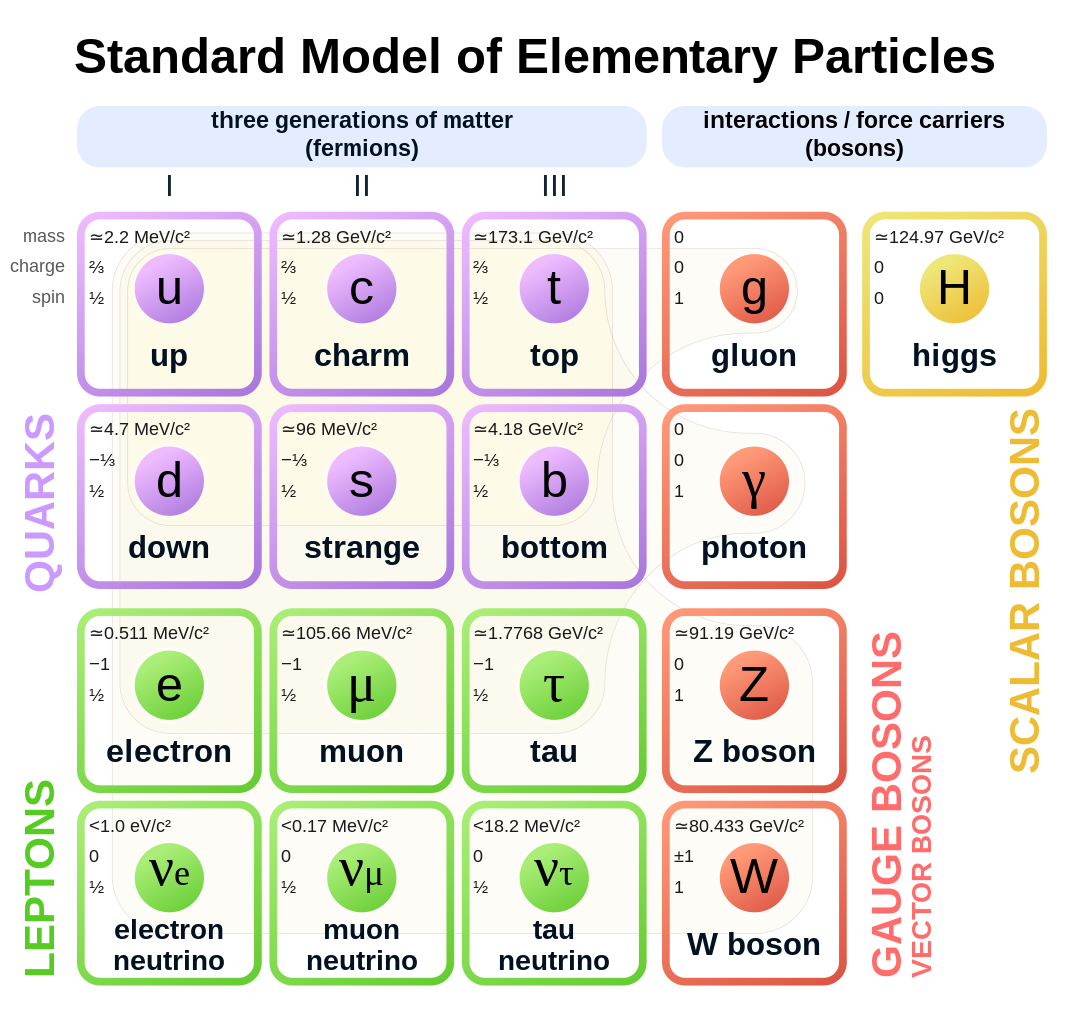
\includegraphics[width=0.7\textwidth]{figures/Standard_Model_of_Elementary_Particles.svg.png}
    \caption{The particles of the standard model of particle physics. There are 3 generations of quarks and leptons, which differ from previous generations only in their mass. Quarks are split into up-like quarks, with a $+\frac{2}{3}$ charge, and down-like quarks with a $1\frac{1}{3}$ charge. Leptons are split between charged leptons with charge $q=-1$ and neutrinos, which carry no electromagnetic or color charge, and are very light. There are 4 gauge bosons for the 3 fundametal forces which the standard model describes: the gluon ($g$) for the strong force, the photon ($\gamma$) for the electromagnetic force, and the W and Z bosons for the weak force. Additionally, there is the scalar higgs boson, which is responsible for the mechanism which gives other particles their mass.}
    \label{fig:StandardModelParticles}
\end{figure}


Quarks always form composite particles made up of either three quarks (baryons) or a quark-antiquark pair (mesons). %i know there are also pentaquarks, but they have nothing to do with this thesis and are therefore not mentioned
These two differ in the fact that baryons are fermions (half integer value spin) and mesons are bosons (integer value spin). The baryon number\footnote{The baryon number is a quantum number where baryons have 1 and antibaryons have -1.} is also conserved in all known reaction of the standard model, which means that the relative number of baryons-antibaryons remains constant. \\
It is important to note why quarks are never found individually. Quarks carry color charge, which is the charge of the strong force. The shape of the strong force does not allow for isolated color charges to exist, a principle called  color confinement. Unlike for example the electromagnetic force, which gets weaker as the distance between two particles grows, the strong force remains constant. The potential of the strong force can thus be phenomenologically described by the Cornell potential\cite{Strong_potential}, as given in equation \ref{eq:StrongPotential}:
\begin{equation}\label{eq:StrongPotential}
    V(r) = -\frac{4}{3}\frac{\alpha_s}{r}+\kappa r
\end{equation}
, where $\kappa$ is constant. The second term of equation \ref{eq:StrongPotential} dominates at large radii (>1 fm), and is thus responsible for the long distance behavior of the strong force. The energy stored in the field between two particles can be found by $\delta E(r_1-r_0) = V(r_1)-V(r_0) = \int_{r_0}^{r_1} \vec{F}.d\vec{r}$, i.e. the path integral of the force along the separation between the particles. If the force decreases enough\footnote{If the force decreases as 1/$r$, the integral of $\int_{x_0}^{\inf} \frac{1}{\vec{r} } .d\vec{r} \propto \mathrm{ln}(r)$ will go to infinity at infinite distances, therefore the force simply decreasing is not sufficient. However, if the force decreases as 1/$r^2$ -- as it does for the electromagnetic and gravitational forces -- the integral is finite at infinite distances.} as the distance grows, this allows potential energy to be stored in the field between two particles, without this energy becoming infinitely large at large distances. However, if the force remains constant even with larger distances, the energy stored in the field increases proportionally to the distance between particles. For the strong force, this gluon field between two particles which are being separated is often called a string. Eventually, enough energy is stored in the string that a new antiquark-quark pair can be created, isolating the color charges at each end of the string, thus splitting the string in two. The mount of energy stored in gluon strings is estimated to be roughly 1 GeV/fm\cite{}. This mechanism, which is shown in figure \ref{fig:IntroStringFragmentation}, is called string fragmentation, and is an intuitive explanation for why the color charges of the strong force cannot be isolated. \\

\begin{figure}[h!]
    \centering
    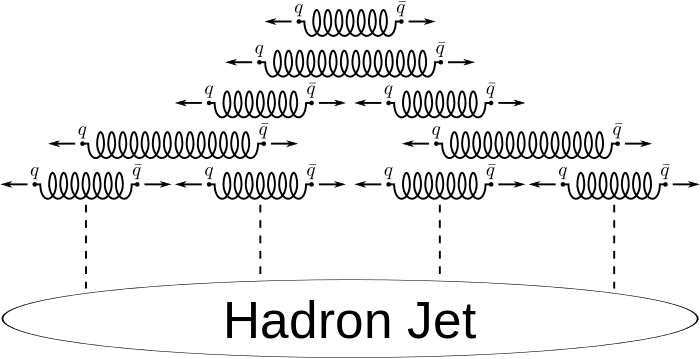
\includegraphics[width=\textwidth]{figures/String_fragmentation.png}
    \caption{Color confinement by string fragmentation. As the antiquark-quark pair moved away from each other, more and more energy is stored in the color flux tube between them. Eventually, there is sufficient energy to create a new quark-antiquark pair, and thus truncate the flux tube. This process continues until the (anti)quarks run out of sufficient energy to create new quark-antiquark pairs. The quarks can then hadronise. The figure is taken from \cite{StringFragmentationGraphic}.}
    \label{fig:IntroStringFragmentation}
\end{figure}




\subsubsection{Symmetries and symmetry breaking within the standard model}\label{sec:IntroSymmetries}
Symmetries are a fundamental aspect of the standard model. A symmetry can be defined as a global operation under which the laws of physics remain the same, and they can be deceptively powerful. In fact, something as fundamental as conservation of energy can be shown to be equivalent to a symmetry to translations in time. Other continuous symmetries such as spatial translation and spatial rotation give rise to conservation of momentum and angular momentum, respectively\footnote{The relations between physical symmetries and conservation laws was established by Noether's first theorem \cite{Noether1918}. }. But there are also symmetries which are not continuous, but discrete\footnote{In order to distinguish between a continous and discreet symmetry, consider the difference between spatial translations and spatial inversions. The first is an operation which moves a system to a different point in space. It does not matter if the movement happens by 1m or 1km, the symmetry should hold all the same and is thus considered continous. Meanwhile, spatial inversion inverts the direction of the axes, similar to how a mirror inverts one axis. This is not a continuous operation, since it is impossible to "half-mirror" an object.}. The standard model of particle physics contains three important and related discrete symmetries\cite{}. Under these symmetries, the laws of physics are expected to behave the same. C-symmetry, which stands for charge and represents replacing particles with their antiparticles. P-symmetry, which stands for parity symmetry, which represents spatial inversion along the 3 physical axes. And finally T-symmetry, which stands for time-inversion symmetry, which represents inversion of the direction of time. \\

They are called near symmetries, because each of them is individually broken within the standard model. A symmetry can be broken in two ways: explicitly or spontaneously. Explicit symmetry breaking is when the Lagrangian corresponding to an interaction does not itself respect the symmetry, while spontaneous symmetry breaking is when the Lagrangian respects the symmetry, but its ground state solution does not. The most famous individual violation is the breaking of P-symmetry of the weak force, which couples only to left-handed fermions and right-handed antifermions. In other words, a system of fermions and antifermions inverted under P-symmetry would no longer couple to the weak force, as the fermions are now right handed and the antifermions left handed. It is then obvious that replacing particles by their antiparticles would restore this symmetry. This combined symmetry is called CP-symmetry, and is thought to be respected by the strong and electromagnetic forces, however, there is a degree of CP violation in the mixing of different quark generations by means of the weak force, as described by the Cabbibo-Kobayashi-Masakawa (CKM) matrix. Introducing a complex phase in the quark mixing allows for the weak force to violate CP symmetry\cite{}. 

This can be exemplified by the following consideration. Consider a process $a \rightarrow b$, and the corresponding process with the antiparticles $\bar{a} \rightarrow \bar{b}$ and denote the amplitudes with $M$ and $\bar{M}$. By CP symmetry (i.e. before the violation), these numbers must be the same. We can separate them into a magnitude and a phase as $M = \bar{M} = |M|e^{i\theta}$. If there is a complex phase term introduced (for example by the CKM matrix) the amplitudes become $M = |M|e^{i\theta}e^{i\phi}$ and $\bar{M} = |M|e^{i\theta}e^{-i\phi}$. Since measurable rates are proportional to $|M|^2$, CP symmetry is still conserved. However, now consider the case where the reaction can take two different routes, $a \rightarrow 1 \rightarrow b$ and $a \rightarrow 2 \rightarrow b$ and the amplitudes become: $M = |M_1|e^{i\theta_1}e^{i\phi_1} + |M_2|e^{i\theta_2}e^{i\phi_2}$ and $\bar{M} = |M_1|e^{i\theta_1}e^{-i\phi_1} + |M_2|e^{i\theta_2}e^{-i\phi_2}$. This allows the calculation of the differences in amplitudes as $|M|^2 - |\bar{M}|^2 = -4|M_1||M_2|\mathrm{sin}(\theta_1 - \theta_2)\mathrm{cos}(\phi_1 - \phi_2)$. Thus, the introduction of a complex phase causes a violation between matter and antimatter. \\
CP violation was first observed in the decays of neutral Kaons\cite{CP_violations_early} in 1964, and was confirmed in 1999 \cite{CP_violations_proof}. Since then it has also been observed in the decays of $B$ and $D$ mesons \cite{CP_violation_B, CP_violation_D}. CP violation is also necessary (but not sufficient) in order to produce the matter-antimatter asymmetry, as is elaborated in section \ref{sec:IntroSakharovContidion}. Even though the CP symmetry is being violated, the combined CPT symmetry is expected to be conserved in all standard model processes\cite{}. 

Lastly, let us consider what is known as the strong CP problem. The QCD Lagrangian must include a CP violating term in order to account for the difference between the pion and $\eta$ masses \cite{tHooft}, which is characterised by a free parameter $0<\bar{\theta}<2\pi$. But by measurements of the neutron electric dipole moment it has been shown that $\bar{\theta} \lesssim 10^{-10}$. This represents a fine tuning problem: there must be a CP violating term in QCD, but it must also be set to be almost 0. So far, only one convincing solution has been introduced: the Peccei-Quinn (PQ) model. This model introduces a new global symmetry to the QCD Lagrangian, and a corresponding scalar field. This symmetry is then spontaneously broken at low energies, creating the axion\footnote{The name axion comes from a brand of laundry detergent, and was chosen because the axion "cleans up" the strong CP problem.}, a promising alternative dark matter model. For a more detailed mathematical description of the axion see \cite{axion_review}.


\subsection{Matter and antimatter in the universe}


\subsubsection{Origin of baryonic matter}
The majority of the baryonic matter we see in the universe was created within the first instances after the Big Bang. Initially, the universe was in a hot dense state, with temperatures much higher than the masses of the elementary particles. In fact, the temperature was so high that the higgs mechanism did not yet provide mass to particles\cite{Higgs_vev_highT} (T $\gtrsim 150$ GeV). During this time, quarks, leptons and bosons were in a thermodynamic equilibrium. As the universe underwent inflation, it became colder and colder, until eventually the higgs mechanism started to make particles massive\cite{Higgs_vev_highT} (see section \ref{sec:IntroBaryogenesisSM} for more details). This phase transition of the universe is one option for the source of the matter excess in the universe.
As the universe continued to evolve and temperatures cooled, quarks and gluons first formed a quark-gluon plasma -- a state of matter in which color charges can move freely\cite{} --  and eventually hadrons, which decay leaving only the most stable hadrons (protons and neutrons) behind. At this point about 1s had passed since the Big Bang. From about 10s to 20 minutes after the Big Bang, the temperatures enabled nuclear fusion. It was during this time that most of the deuterium, helium-4 and lithium in the universe were formed. \\

\begin{figure}
    \centering
    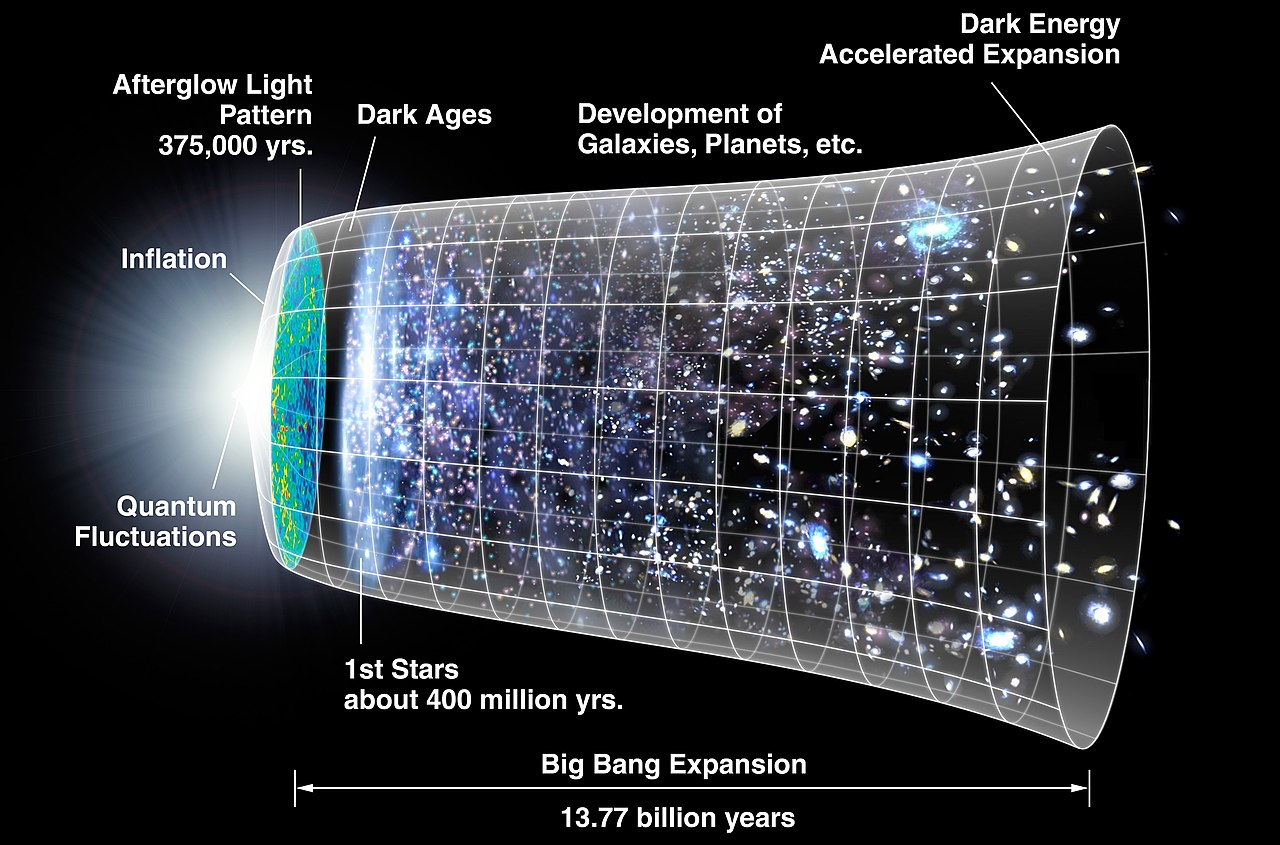
\includegraphics[width=\textwidth]{figures/CMB_Timeline300_no_WMAP.jpg}
    \caption{Timeline of the universe, starting from the Big Bang \cite{timelineOfTheUniverse}.}
    \label{fig:TimelineOfTheUniverse}
\end{figure}

The immediate period after the big bang shaped our universe in more ways than simply creating an excess of matter over antimatter. The gravitational collapse of dark matter during this time is thought to be responsible for the formation of galactic structures\cite{Ibarra_neutrinos}. The creation of nuclear matter determines the majority of the make up of the universe to this day. The timeline of the evolution of the universe is shown in figure \ref{fig:TimelineOfTheUniverse}.

\subsubsection{A matter dominated universe: antimatter-matter asymmetry}
To the best of our knowledge our universe is  entirely dominated by matter over antimatter. This observation is staggering, because in all the reactions we can observe in particle physics experiments near earth, whenever new matter is produced the same amount of antimatter is produced as well. So the a priori assumption is that the universe houses as much antimatter as it does matter. And at first glance, this doesn't seem to impose any impossible constraints, as from a distance matter and antimatter are indistinguishable\footnote{This means to say that matter atoms would produce the same spectral lines as antimatter atoms, and undergo the same fusion reactions we see in stars.}. So while our solar system might be made of matter, what is to keep other solar systems, or even other galaxies from being made of antimatter? The issue arises when we look at the surroundings of solar systems or galaxies. Interstellar/intergalactic space is not completely empty, but populated at very low densities by protons and helium-4 from surrounding stars/galaxies. We know the density of protons in these regions to be about $n_\mathrm{H} \approx 1$ cm$^{-3}$ for interstellar space\cite{}, and $n_\mathrm{H} \approx 1$ m$^{-3}$ for intergalactic space \cite{}. And when a matter dominated region and an antimatter dominated region are next to each other, then in this vast space of low density matter, plenty of annihilations would occur. These annihilations would produce distinctive signals in gamma ray searches, due to high energy photons emitted from $e^+e^-$ annihilations or from the decay of $\pi^0$s produced in $\mathrm{p}\overline{\mathrm{p}}$ annihilations\cite{Schönfelder1989}. The lack of any such signals places stringent limits on any large areas of antimatter within the observable universe, and leads us to believe that our universe is indeed dominated by matter. The source of this matter-antimatter asymmetry is one of the big remaining mysteries of physics.  \\

It isn't known exactly how the different populations of matter and antimatter came to be. Perhaps only a minute difference between the two caused a tiny fraction more matter to be produced than antimatter. And since the majority of both annihilated, what we see today might by this tiny leftover fraction. For this reason, searches for differences between matter particles and their antimatter counterparts are looking to find even the tiniest discrepancy between the two\cite{}. 

\subsubsection{Sakharov condition}\label{sec:IntroSakharovContidion}
Given the a priori assumption that the same amount of matter and antimatter would be produced, it is necessary to clarify the conditions under which this could be altered. In \cite{Sakharov:1967dj}, the necessary conditions for the creation of a baryon excess were shown to be:
\begin{itemize}
    \item Some interactions of elementary particles must violate baryon number conservation, since the net baryon number of the universe must change over time
    \item C and CP must be violated so that there is no equality in the forward and backward rates of the baryon number violating processes. 
    \item The net flux must be created in out-of-equilibrium conditions, since otherwise CPT symmetry would assure compensation of the effect. 
\end{itemize}

The first condition is trivial. The second condition means that there must be a reaction which differentiates between the matter and antimatter, in order to give rise to a process which would preferably create baryons over antibaryons. The third condition requires some more explanation. It is based on the fact that we believe the CPT symmetry to be exact. Therefore, there must be a process which only happens in one direction in time. This cannot occur in an equilibrium condition, since in equilibrium all reactions occur in both the forward and backward directions. Therefore, it must be a reaction linked to out-of-equilibrium processes. 


\subsubsection{Baryogenesis within the standard model}\label{sec:IntroBaryogenesisSM}
It is possible to account for the matter-antimatter asymmetry in the universe through standard model processes. One such process was outlined in \cite{Bubbles_asymmetry}. The main arguments of this paper are reproduced here, to exemplify how the Sakharov condition above can be applied. \\

The main idea of the mechanism is threefold: i) the existence of a first order phase transition as the universe cools below the electroweak phase transition. The phase transition satisfies the out-of-equilibrium part of the Sakharov conditions. ii) quarks and antiquarks scattering of the phase boundary in an asymmetric fashion, due to CP-violating effects. This results in a net baryon flux through the phase boundary. And iii), the excess antiquarks in the hot medium are removed by an effect which does not conserve baryon number, before the phase transition is complete in the entire universe. \\
In the standard model, particles get their mass by their Yukawa coupling to the higgs vacuum expectation value\cite{SANTAMARIA199390}. The vacuum expectation value of the higgs field vanishes at temperatures above the electroweak phase transition, such as were present during the early universe\cite{Higgs_vev_highT}. If this phase transition is treated as a first order phase transition, with bubbles of the colder phase forming out of the hot medium, then the vacuum expectation value of the higgs will change while crossing the phase boundary. This will change the masses of fermions as they move across this phase boundary, which thus acts as a potential barrier. This causes both quarks and antiquarks to scatter from this barrier. However, due to the CP-violating nature of the weak interaction, the transmission through the barrier can be different for quarks and antiquarks, resulting in a baryon flux through the phase boundary. Excess antiquarks in the medium are then removed by sphalerons. A sphaleron is a solution to the electroweak field equations, geometrically represented by a saddle point which connects a 3 baryon system to a 3 antilepton system\footnote{And equivalently 3 antibaryons to 3 leptons.}\cite{Phong_2020}. Sphaleron effects are expected to be frozen out below about 10 TeV. Since the temperature is higher on one side of the phase transition than the other, the baryon number symmetry violating process is hypothesised to occur only on the hot side, and thus leave a net baryon number.  \\

While sphalerons are currently hypothetical, it is expected that the high luminosity upgrade of the LHC will be able to start the experimental search for sphalerons \cite{Papaefstathiou_2019}.


\subsection{Antimatter-matter annihilations}
The lightest quarks -- $u$ and $d$ -- make up normal nuclear matter, i.e. protons $uud$ and neutrons $udd$, which are the two lightest baryons with masses of 938 MeV/$c^2$ and 939 MeV/$c^2$, respectively. Since the proton is the lightest baryon, and the baryon number must be conserved, any reaction of the proton with other matter must leave an intact proton at the end, thus never making the energy stored in the proton's mass available to create new particles. When baryons interact with their antibaryons, they annihilate, releasing their entire mass as available energy to create new particles. This is because by definition, the total baryon number of such a reaction is 0. The same is true for the annihilations of leptons and lepton number conservation, and for the conservation of electric charge in the annihilations of leptons and baryons. In principle, if a quantum number is antisymmetric under the C symmetry, it will be conserved by construction in antimatter-matter annihilation events and thus will never limit the available phase space of reactions. \\

\subsubsection{Annihilation of $q\bar{q}$ and $l\bar{l}$ pairs}

It is simplest to start with the Feynman diagrams for the annihilations of elementary quarks and leptons. The lowest order diagrams are given in figure \ref{fig:annihilationsFeynmanElementary}. Their relative contribution is proportional to the force's interaction strength to the exponent of the number of vertices, so $\alpha$ for the electromagnetic force, $\alpha_w$ for the weak force and $\alpha_s$ for the strong force. At low energies, the three parameters have an ordering $\alpha_s$>>$\alpha$>>$\alpha_w$\footnote{The couplings depend on the energy scale, as all of them are running coupling constants. At high energies, the weak force is actually stronger than the electromagnetic force. This difference is due to the mass of the weak bosons.}. Essentially, quark and leptons can annihilate with their antiparticles through electromagnetic and weak channels, which can also convert from quarks to leptons and vice versa. Quarks can additionally annihilate via a gluon into either another quark-antiquark pair or into hadron jets. For quarks, annihilation through the strong force should outweigh annihilation through the electromagnetic force by a factor $\alpha_s^2/\alpha^2 >>1$, which means that the strong channel should dominate. 

\begin{figure}
    \centering
    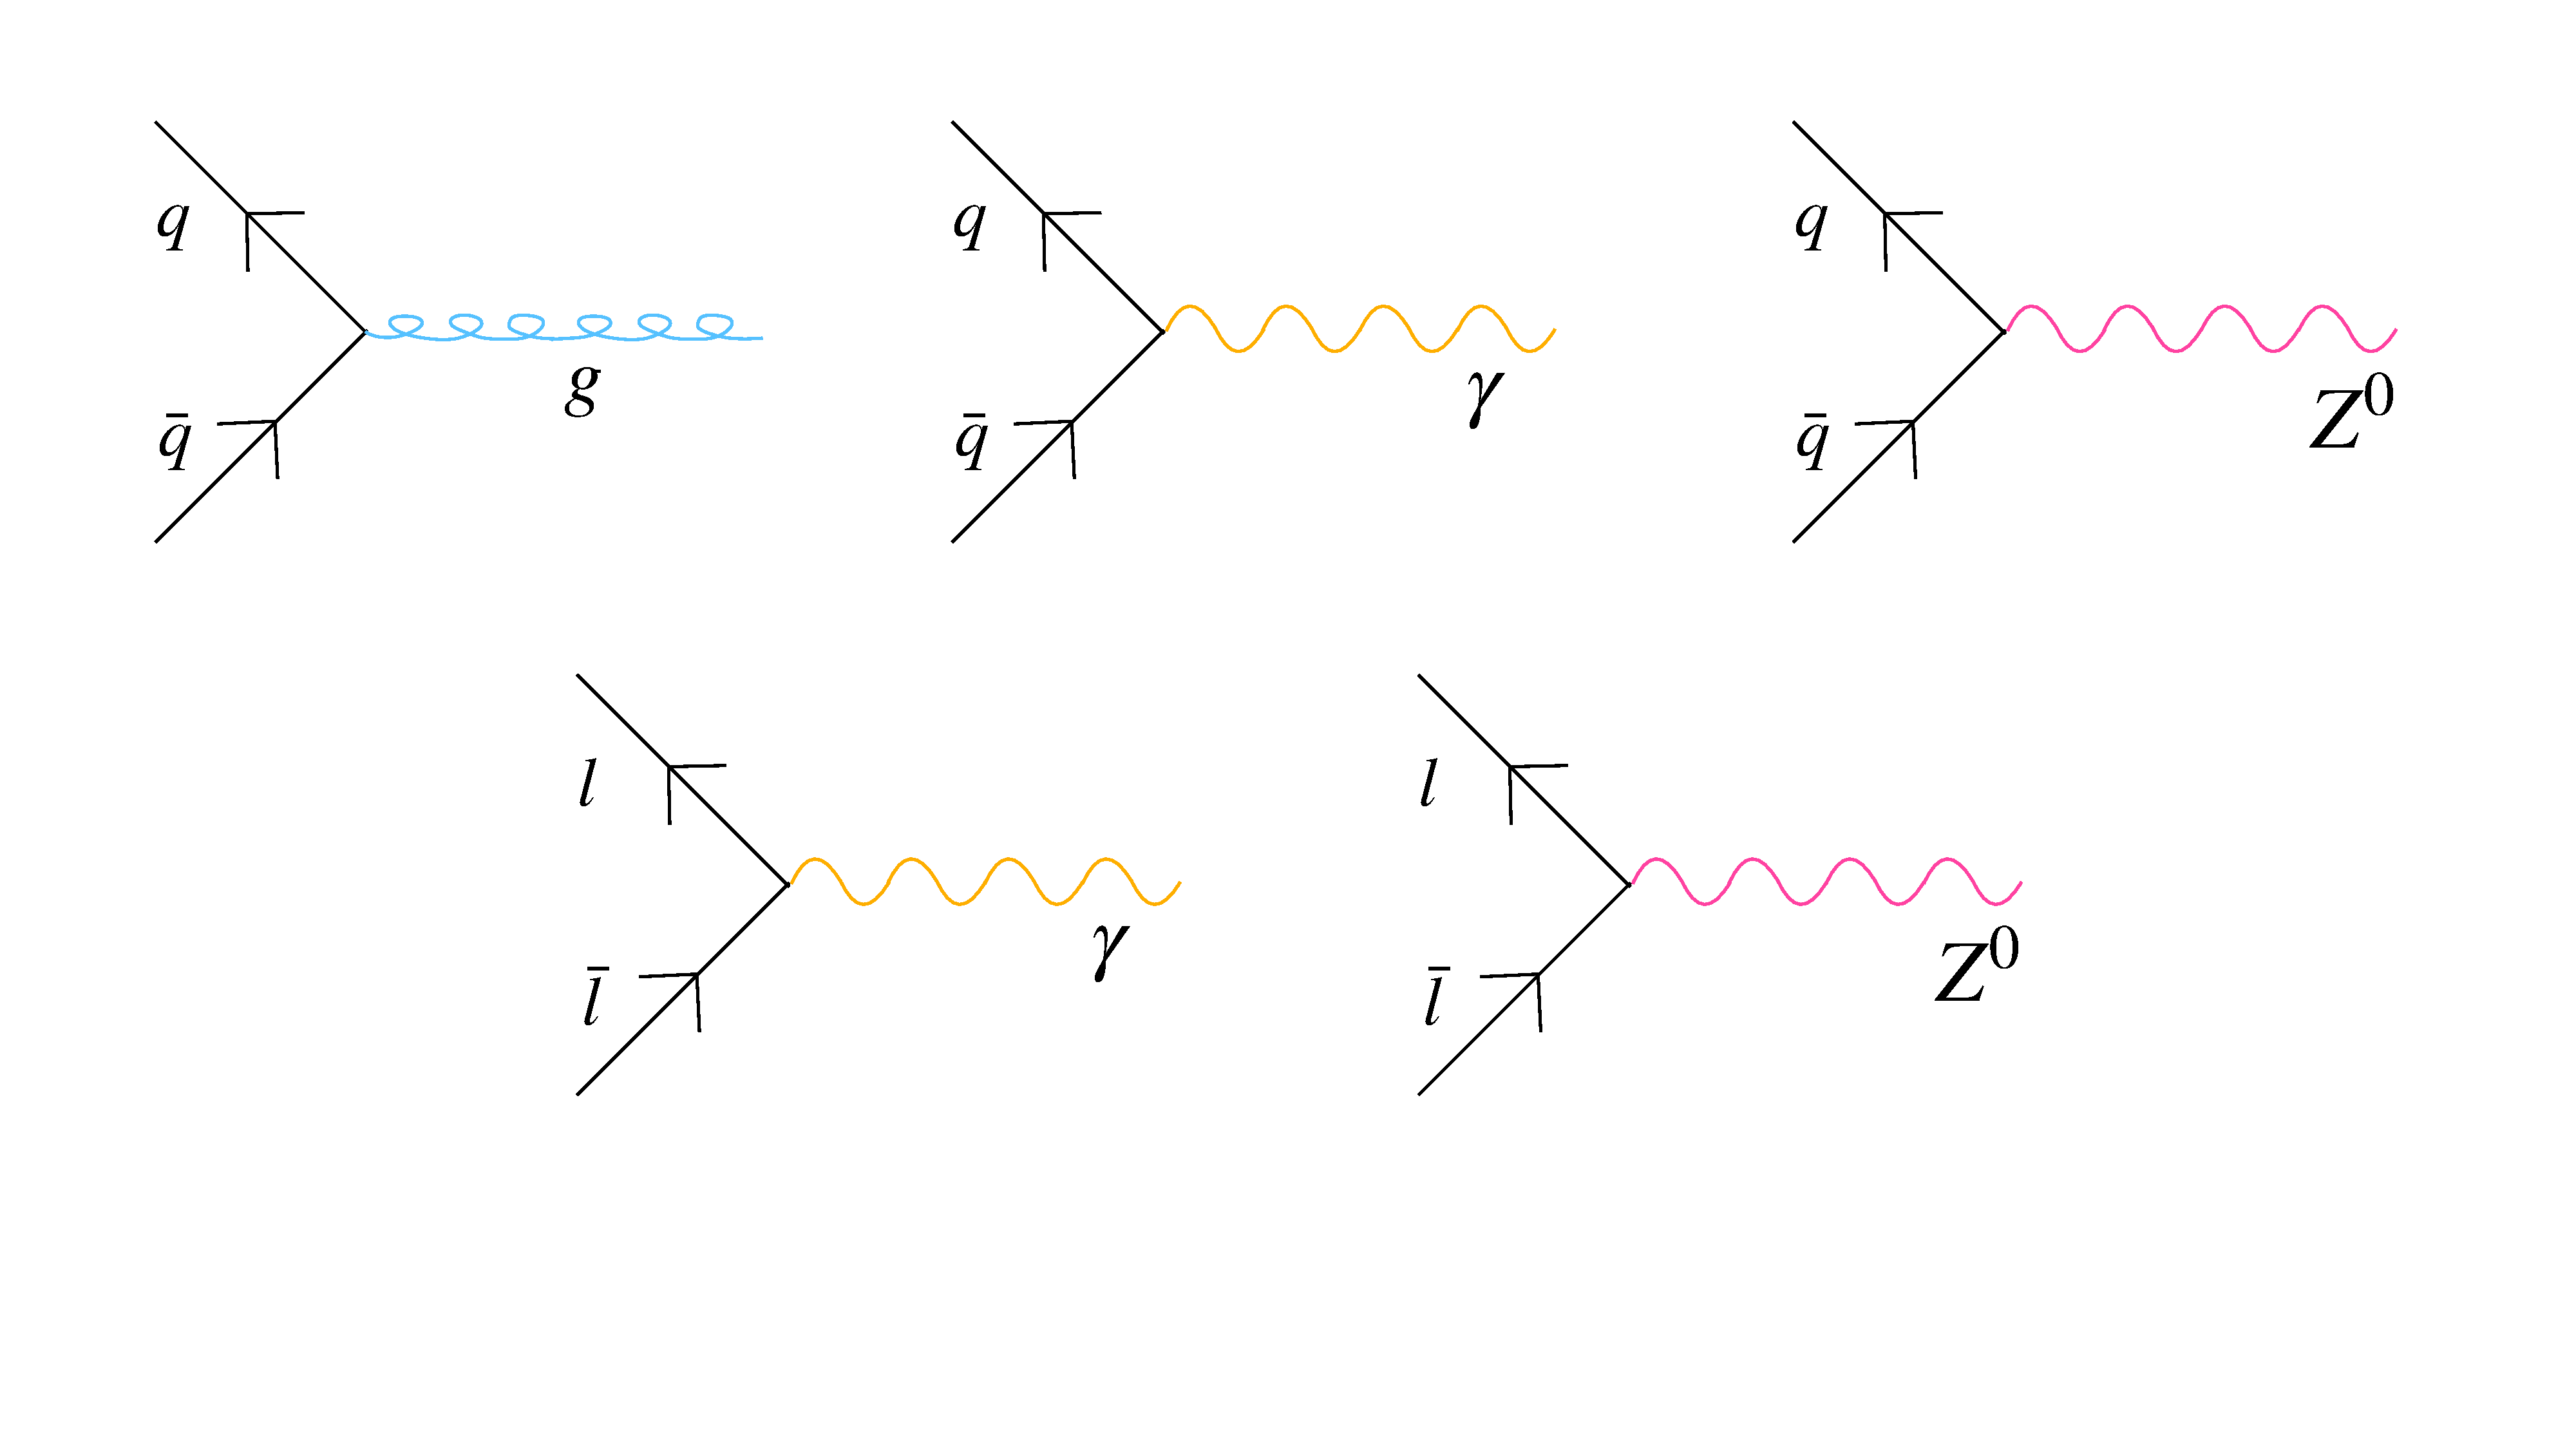
\includegraphics[width=0.9\textwidth]{figures/Annihilation_Feynman_diagram.pdf}
    \caption{First order Feynman diagrams showing the annihilations of elementary particles. Top row: quark-antiquark annihilation through the strong (left), electromagnetic (middle) and weak (right) force. Bottom row: lepton-antilepton annihilation through the electromagnetic (left) and weak (right) force.}
    \label{fig:annihilationsFeynmanElementary}
\end{figure}

\subsubsection{Antiproton-proton annihilations}
It is important to note at the start of this chapter that there is currently no theory or even model which can describe the available data for antiproton-proton annihilations, or offer up an explanation for the underlying mechanism\cite{antiproton_cross_sections_review}. This is in stark contrast to quark-antiquark annihilation, which is just a first order QCD process. In this section I shall attempt to give an overview of the difficulties in describing this process, and thereby offer up a qualitative picture of the possible annihilation mechanisms.\\

It is tempting to assume that in order to scale up an annihilation event, one might just be able to scale up the single Feynman diagrams for quark-antiquark annihilation in order to get a description for antiproton-proton annihilation. However, the picture is far more complicated. This can be intuitively understood by the fact that (anti)protons are made up of 3 valence (anti)quarks, but in the annihilation of (anti)proton pair, some of their valence (anti)quarks may well survive. In fact, consider the following reaction $\matrm{p\bar{p}} \rightarrow 3 \mathrm{M}$, where M denotes a meson. This reaction can occur by simply rearranging the quark content of the proton and antiproton, which is illustrated in figure \ref{fig:Quark_Rearrangement}. Such a rearranging of the quarks can happen if the quarks can feel each others strong potential, which can be mediated through pion exchange. This can be seen as equivalent to nucleon-nucleon interactions through pion exchange, at distances beyond the confines of color confinement. This effectively allows the potential for quark rearranging to be felt at further distances than the potential for quark-antiquark annihilation. The annihilation potential between an antiproton-proton pair therefore can have a long range ( $\gtrsim 1$ fm ) and a short range ($\lesssim 1$ fm) term, where the long range term is dominated by the rearrangement of quarks and antiquarks into mesons, and the short range term is dominated by quark-antiquark annihilation. The common notation of these processes is $An$ and $Rn$ for annihilation ($A$) and rearrangement ($R$) into $n$ mesons.\\

\begin{figure}[h!]
    \centering
    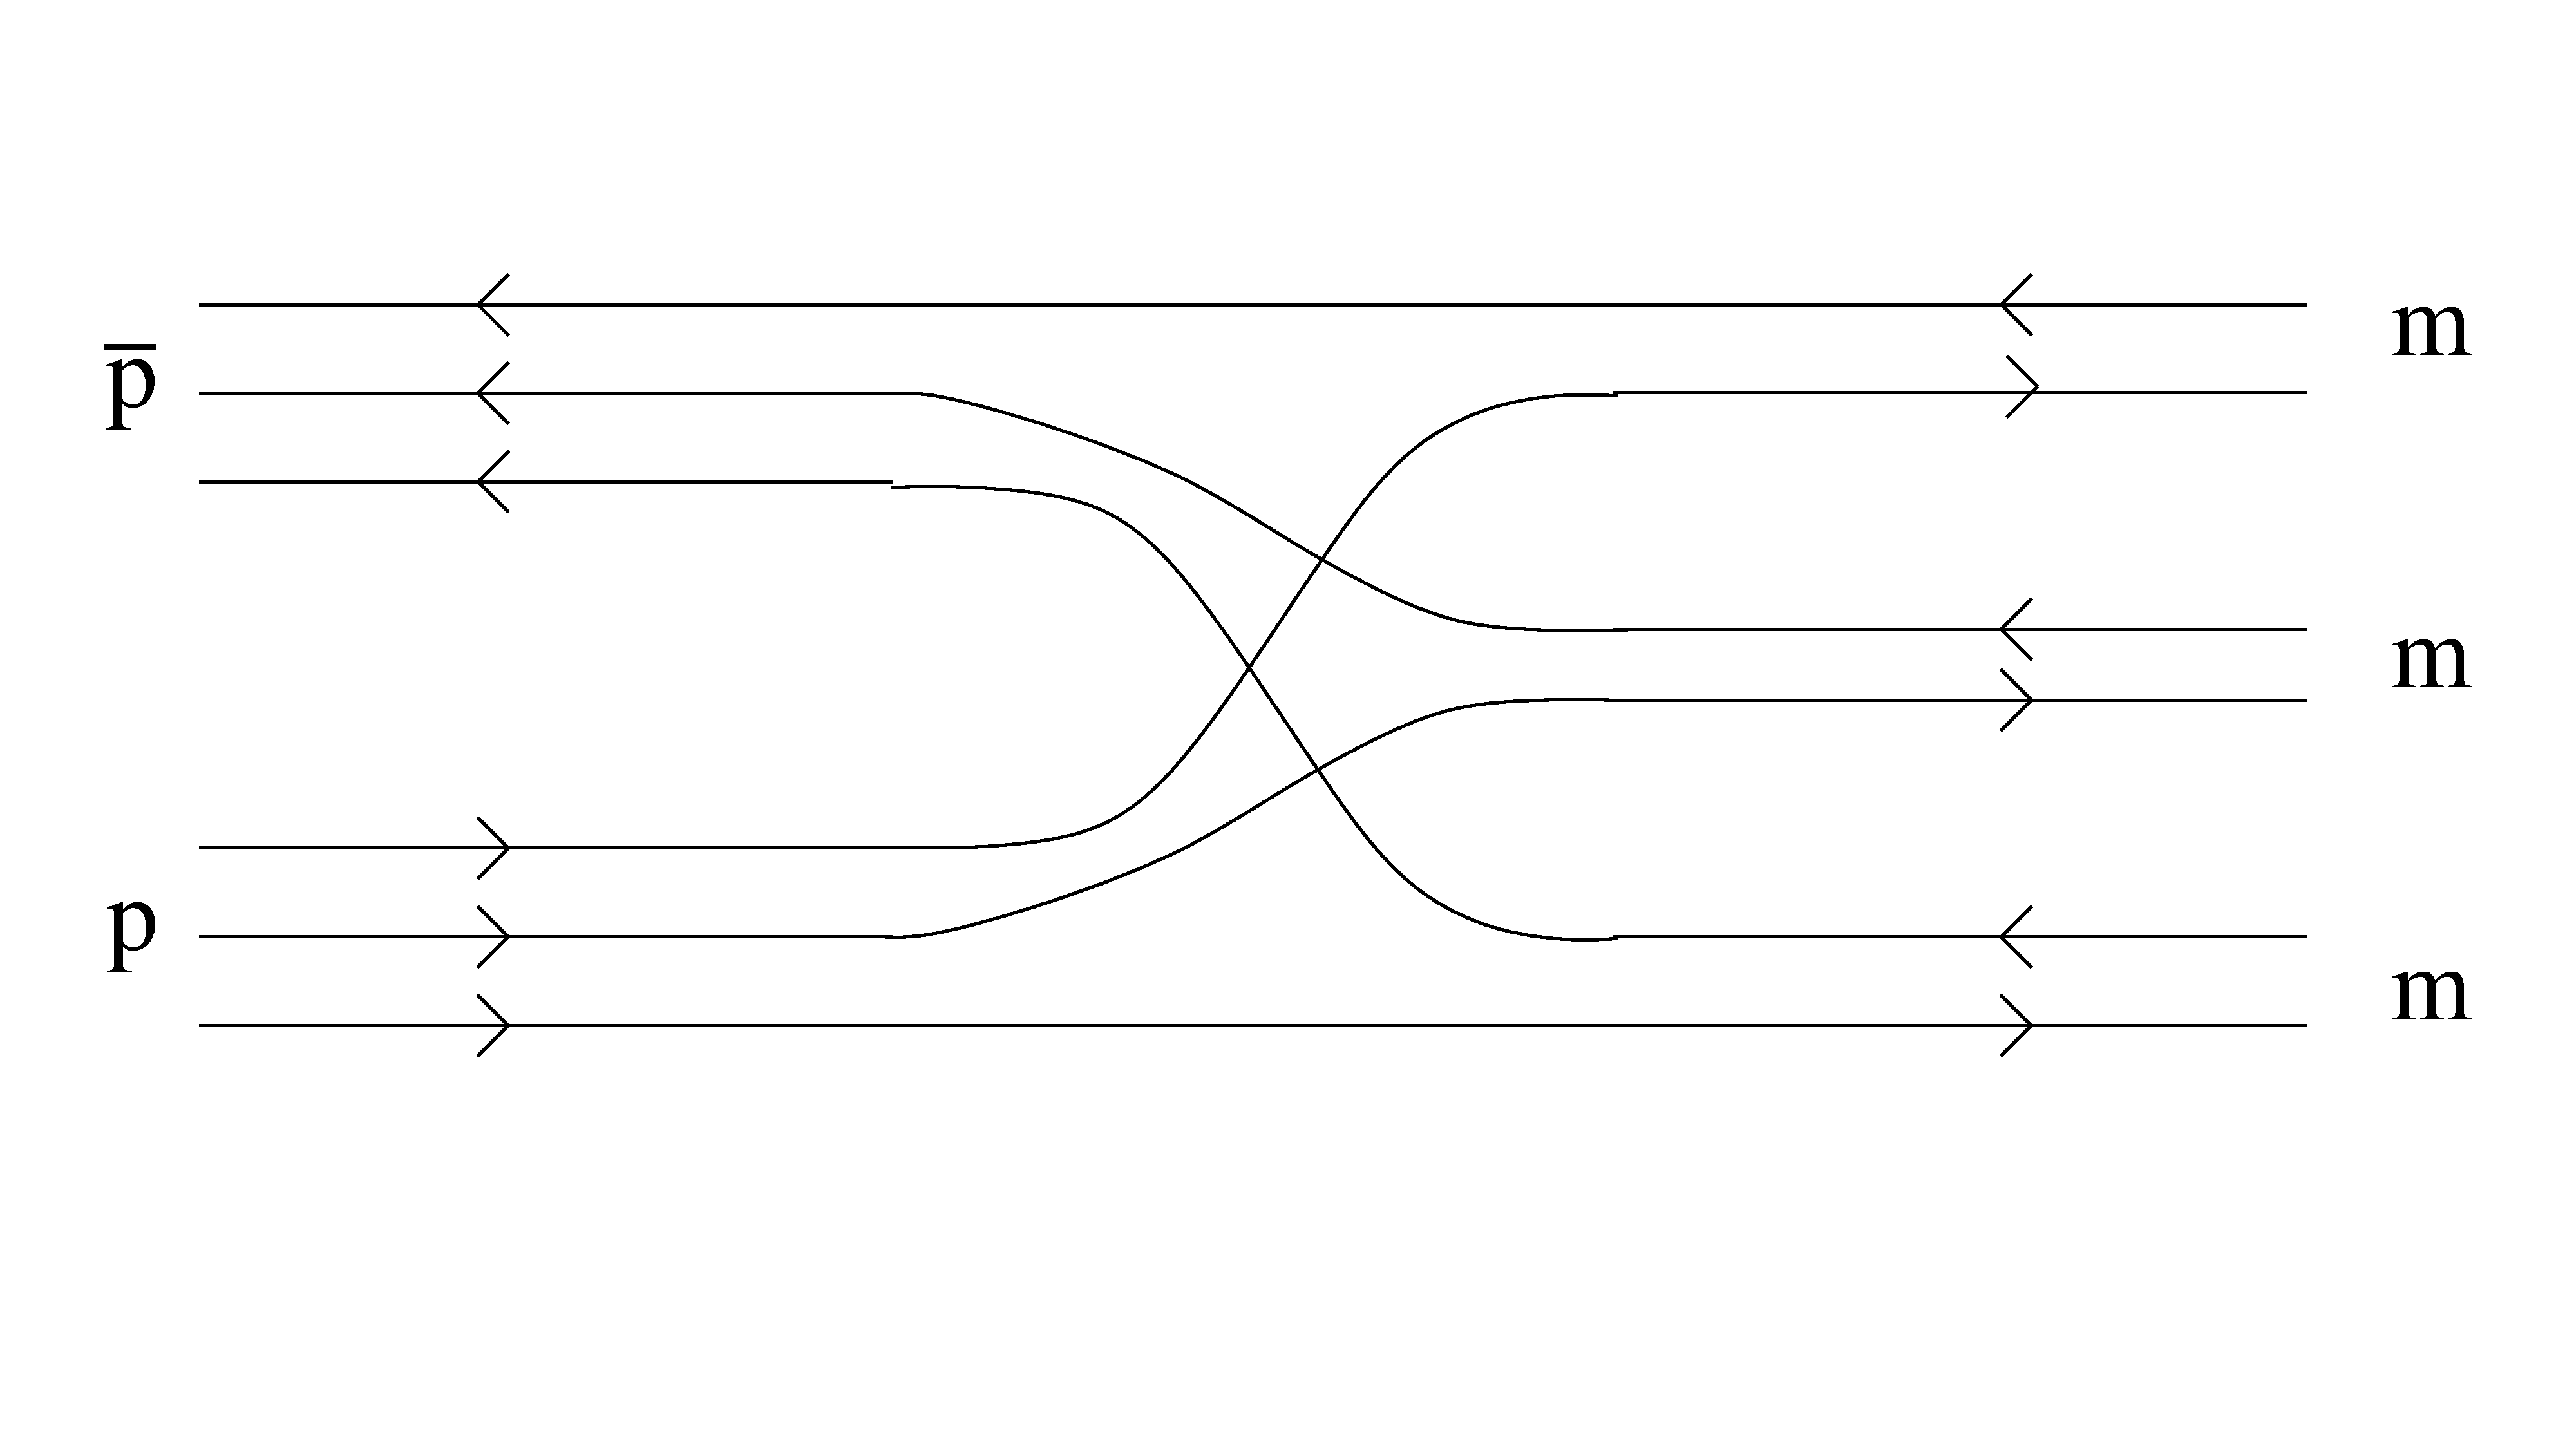
\includegraphics[width=0.9\textwidth]{figures/quark_rearrangment.pdf}
    \caption{Schematic of $\matrm{p\bar{p}}$ annihilation into 3 mesons, done by rearranging the valence quarks but without annihilating any quark-antiquark pair.}
    \label{fig:Quark_Rearrangement}
\end{figure}

%This is further complicated by the fact that due to the release of significant energy, multiple further mesons may be formed by strong fragmentation in either of these reactions. 
One important observable to distinguish between these two different annihilation mechanisms is the production of strangeness, i.e. by the reaction $\mathrm{p\bar{p}} \rightarrow 2\mathrm{K}+ X\mathrm{M}$. This reaction cannot occur with a simple rearrangement of quarks\footnote{Neglecting quark-antiquark creation by string fragmentation.}, as a new $s\bar{s}$ pair has to be created. If antiproton-proton annihilation would be dominated by the rearrangement of quarks, we would expect to see almost no produced kaons, while if the quark annihilation channel would dominate, we would expect to produce Kaons almost as much as pions. In fact we observe about 5\% of final states which include kaons\cite{antiproton_cross_sections_review, hidden_Strangeness}, suggesting that the truth lies somewhere in between the two models. \\

Given these considerations, the antiproton-proton annihilation cannot easily be described by perturbative QCD, and we are still missing an effective model capable of explaining the data. This is what makes an effective model of this interaction so difficult. Instead, an empirical parameterization is commonly used to describe the antiproton-proton inelastic cross section. A description accurately fitting the available data has been proposed by Tan et al. \cite{Tan_1983}, and is reproduced in equation \ref{eq:Talpbarpxs}, where $T_\bar{p}$ is the antiproton kinetic energy in the proton rest frame. 
%

\begin{equation}\label{eq:Talpbarpxs}
    \sigma_\mathrm{inel}^{p\bar{p}} = 24.7 (1 + 0.584T_{\bar{p}}^-0.115 + 0.856 T_{\bar{p}}^{-0.566}) \mathrm{mb}
\end{equation}

Another description -- which is implemented in the propagation code Geant4 -- is based on attempting to assign cross sections to each individual process which might occur and is explained in \cite{antiproton_dynamics_CERN}. In their model, they split the antiproton-proton annihilation into the sub processes laid out in figure \ref{fig:antiproton_annihilation_channels}. The momentum dependence of these processes is given by Regge theory \cite{antiproton_dynamics_2, antiproton_dynamics_CERN, Regge1959}. This method works for determining the cross sections into particular channels, which is necessary for an accurate description of particle propagation, as is shown in figure \ref{fig:pbar_p_xs_data_comp}. However, the description does not manage to describe experimental data better than within a factor 2. This highlights the difficulties in accurately describing the inelastic cross section of antiproton-proton annihilations.

\begin{figure}
    \centering
    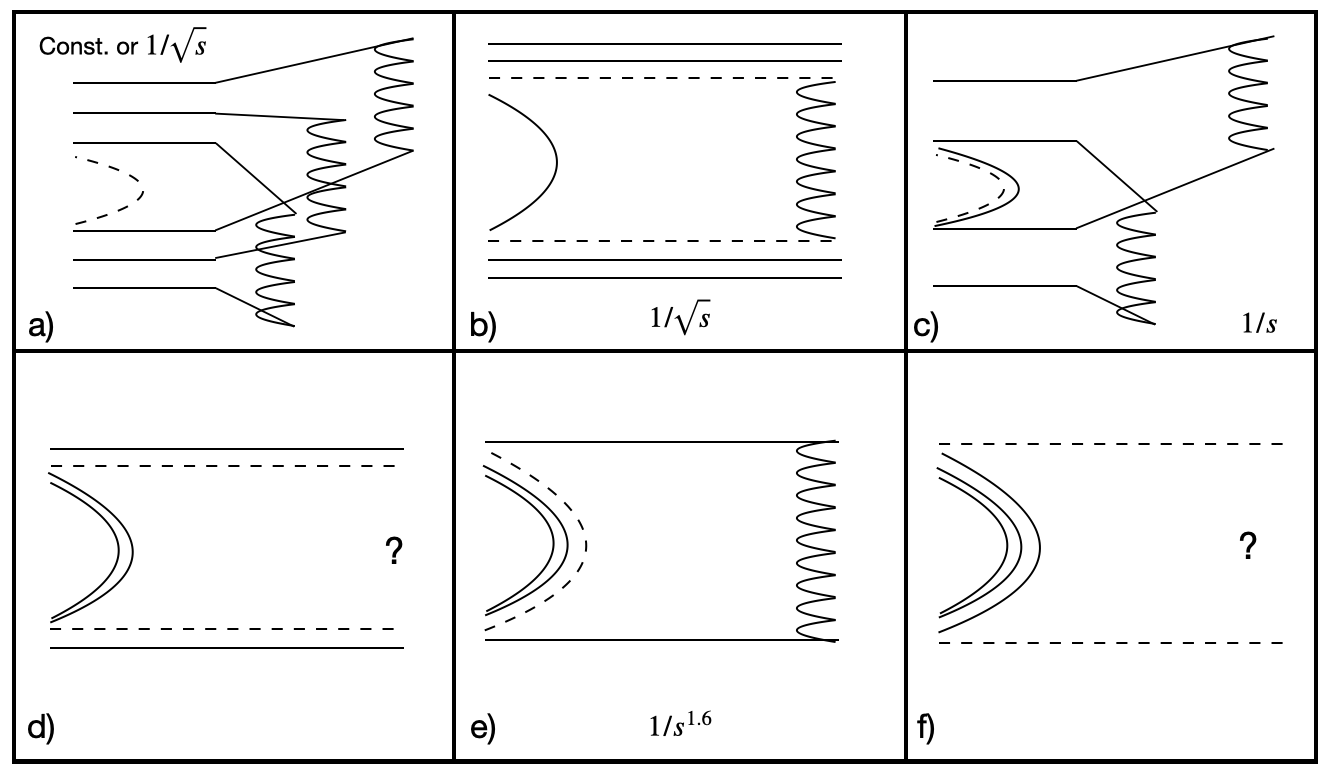
\includegraphics[width=0.6\textwidth]{figures/pbar_p_annihilation_channels.png}
    \caption{Annihilation channels for antiproton-proton annihilation. The solid lines represent quarks and the dashed lines represent a gluonic string (which can then decay via string fragmentation, as shown in figure \ref{fig:IntroStringFragmentation}). Curled lines represent a $\bar{q}q$ annihilation. The diagrams thus represent: a) 3 antiquark-quark annihilations; b) a single antiquark-quark annihilation into 2 mesons and a gluon string; c) Corresponds to a quark-antiquark and string annihilation, with the creation of 2 quark-antiquark strings. Diagrams e) and f) can produce exotic mesons. Figure taken from \cite{antiproton_dynamics_2}. \textit{This is unfortunately the highest quality figure available for this. I am planning to remake this figure in higher resolution.}}
    \label{fig:antiproton_annihilation_channels}
\end{figure}
\begin{figure}[h!]
    \centering
    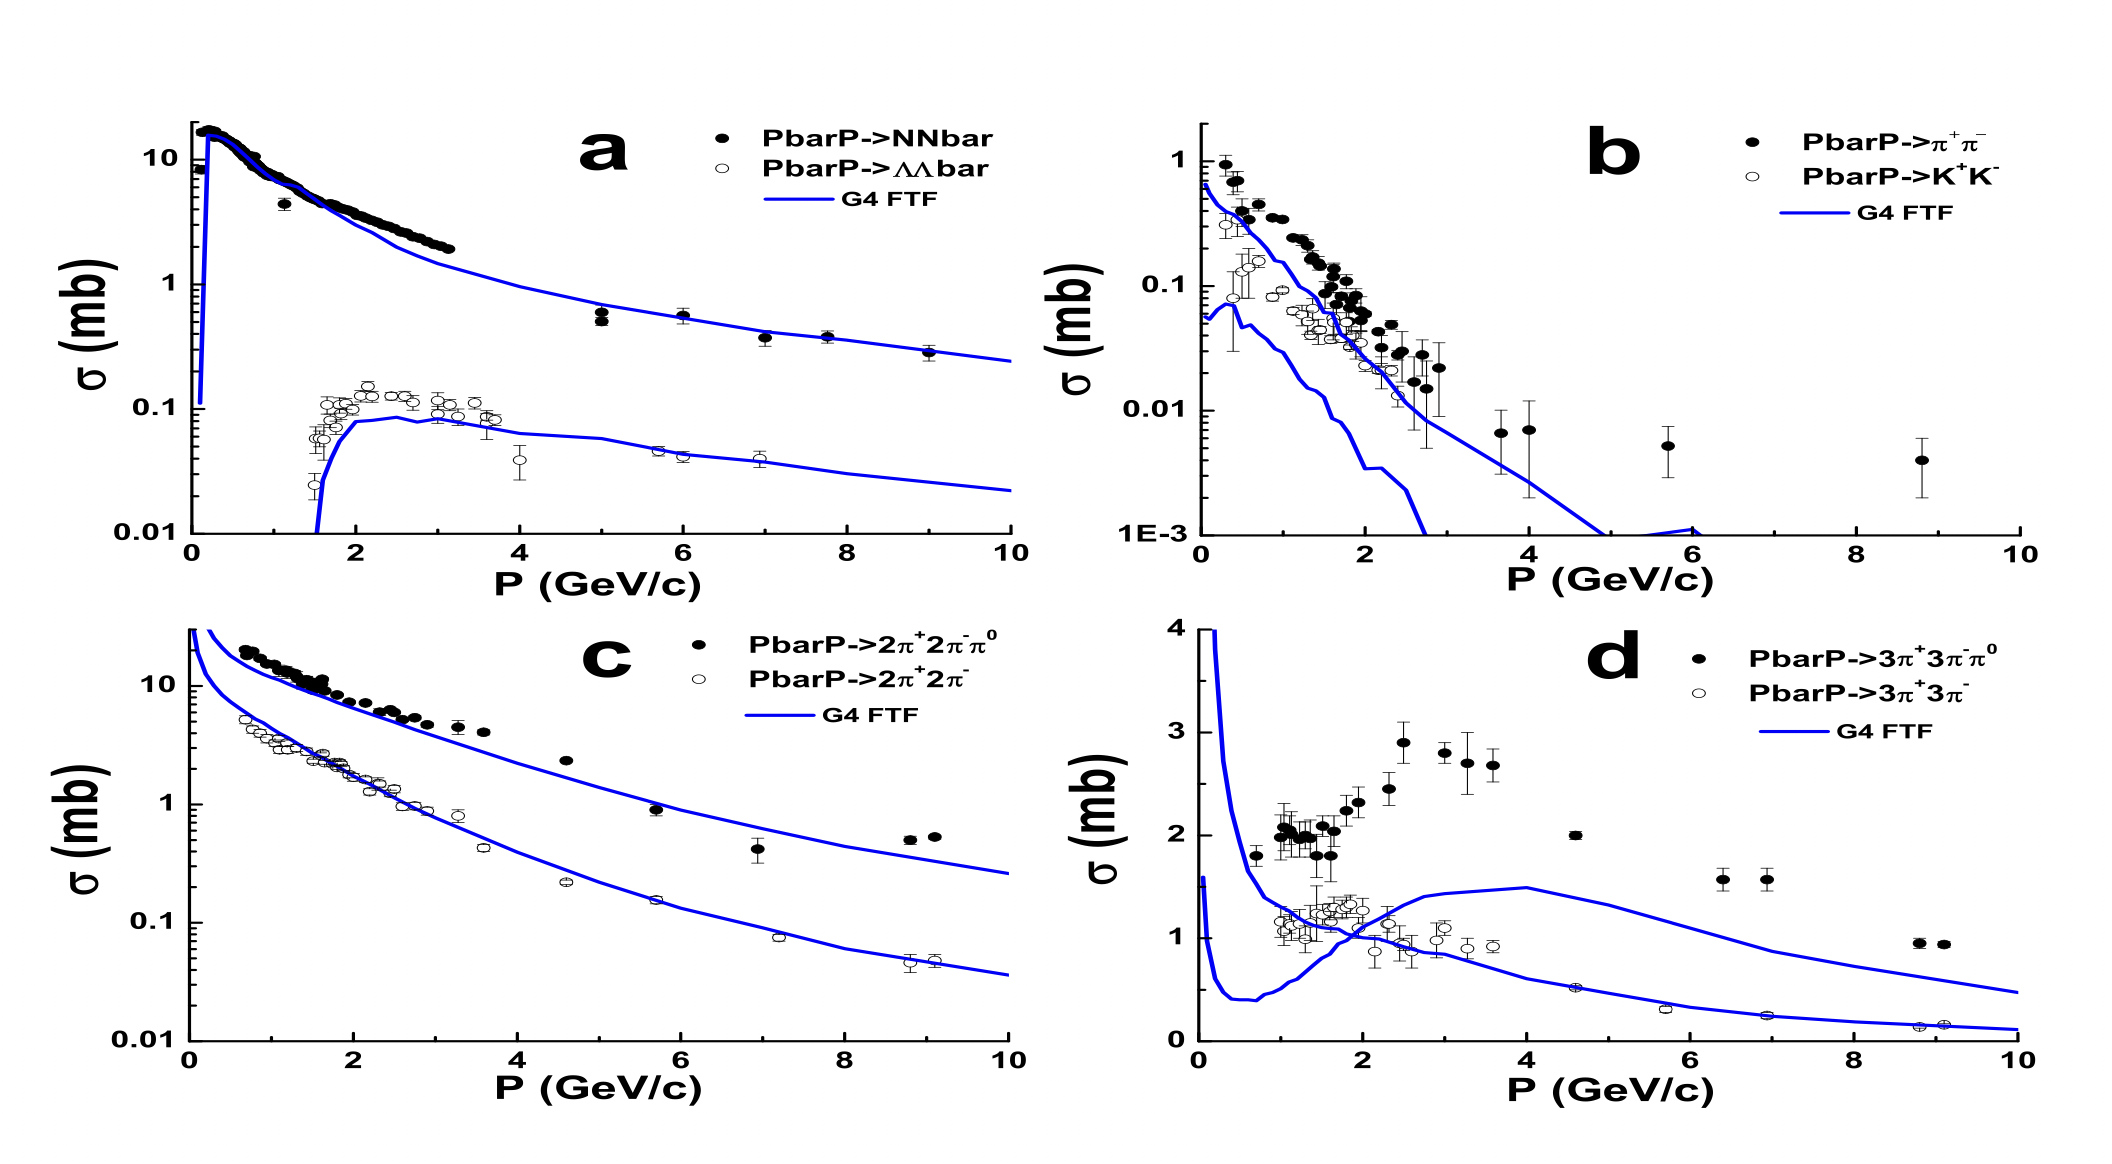
\includegraphics[width=\textwidth]{figures/Geant4_pbar_inel.png}
    \caption{A comparison of antiproton-proton inelastic cross section data with the model used in Geant4 \cite{antiproton_dynamics_CERN}. Points are experimental data as described in \cite{pbar_data}, the blue line represents the model.}
    \label{fig:pbar_p_xs_data_comp}
\end{figure}
An overview of available data on the antiproton-proton annihilation data is given in \cite{hidden_Strangeness, antiproton_physics_data, pbar_data}.



\subsubsection{Antiproton-nucleus annihilation: the Glauber model}
In the previous section it has been established that while the antiproton-proton inelastic cross section has been well measured, a theoretical description is still lacking. In this section we therefore focus on the experimental results for antiproton-matter annihilations, and how we can use them to infer something about the underlying annihilation mechanism. \\

When moving from antiproton-proton to antiproton-nucleus annihilations, several new effects come into play. The question is if only one nucleon in the nucleus interacts in the initial annihilation, and then how the antinucleus acts after the annihilation occurs. Thankfully, while those points certainly raise additional difficulties in finding a theoretical description, we can benefit from plentiful measurements of antiproton absorption on matter. These are parameterised according to the Glauber model \cite{Glauber_original, glauber_model_geant4_scaling, Antinucleus-nucleus_Geant4}. The Glauber model parameterises the inelastic cross section of antiprotons on nuclei as a geometric scaling of the antiproton-proton cross section, according to equation \ref{eq:Glauber_singleA}, where $R_A$ is a free parameter which can be roughly understood as the target nucleus' radius, and characterised as $R_A = r_0 A^{1/3}f(A)$. $r_0=1.1$ fm, and $0.8<f(A)<1.1$ is a correction factor as a function of $A$. $h$ denotes the hadron in question, $A$ is the mass number of the target nucleus and $\sigma_{hN}^{tot}$ is the total antiproton-nucleon cross section. 

\begin{equation}\label{eq:Glauber_singleA}
    \sigma_{hA}^{in} = \pi R_A^2 \mathrm{ln}\left[ 1+\frac{A\sigma_{hN}^{tot}}{\pi R_A^2}\right]
\end{equation}

\begin{figure}
    \centering
    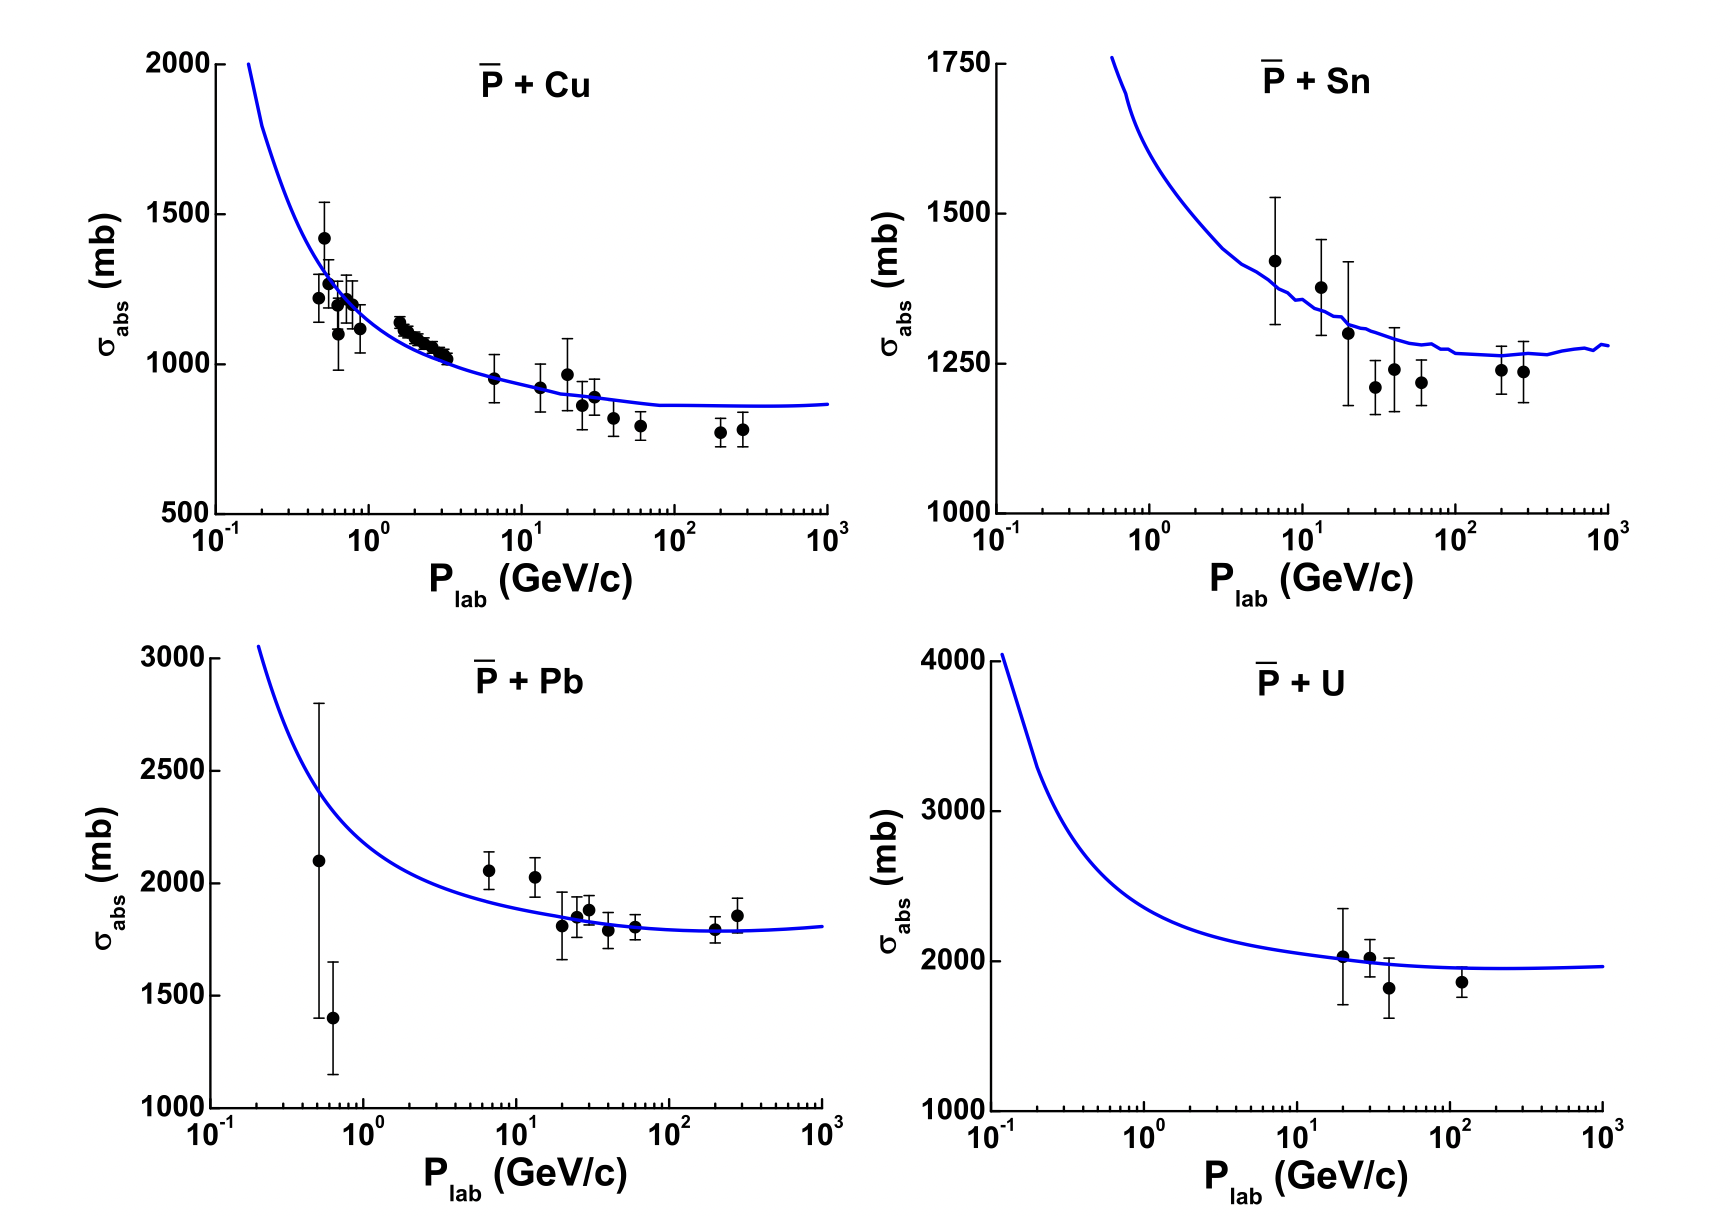
\includegraphics[width=0.9\textwidth]{figures/pbar_annihilation_diff_materials.png}
    \caption{Antiproton-nucleus annihilation for different materials, taken from \cite{Antinucleus-nucleus_Geant4}.}
    \label{fig:pbar_diff_materials}
\end{figure}


\subsubsection{Antinuclei-matter annihilations: the Glauber model and geometric scaling}\label{sec:IntroGlauber}
Having established the details of the antiproton inelastic cross section, we can now start to consider the process of antinuclei annihilation. All the considerations made for the antiproton inelastic cross section still hold true, but additionally there is also the potential between the antinucleons to consider. This means that one not only has to consider the breakup of the matter nucleus, but also the breakup of the antimatter nucleus, leaving a smaller antinucleus behind. This has been observed for antideuterons in the reaction $\overline{\mathrm{d}} + A \rightarrow \overline{\mathrm{p}}+X$\cite{Denisov:1971im, Binon:1970yu}. However, it is not clear if the antiproton which was measured survived the initial collision or if it was created from the annihilation of the antideuteron.\\

In order to scale up the cross sections from antiproton-nucleus to antinucleus-nucleus annihilations, we can also employ the Glauber model. The full mathematical treatment can be found in \cite{Uzhinsky:2011zz}, however, due to the computational effort required to do real time Glauber calculations, Geant4 uses a parameterization to approximate the result of Glauber calculations. This parameterization is based on extending \ref{eq:Glauber_singleA} to light antinuclei, according to equation \ref{eq:Glauber_multA}, where $B$ is the mass number of the antinucleus. 

\begin{equation}\label{eq:Glauber_multA}
     \sigma_{BA}^{in} = \pi(R_A^2+R_B^2) \mathrm{ln}\left[ 1+\frac{BA\sigma_{hN}^{tot}}{\pi ( R_A^2 + R_B^2)}\right]
\end{equation}

$R_A$ is then used as a fit parameter to tune the simplification to the expected value of full Glauber calculations. The form of $R_A$ is given by equation \ref{eq:RA}:

\begin{equation}\label{eq:RA}
    R_A = c_1 A^{0.21}+c_2 A^{1/3}
\end{equation}
, where $c_1$ and $c_2$ are constant whose exact value depends on the antinucleus on question. The values are given in table \ref{tab:antinucleus_nucleus_constants_Glauber} for the antinuclei up to $A=4$. 

\begin{table}[]
    \centering
    \begin{tabular}{|c|c|c|}
        \hline
        antinucleus & $c_1$ & $c_2$ \\
        \hline 
        $\overline{\mathrm{p}}$& 1.31& 0.9\\
        \hline
        $\overline{\mathrm{d}}$& 1.38& 1.55\\
        \hline
        $^3\overline{\mathrm{He}}$/ $^3\overline{\mathrm{H}}$& 1.34& 1.51\\
        \hline
        $^4\overline{\mathrm{He}}$& 1.30& 1.05\\
        \hline
    \end{tabular}
    \caption{Constant values for determining the fir parameter $R_A$ used in the Geant4 Glauber approximation for antinucleus-nucleus collisions. \cite{Antinucleus-nucleus_Geant4}}
    \label{tab:antinucleus_nucleus_constants_Glauber}
\end{table}




%\subsubsection{The effect of the coulomb interaction on antinuclei-matter annihilations}
%So far, only the effect of the strong force on the cross sections of antinuclei-nuclei annihilations has been considered, but there is also an electromagnetic component, since both particles are oppositely charged. 


%\subsection{Matter and antimatter in the universe}

\subsubsection{Origin of hadronic matter}

\subsubsection{A matter dominated universe: antimatter-matter asymmetry}

\subsection{Antimatter-matter annihilations}
    
\subsubsection{Antiproton-matter annihilations on different materials}
\subsubsection{Antinuclei-matter annihilations: the Glauber model and geometric scaling}\label{sec:IntroGlauber}
\subsubsection{The effect of the coulomb interaction on antinuclei-matter annihilations}

%\subsection{Antinuclei in the cosmos}

\subsubsection{ Why producing antinuclei is so difficult: production mechanisms of antinuclei}\label{sec:IntroProductionAntinuclei}
\begin{equation}\label{eq:CoalescenceParameter}
    B_N = E_A \frac{d^3 N_A}{dp^3_A} \left[ \left( E_{p,n} \frac{d^3 N_{p,n}}{dp^3_{p,n}} \right)^A |_{\vec{p}_p=\vec{p}_n=\vec{p}_A/A } \right]^{-1}
\end{equation}
\subsubsection{ Why to we care: antinuclei as a golden channel for new physics}\label{sec:Intro:AntinucleiGoldenChannel}
The main reason why cosmic ray antinuclei make such an interesting probe for new physics is twofold: i) the rarity of the standard model processes which produce them means that any signal does not have to contend with a copious background and ii) that there are already viable theories of new physics -- namely WIMP dark matter -- which predict a detectable antinuclei signal. This has led to the coining of cosmic ray antinuclei as a "smoking gun" for new physics. 
%write about the history of the search for antinuclei

\subsubsection{ What affects antinuclei in cosmic rays: production, propagation and annihilation}
\subsubsection{ How can antinuclei in the cosmos be detected: AMS, GAPS, cubesats}

\subsection{Antinuclei in the cosmos}

\subsubsection{ Why producing antinuclei is so difficult: production mechanisms of antinuclei}\label{sec:IntroProductionAntinuclei}
The difficulty in producing antinuclei is not just due to the necessary energy to create them, but also due to their production mechanism. \\

The exact production mechanism for composite antinuclei in high energy particle collisions is still unknown. There are currently two models aiming to describe this phenomenon. The first is the statistical hadronization model, which models the production of the nuclei as a statistical process with a characteristic temperature (at heavy ion collisions at the LHC this temperature is 156 MeV \cite{4He_PbPb}). This model has had great success by describing particle yields over 9 orders of magnitude in yield, as is shown in figure \ref{fig:Stat_Hadron_model}.

\begin{figure}
    \centering
    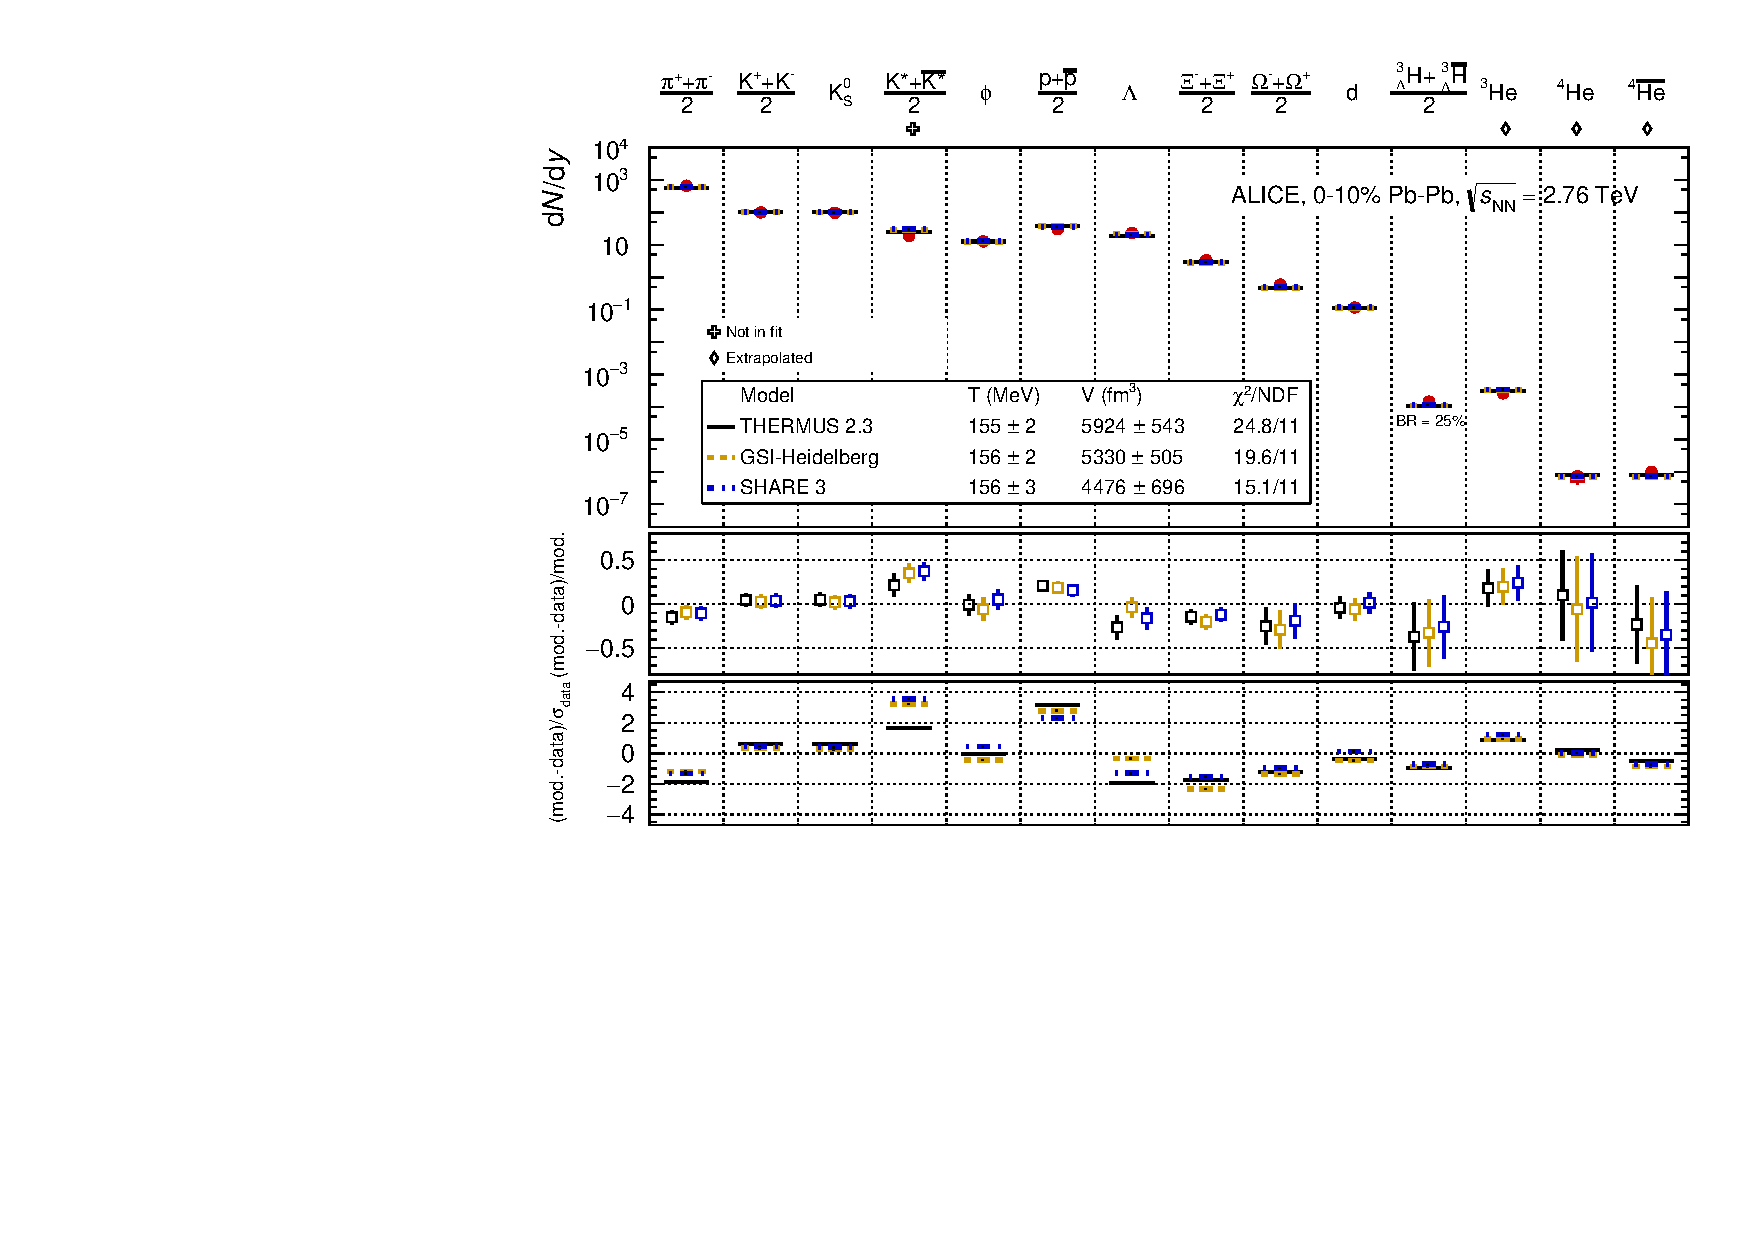
\includegraphics[width=0.75\textwidth]{figures/Fit_PbPb0010_GSITHERMUSSHARE_new_alpha_fixed-91746.pdf}
    \caption{Statistical hadronisation model fits, with three different implementations, to the light flavour hadron yields in central (0-10\%) Pb--Pb collisions at $\sqrt{s_{NN}}$= 2.76 TeV. The data points are taken from  and details of the fits can be found in . The upper panel shows the fit results together with the data, whereas the middle panel shows the difference between model and data normalised to the model value and the lower panel the difference between model and data normalised to the experimental uncertainties. Figure and caption taken from \cite{4He_PbPb}.}
    \label{fig:Stat_Hadron_model}
\end{figure}

The problem with the statistical hadronization model is that it predicts a the production of nuclei from a thermalized medium, when the binding energy of the nuclei is far below the temperature given by the model. For example, the deuteron binding energy is $\approx 2.2$ MeV, compared to the temperature of 156 MeV predicted by the model. This has been dubbed the "snowball forming in hell" problem. Additionally, the statistical hadronisation model says nothing about the underlying mechanism by which the nucleons form antinuclei. \\

The second model is the coalescence model. This model considers the relative momenta of nucleons produced in the collision, and if they are close enough together, assigns them a chance to bond together and form a nucleus. The advantage of this is then that given a set of space and momentum coordinates\footnote{Traditionally coalescence models neglect the spatial correlation part, assuming that the nucleons are close enough together in space to coalesce. And any difference between the sizes of collision systems is then accounted for by a different coalescence parameter.}, the coalescence model can predict the nuclei spectra from the spectra of protons and neutrons. This relation is then experimentally characterized by equation \ref{eq:CoalescenceParameter}:

\begin{equation}\label{eq:CoalescenceParameter}
    B_A = E_A \frac{d^3 N_A}{dp^3_A} \left[ \left( E_{p,n} \frac{d^3 N_{p,n}}{dp^3_{p,n}} \right)^A |_{\vec{p}_p=\vec{p}_n=\vec{p}_A/A } \right]^{-1}
\end{equation}
, where $B_A$ is the coalescence parameter. While this model also requires fits to experimental data in order to give predictions of the yields and spectra of antinuclei, it gives an explanation for the mechanism of how nucleons bond together. For a more comprehensive review of the coalescence model, see \cite{Kachelriess:2020uoh, Coalescence2015}.\\

What can we infer from these models on the production of antinuclei? The important takeaway for this thesis is that their production relies on significant amounts of available energy, and on producing two nucleon close in both space and momentum. These restrictions limit the production of antinuclei to high energy collisions or exotic production channels.

\subsubsection{ Why to we care: antinuclei as a golden channel for new physics}\label{sec:Intro:AntinucleiGoldenChannel}
The main reason why cosmic ray antinuclei make such an interesting probe for new physics is twofold: i) the rarity of the standard model processes which produce them means that any signal does not have to contend with a copious background and ii) that there are already viable theories of new physics -- namely WIMP dark matter -- which predict a detectable antinuclei signal. This has led to the coining of cosmic ray antinuclei as a "smoking gun" for new physics. \\

The first discovery of antimatter in cosmic rays was also the first discovery of antimatter in general: the discovery of the positron in charged particle showers from cosmic rays, in 1932 \cite{positron_discovery}. The discovery of antiprotons in cosmic rays would take almost half a century more, finally being observed in 1979 \cite{antiproton_CR_discovery, Bogomolov:1979hu}. During this time, antiprotons in cosmic rays were a probe into the matter-antimatter asymmetry of the universe, as their abundance could give a hint to the presence of antimatter dominated regions in our galaxy. Their discovery and study to the present day are consistent within uncertainties with production from high energy collisions of cosmic rays with the interstellar medium, providing no evidence for any antimatter dominated regions\footnote{Nowadays constraints on antimatter dominated regions are more stringently set by gamma ray searches.}. The antiproton to proton ratio in cosmic rays is roughly $10^{-4}$. \\

Nowadays, the focus is on the search for antinuclei as a probe of new physics. The expected production from high energy cosmic ray collisions is very low, particularly at low energies (see section \ref{sec:AntinucleiInTheCosmos} for exact values), while several dark matter models predict an antinuclei flux within reach of current or next generation detectors\cite{Doetinchem_2020_review}. The antinuclei of interest are antideuterons and $^3\overline{\mathrm{He}}$. Even though the former is expected to be produced in much greater amount, the same charge and similar mass to the proton make a discrimination harder as for $^3\overline{\mathrm{He}}$, being a charge $Z=-2$ particle. For both, the background in the low energy region (below a few GeV/nucleon) is expected to several orders of magnitude below the expected signal strength. This is in strong contrast to searches involving gamma rays \cite{}, or antiprotons \cite{}, where the signal to background ratio is expected to be on or below the \% level. Thus, an observation of a low energy antinuclei flux would be a sign for new physics. 
%write about the history of the search for antinuclei

\subsubsection{ What affects antinuclei in cosmic rays: production, propagation and annihilation}
As explained in the previous section, low-energy antinuclei in cosmic rays provide a uniquely background free probe into new physics. But in order to interpret any future observation, it is necessary to understand what affects their abundance and spectral shape. These factors can be summed up as 3 things: their production, propagation and annihilation. While a more detailed description of each is given in section \ref{sec:AntinucleiInTheCosmos}, this section aims to give a brief introduction on the importance of the three aspects. \\

The production of antinuclei in cosmic rays can be classed into two categories: i) production in high energy collisions of cosmic rays with the interstellar medium and ii) new, exotic sources. This is different to light nuclei in cosmic rays, whose production is dominated by their production in the stellar cycle. Their production in high energy cosmic ray collisions can be somewhat constrained by experiments at accelerators, which probe fundamentally the same reaction of $p + p \rightarrow \overline{\mathrm{d}}/^3{\overline{\mathrm{He}}} + X$. However, the energies and rapidities at which production mostly occurs are usually at much lower energies than the ones probed by acclerators, e.g. for antideuterons the most important centre-of-mass energy for production in high energy cosmic rays is $\sqrt{s}\approx 25$ GeV (see figure \ref{fig:dbar_2d_source_CR}). Furthermore, the experiments most capable of studying antinuclei, the ALICE experiment at the LHC and the STAR experiment\cite{} at the Relativistic Heavy Ion Collider, probe their production at midrapaidity, rather than at the highly forward rapidities relevant for production in cosmic ray collisions. This means that for much of the relevant parameter space for production, extrapolation from experimental data is necessary. On the other hand, production from new physical processes -- such as the annihilation of WIMP dark matter which is discussed in detail in this thesis -- is even less constrained, and has to be probed by letting Monte Carlo simulations run from an assumed standard model state in the annihilation. \\

Once the antinuclei are produced, they travel through the galaxy until they eventually reach earth. On this journey they are affected by magnetic fields, bulk motion (i.e. diffusion and convection effects), as well as other effects. The good thing is that these affects are the same for all cosmic rays, and can therefore be constrained by observations of more abundant cosmic ray species. Recent work on the topic was done in \cite{Boschini:2017fxq, Boschini:2018baj}, and is explained in more detail in section \ref{sec:AntinucleiInTheCosmos}. \\

On their journey, antinuclei do not merely travel through empty space; the space between stars is filled with the diffuse interstellar medium (ISM), which is made up of about 0.9 protons per cubic centimeter \cite{}. As antinuclei traverse this matter, they might interact and annihilate with it. To account for this loss it is necessary to quantify the inelastic cross section of antinuclei down to low energies. The measurement of these cross sections and the quantification of their effect on antinuclei losses is the topic of this thesis. 
%\subsubsection{ How can antinuclei in the cosmos be detected: AMS, GAPS, cubesats}
%This is all explained towards the end of chapter 5, why rehash it here? 
\subsection{Antinuclei on earth}
On earth, we have the ability to artificially produce antinuclei at high energy physics facilities, like the LHC. In fact, antideuterons were first observed in 1965 in collisions of protons on Beryllium at the Proton Synchrotron\cite{Massam:345976}. Since then, antinuclei have been observed in higher energy collisions in much larger amounts, both at CERN facilities \cite{nuclei_pp_13TeV, nuclei_pp_5TeV, nuclei_pp_PbPb, nuclei_pp}, and heavy ion facilities \cite{}. The ALICE experiment in particular, has published spectra of antinuclei up to $^4\overline{\mathrm{He}}$ \cite{nuclei_pp_13TeV, nuclei_pp_5TeV, nuclei_pp_PbPb, nuclei_pp} in both pp and Pb-Pb collisions. This section aims to give an overview of the studies of antinuclei on earth. 
\subsubsection{Production at accelerators}
Production at accelerators can be classed by energy, and by collisions system. Energy affects the barychemical potential \footnote{The baryochemical potential is a measure of how much more energy is required to produce antibaryons to baryons. A value of 0 means that they are produced in equal amounts, and is found at LHC energies at mid-rapidity\cite{primordial_ratio1, primordial_ratio2}.}, while the collisions system determines the penalty factor for producing heavier (anti)nuclei. The penalty factor -- which describes the amount by which the production of (anti)nuclei is suppressed for each additional nucleon -- is roughly 1/300 in Pb--Pb collisions at 5.02 TeV, while being roughly 1/1000 in pp collisions at 13 TeV \cite{antinuclei_mult_dependence}. The relative $p_T$ integrated yields of nuclei are shown in figure \ref{fig:PenaltyFactorNuclei}. \\

\begin{figure}[h!]
    \centering
    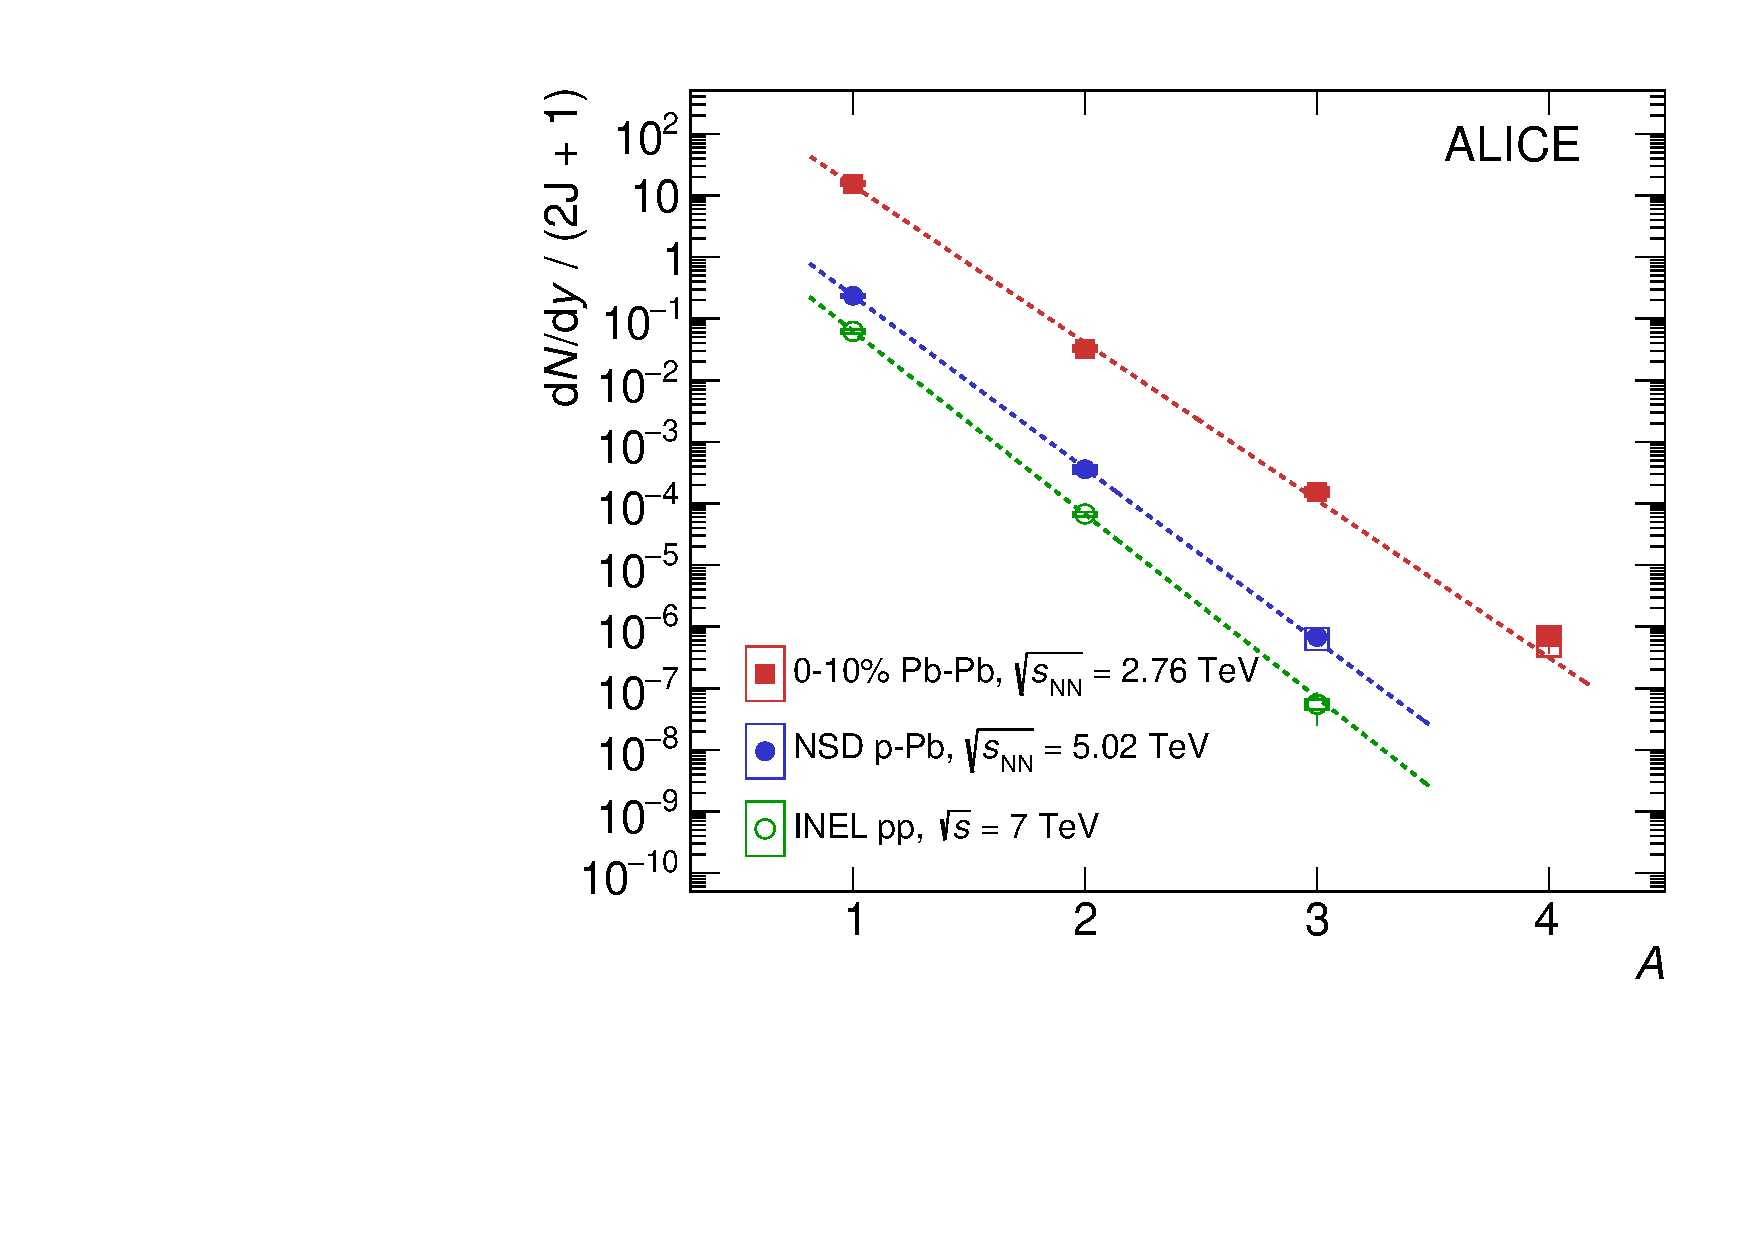
\includegraphics[width=0.8\textwidth]{figures/PenaltyFactor-97548.pdf}
    \caption{Production yield $d\mathrm{N}/dy$  normalised by the spin degeneracy as a function of the mass number for inelastic pp collisions, minimum-bias p-Pb and central Pb-Pb collisions . The empty boxes represent the total systematic uncertainty while the statistical errors are shown by the vertical bars. The lines represent fits with an exponential function. Figure taken from \cite{antinuclei_mult_dependence}.  }
    \label{fig:PenaltyFactorNuclei}
\end{figure}



\subsubsection{Annihilation at accelerators}
Traditionally, annihilations have been studied in fixed target experiments\cite{}. In those experiments, a beam of antiparticles is produced and then fired at a target. The number of particles before and after the target are measured, and the resulting disappearance probability is used to calculate the inelastic cross section. However, this method relies on the ability to produce a clean beam of antiparticles, with sufficient statistics to conduct such an experiment. This comes with two challenges: i) the difficulty of producing antinuclei due to the required energy thresholds and ii) producing the antinuclei in a focused direction, so that they can be captured directed towards a target. These two constraints are unfortunately counterproductive. In order to compensate the difficulty of meeting the energy requirement for the collisions, it is far more energetically favourable to collide in the particles rest frame, however, this produces particles in all directions, not focused towards the beam direction. This makes such measurements increasingly more difficult for higher mass antinuclei.\\

However, since antinuclei up to $A=4$ have been observed in heavy ion collisions \cite{4He_PbPb}, they also have to annihilate in the detector. But it is far more difficult to find an equivalent observable to the fixed target experiment within such an experiment, because it is a priori not possible to know how many particles get produced, and therefore the "loss" of particles is not trivial to measure. The methods developed to measure this loss are the topic of this thesis and will be explained in section \ref{sec:ExperimentAndMethod}, so just a brief introduction is given here. The first method is based on using the knowledge of nuclei production and the baryochemical potential to calculate how many antinuclei should have been produced. The second is based on measuring the particles individually in two different detector systems, and to calculate the loss between the two. 

\subsection{Dark matter and its connection to antinuclei}
In this section a brief introduction into the motivation and evidence for dark matter is given, several prominent dark matter models are discussed, with a particular focus on WIMP dark matter. Furthermore, the connection with WIMP dark matter and antinuclei is discussed. 
\subsubsection{The evidence for dark matter}
The first evidence for dark matter was observed by Zwicky \cite{Zwicky} in 1933, who realised that the rotation curves in galaxy clusters could not be caused solely by the luminous matter observed. His conclusions were not taken seriously until almost 40 years later, when the search for missing mass caused by the advent of cosmology made his theory of dark matter attractive. During this time, the big bang cosmology had prevailed, but left open the question of the ultimate fate of universe. Within big bang cosmology, there are three option. The first is that the universe expands forever, with the gravitational pull merely slowing down the expansion over time, never stopping it. The second is a closed universe, where the density of matter is bigger than some critical density, and therefore will eventually outperform the expansion, causing a collapse of the universe back towards a hot dense medium. And finally, a flat universe, where the density is exactly this critical density, such that eventually the gravitational pull of galaxies will exactly counterbalance the expansion, asymptotically reducing the expansion to 0. From Einstein's theory of general relativity, it can be shown that these fates correspond to the geometry of the universe, and are characterised by a density $\Omega$, where the critical density leading to a flat universe is given by $\Omega_c h^2= 1$\cite{PDG2022, Planck2020}. It was expected that the geometry of the universe is flat\footnote{This means that the local geometry of spacetime is euclidean, which means that all the angles in a triangle in this space add up to 180 degrees. As a counterexample to euclidean space, consider the surface of a sphere, like the surface of earth. It seems locally euclidean, when you lay a triangle on flat ground and add up the angles, they come out to 180 degrees within the measurement uncertainties. But now consider an airplane which starts at the equator flying due north to the north pole. Once it reaches there it makes a 90 degree turn, and flies due south until it once again reaches the equator. It then turns 90 degrees again so it flies along the equator back towards its original destination. The triangle made by the airplane consists of 3 90 degree angles, or 270 degrees. As such, the surface of a sphere like earth is not a euclidean space.}, but observations from galaxy clusters showed that luminous matter only made up a fraction of this density\cite{Planck2020}.%history of dark matter 
Cosmologist turned back to Zwicky's discovery \cite{history_of_dark_matter, Ostriker_return_to_DM}, claiming that dark matter made up the missing mass. \\

More evidence of dark matter was soon to follow. Tracking the rotation curve in galaxies provided evidence for dark matter bound in galaxies\cite{Sofue2020, Sofue_2016, history_of_dark_matter}. Measuring the dispersion velocities of galaxies around either other galaxies (such as the velocities of dwarf galaxies around a more massive one) or around galaxy clusters provided evidence for dark matter trapped in larger gravitationally bound structures, as did gravitational lensing\cite{Cluster_lenses}. For a comprehensive review of the evidence for dark matter see the particle data group \cite{PDG2022}. Each piece of evidence points to a type of matter which does not interact electromagnetically (hence "dark"), and makes up the majority of the mass found in cosmic structures. \\

Further evidence for dark matter can be found in structure formation in cosmology. From anisotropies in the cosmic microwave background (CMB), it can be inferred that at the time of CMB decoupling the baryonic density fluctuations were of order $\delta\rho_\mathrm{rec} / \rho \approxeq 10^{-5}$. Since these fluctuations scale linearly with the expansion of the universe, today's baryonic density anisotropies can be calculated as $\delta\rho_b / \rho |_\mathrm{today}\approxeq 10^{-2}$\cite{PDG2022}. Since matter is highly concentrated into galaxies in the present day universe, fluctuations are $\delta\rho_b / \rho |_\mathrm{obs}>> 1$. This discrepancy can be solved by adding a dominant non-relativistic, collisionless component the mix, which decoupled from thermal equilibrium well before the CMB. In other words, in order to explain structure formation from the early universe, one needs a dominant component of the mass to be in a form which does not interact electromagnetically, and does not heavily self-interact, which is also what is needed in order to explain the present-day observations of galactic motion. \\

Finally, it is important to discuss the difference between hot and cold dark matter. Dark matter which was thermally produced in the early universe -- called a thermal relic -- can be split into two categories: hot relics, which were still ultra-relativistic when they decoupled from thermal equilibrium, and cold relics, which were no longer relativistic, or cold enough to significantly cool from the expansion of the universe. Due to the different velocities of these relics, hot relics are expected to cause sharp features in the large scale structure of the universe, while cold dark matter is expected to cause a smooth large scale structure. This can be understood as how easily a particle is trapped in a gravitationally collapsed structure. After an initial overdense region forms and a gravitational well builds, slow (cold) particles will be trapped in the well first, while fast (hot) particles will not be trapped in the well until the gravitational well becomes much deeper. To get an idea of the order of magnitude of velocities, consider the escape velocity of our galaxy, which lies around 600 km/s \cite{MW_escapeVel}, which is equivalent to $\beta \approxeq 2 \times 10^{-3}$. Thus, relativistic particles would provide a counterbalance to the formation of gravitationally collapsed structures, and thus require deeper wells for large scale structures to form. This feature can be seen in \ref{fig:LargeScaleStructure}, which shows that the large scale structure of our universe prefers the cold dark matter model. 

\begin{figure}[h!]
    \centering
    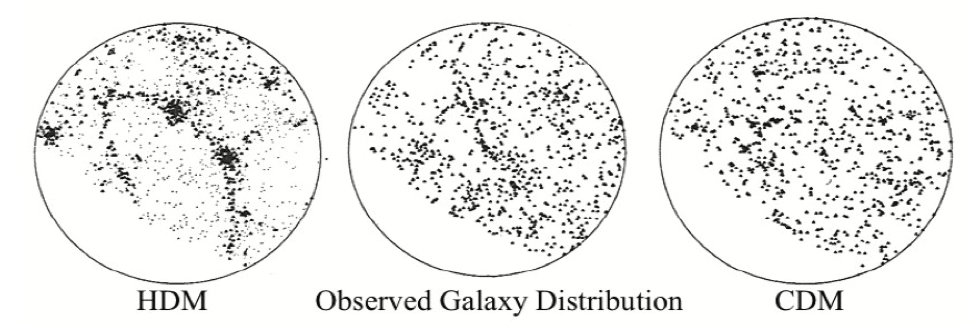
\includegraphics[width=\textwidth]{figures/Galaxy_distributions_by_DM_type.png}
    \caption{Computer simulations of the distribution of galaxies within our universe, with hot dark matter (left) and cold dark matter (right), compared to the observed distribution (middle). Figure is taken from \cite{Ibarra_neutrinos}. }
    \label{fig:LargeScaleStructure}
\end{figure}


\subsubsection{WIMP dark matter and the WIMP miracle}\label{sec:IntroWIMPs}
WIMP dark matter is candidate model for dark matter, which explains dark matter as heavy particles which only interact gravitationally an through the weak force. WIMPs are a tempting choice for dark matter, since their properties could explain all the observed phenomena (galactic motion and structure formation). A WIMP is a stable particle\footnote{The WIMP lifetime must be greater than the current age of the universe, since otherwise most would have decayed by now.}, with a mass from a few GeV to a few TeV. At their inception there were several promising WIMP candidates from supersymmetric expansions to the standard model, although since then the parameter space available for WIMPs has been probed and become far more constrained. But the real allure of the WIMP is the WIMP "miracle". \\

The WIMP miracle is well known to be the fact that when one considers a particle of the weak mass scale with a self annihilation cross section close to the weak interaction strength (on the pb level), the present day dark matter relic density can be obtained. Additionally, in many versions of supersymmetry, the lightest supersymmetric particle is indeed a weakly interacting heavy particle, the ideal scenario for the WIMP\cite{Supersymmetry_primer}. In the following section the derivation of the WIMP abundance is shown, which is reproduced here from \cite{BAER20151}. The WIMP is denoted as $\chi$, and it is assumed be in thermal equilibrium with other matter while the Temperature is $T>$\dmm . During this time, the WIMP density $n_\chi$ evolves according to the Boltzmann equation, shown in equation \ref{eq:boltzman_deriv_eq}: 
\begin{equation}\label{eq:boltzman_deriv_eq}
    \frac{dn_\chi}{dt} = -3H n_\chi - <\sigma_{ann}v>(n_\chi^2 - n_{eq}^2)
\end{equation}
where $H$ is the Hubble constant at that time, which in a radiation dominated universe\footnote{The universe was dominated by radiation until roughly 47ky after the Big Bang, which is many orders of magnitude longer than the dark matter decoupling time, which is at $\lesssim$ 1 s.} is given by $H^2 = \rho_{rad}/3M^2_P$, where $M_P$ is the plank mass. While the system is in equilibrium, the number density tracks the equilibrium density $n_{eq}$. Subsequently, at some temperature $T_f$<m$_\chi$, the expansion rate will exceed the annihilation rate, and dark matter will freeze out, and their comoving number density (i.e. the number density accounting for the volumetric expansion of the universe) will remain constant from this point on. An approximate solution to the Boltzmann equation at this point gives equation \ref{eq:sol_Boltzmann}, where $\Omega_\chi h^2$ is the dimensionless dark matter density in the universe\footnote{$\Omega_\chi$ can be interpreted as the curvature of space which dark matter is responsible for.}, $s_0$ is the present day entropy density of the Universe, $g_*$ is the number of relativistic degrees of freedom of the particle $\chi$ at freeze out, and $x_f = T_f/m_\chi \approxeq 1/25$ is the freeze out temperature scaled to the dark matter mass. The value for $x_f=1/25$ is obtained from solving the Friedmann equation\footnote{This is the solution to Einstein's field equations for an open, closed or flat universe.} numerically for the freezeout Temperature (see \cite{BAER20151} for more details). This means that WIMPs would have still moved at relativistic speeds at freezeout, with velocities $<v>\approx c/3$. 

\begin{equation}
    \label{eq:sol_Boltzmann}
    \Omega_\chi h^2 \approx \frac{s_0}{\rho_c/h^2} \left( \frac{45}{\pi^2g_*}\right)^2 \frac{1}{x_f M_P} \frac{1}{<\sigma_{ann}v>}
\end{equation}

Plugging in the known values for the parameters\cite{ref 533 DM review} and setting $\Omega_\chi h^2$ = 0.12 from the latest Planck Collaboration results \cite{Planck2020}, one obtains equation \ref{eq:DM_relic_density}. 

\begin{equation}
    \label{eq:DM_relic_density}
    \frac{\Omega_\chi h^2}{0.12} = \frac{1}{\frac{<\sigma_{ann}>}{10^{-36} cm^2} \frac{v/c}{0.1}}
\end{equation}

Thus, setting the thermally averaged annihilation cross section to a value of 1pb * $c$, and using average velocities of the order one would expect from a WIMP at freezeout, the current dark matter abundance is recovered. A schematic representation of this process is shown in figure \ref{fig:DM_thremal_eq_freeze_out}, where the decoupling temperature $T_{dec}$ and the freezeout temperature $T_{f}$ are shown separately. The decoupling temperature is the temperature at which the dark matter and luminous matter stop being in thermal equilibrium, while the freeze out temperature the point where the expansion rate becomes the dominant term for the density change for dark matter, over the annihilation term. 

\begin{figure}[h!]
    \centering
    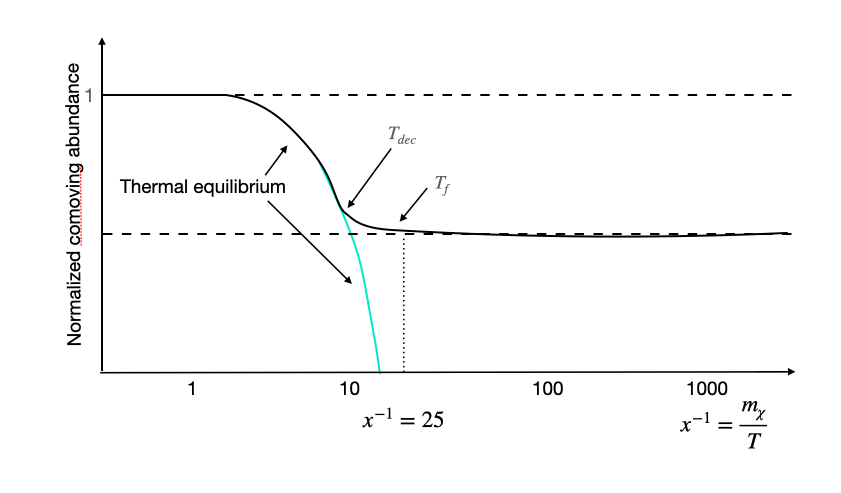
\includegraphics[width=\textwidth]{figures/schematic_thermal_eq_evolution_DM.png}
    \caption{Transition of dark matter from thermal equilibrium to freeze out. Both the decoupling temperature (where dark matter stops being in thermal equilibrium with luminous matter) and the freeze out temperature (when the rate of expansion has dropped the annihilation rate to negligible amounts, so that the comoving density can be considered constant) are indicated on the schematic. Figure is based on the figure in \cite{Baer}}
    \label{fig:DM_thremal_eq_freeze_out}
\end{figure}



\subsubsection{Other dark matter models}\label{IntroOtherDM}
WIMP dark matter is not the only dark matter model on the market, indeed, dark matter models span over $\approx$ 30 orders of magnitude in mass. A collection of models and their mass ranges is shown in figure \ref{fig:DarkMatterModelsSummary}. Notable other dark matter candidates are neutrinos, sterile neutrinos, axions and primordial black holes (not shown in figure \ref{fig:DarkMatterModelsSummary}). In this section we shall briefly discuss their main concepts, advantages and disadvantages. Promising candidates usually share the quality that they solve not just the nature of dark matter, but also another problem in physics. As discussed earlier, the WIMP neutralino was considered the supersymmetric extension to the standard model at its inception.\\

\begin{figure}[h!]
    \centering
    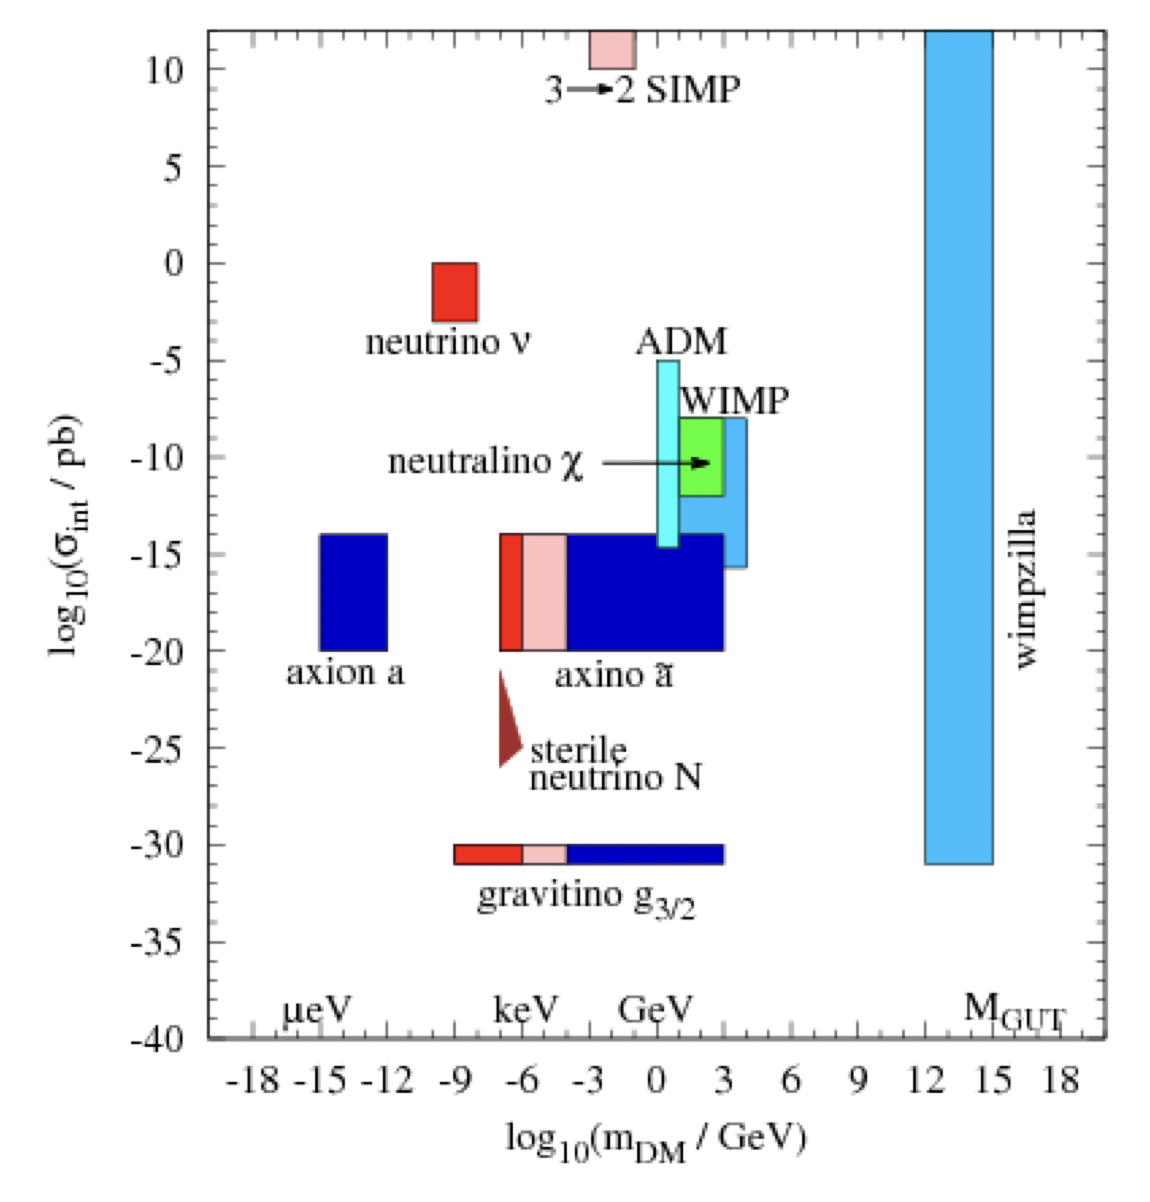
\includegraphics[width=\textwidth]{figures/DM_summary_models.png}
    \caption{Collection of candidate dark matter models over a wide mass range. The most prominent candidates are WIMP dark matter, axion dark matter and sterile neutrinos. Primordial black hole dark matter is not shown on this plot. Figure taken from \cite{BAER20151}.}
    \label{fig:DarkMatterModelsSummary}
\end{figure}



Let us first consider axion dark matter. Axions arise naturally in the Peccei-Quinn (PQ) solution to the strong CP problem\cite{PQ_axion, Weinberg} (see section \ref{sec:IntroSymmetries} for more details), by arguing that the CP violating term $\bar{\theta}$ of the QCD Lagrangian is relaxed to 0 due to an additional PQ symmetry. This symmetry is accompanied by a scalar field which spontaneously breaks the symmetry at low energy, giving rise to the axion. While the initial model, which predicted axion masses of order O(100keV) has long since been experimentally ruled out, it has been replaced by models using the same mechanism to dynamically solve the strong CP problem. Axions of such fields are expected to have masses in the $\mu$eV range. As a side effect, the scalar field would populate the universe with axions, which -- since they are produced non-thermally at rest\cite{cookbook} -- would be considered cold dark matter even though they have such low masses. As such, a dark matter theory which is not at least partially made up of axions has to provide an alternate solution to the strong CP problem. \\

Out of all the standard model particles, the neutrino is the only particle which does not interact through either the strong or electromagnetic forces. This makes it a promising initial candidate for dark matter. However, the present-day abundance of neutrinos would be given by equation \ref{eq:NeutrinoAbundance} (further details can be found in \cite{BAER20151}). Current constraints on the sum of the neutrino masses $\sum m_\nu$ limit the amount of dark matter in the form of neutrinos to about 0.5\%-1.6\% \cite{PDG2022}. These constraints come from neutrino mixing experiments, as well as from cosmological bounds. This is because neutrinos -- being hot dark matter -- have a direct impact on large scale structure formation. A related dark matter model is that of sterile neutrinos. This group of models postulates that the right handed neutrinos (and left-handed antineutrinos), are far more massive than their chiral partners. Since they interact only gravitationally (neutrinos carry no electromagnetic or color charge, and the weak force couples only to left-handed neutrinos and right-handed antineutrinos), they would constitute a viable candidate for dark matter\cite{}. Recent observations of neutrino mixing \cite{}, show that neutrinos are not massless but have a finite mass. The higgs mechanism responsible for giving SM particles their mass requires both left-handed and right-handed fermions \cite{}, and thus suggests the existence of the neutrinos' chiral partners. Their mass also means that their chirality is not relativistically invariant, since their velocities are slower than the speed of light; i.e. it is possible for an observer to travel faster than the neutrinos and thus observe them with a different chirality. However, it is not known why the couplings to for the left- and right-handed neutrinos would be so different. \\

\begin{equation}\label{eq:NeutrinoAbundance}
    \Omega_\nu h^2 = \frac{\sum m_\nu}{91.5 \mathrm{eV}}
\end{equation}

The final dark matter candidates to consider are primordial black holes. They are discussed more closely in section \ref{Res:PBH}, but a brief overview is given here for completeness. Very shortly after the big bang (O($10^{-23}$)s), overdense regions in the universe might have collapsed into black holes. Depending on the time of their formation, they would have consumed most the of available mass within their observable universe at the time, i.e. within their horizon. Such black holes would have expected masses today ranging over many orders of magnitude, well below the critical mass for a stable black hole \cite{HAWKING1974}. Black holes below this mass tend to radiate energy off at a rate faster than their mass accretion, via Hawking radiation \cite{VISSER_2003, HAWKING1974}. The rate at which such small black holes radiate off energy is higher the smaller they are, meaning towards the end of their lifetime they disappear via runaway evaporation. During such a process, new antiparticles and particles can be produced. Such primordial black holes fit the required properties of dark matter, being colissionless uncharged matter which interacts gravitationally. However, due to null observation of the particles expected to be released from the evaporation of black holes, their abundance can be tightly constrained. As such, they can at most make up a tiny fraction ($\approx 10^{-11}$) of the observed dark matter in our galaxy.

\subsubsection{Dark matter annihilations into antinuclei}
The null results from searches for direct detection of WIMPs, either from evidence for supersymmetry at the LHC or from direct detection experiments \cite{XENON2, Lux}, have motivated other probes for WIMPs. Antinuclei observations from WIMP annihilations have become one of the most promising of such probes, since many WIMP candidates are expected to produce a detectable flux of low energy antinuclei\cite{Ibarra:2012cc, Korsmeier:2017xzj}. By definition WIMPs can couple weakly to standard model particles, and their wide plausible mass range leaves open a large parameter space with sufficient energy to create antinuclei. Additionally, since dark matter is expected to be cold, the production of antinuclei occurs in the galactic rest frame, providing no boost to artificially increase their momentum. Thus, considering WIMP annihilations into an initial standard model state, the production of antinuclei is plausible. In a given point in space, the amount of antinuclei produced is then dependent on the number of dark matter annihilations times the spectrum of produced antinuclei in such annihilations, as given in equation \ref{eq:IntroDM_source_term}

\begin{equation}\label{eq:IntroDM_source_term}
    q(\vec{r}, E) = \frac{1}{2} \left( \frac{\rho_{\chi}(\vec{r})}{m_\chi}\right)^2 <\sigma v > (1+\epsilon) \frac{dN}{dE}
\end{equation}
, where $\rho_\chi$ is the measured dark matter density at a given point, and (1+$\epsilon$) accounts for the contribution from other annihilation products which later decay into the antinucleus in question. This process is discussed in more detail in section \ref{sec:AntinucleiInTheCosmos}.


\subsubsection{Majorana vs. Dirac dark matter}\label{sec:IntroMajoranaDiracDM}
To current knowledge, every fermion in the standard model has an antiparticle, with the same mass and quantum numbers, but opposite charge. This was first predicted by Paul Dirac, who realised that the wave equation he developed to account for special relativity in the motion of electrons implied a second solution, corresponding to a particle with opposite charge\cite{Dirac}. This particle, the positron, was subsequently discovered, and was the first discovery of antimatter\cite{positron_discovery}. \\

However, it is mathematically possible for a particle to be its own antiparticle; such particles are called Majorana particles. Out of the fermions in the standard model, only the neutrino could be a majorana particle, since all other fermions have known antiparticles. The majorana nature of the neutrino is being investigated by searching for neutrinoless double beta decay, a process by which two beta decays happen almost simultaneously, the produced neutrinos annihilate and thus provide additional energy to the electrons. The GERDA experiment is currently looking for such an effect \cite{GERDA}, but has so far found no signal. \\

WIMP dark matter is often assumed to be a majorana fermion. Given the lack of any known majorana particles, this seems somewhat unintuitive. The reason is mainly historical, since the original motivation for the WIMP was the supersymmetric neutralino, which is a hypothetical Majorana particle \cite{Supersymmetry_primer}. The reason this convention is still used, is that the effects of the assumption on the Dirac or Majorana nature of a WIMP are degenerate with the assumed WIMP self-annihilation cross section and therefore they produce the same signal. To show this, let us consider equation \ref{eq:IntroDM_source_term}, which describes the source term for antinuclei from Majorana dark matter annihilations. The Dirac nature of the WIMP enters the equation in two ways. First, the density considered. Since the total gravitational effect of dark matter is known, the total measured dark matter density is the sum of the densities of dark matter and anti dark matter $\rho_{\mathrm{DM}}^{\mathrm{meas}} = \rho_\chi  + \rho_{\overline{\chi}}$.Thus -- assuming symmetric populations of dark matter and anti-dark matter -- the density term in equation would be $\rho_\chi \rho_{\overline{\chi}} = \frac{\rho_{\mathrm{DM}}^2}{4}$. This is a factor of 2 lower than original density term (the symmetry factor of 1/2 in equation \ref{eq:IntroDM_source_term} is due to the Majorana nature and thus falls away). However,the second effect is on the thermally averaged annihilation cross section $<\sigma v>$. When predicting the value of $<\sigma v>$ required for the currently observed abundance (as was done in section \ref{sec:IntroWIMPs}) the same density alteration is required, which means that the prediction for the thermally averaged cross section remain the same. This is shown in figure \ref{fig:sigmaV_DiracvsMajorana}. Thus, these two effects cancel, yielding the same results for Dirac or Majorana dark matter. \\

\begin{figure}[h!]
    \centering
    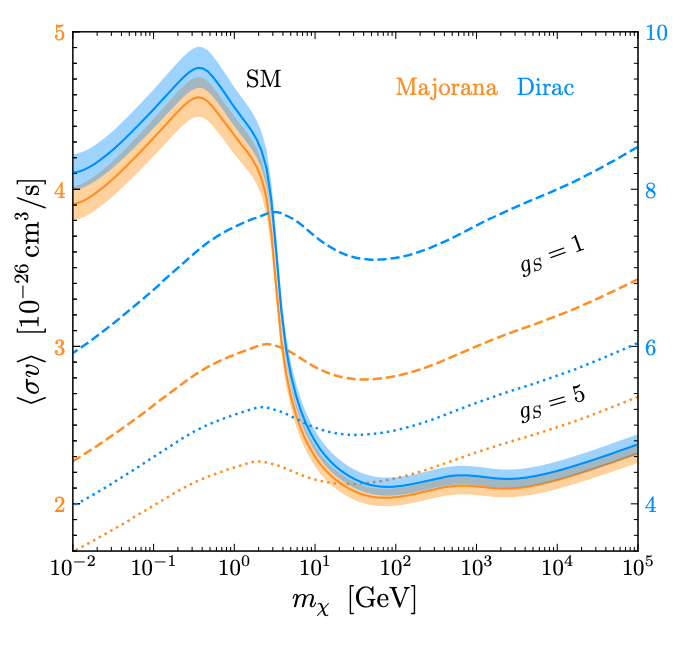
\includegraphics[width=0.7\textwidth]{figures/sigma_v_dirac_majorana_dm.png}
    \caption{Thermally averaged annihilation cross section for WIMP dark matter necessary to reproduce the measured present-day abundance of dark matter. The left y-axis shows the values for Dirac dark matter, while the right y-axis shows the values for Majorana dark matter, showing the difference of a factor 2. Taken from \cite{}. }
    \label{fig:sigmaV_DiracvsMajorana}
\end{figure}

The only possible difference between the two models would come from an asymmetry in the population of dark matter and anti dark matter, and only if this was created after decoupling. If the asymmetry was caused prior to decoupling, the derivation for the expected WIMP cross section would account for this. Thus, such an asymmetry would have had to be caused by a process after dark matter decoupled from thermal equilibrium, which suggests it would have had to form through purely dark matter interactions. It is therefore difficult to suggest any process which would cause such an asymmetry. However, assuming an asymmetry was formed, the number of annihilation would be reduced by the factor $4x(1-x)$ in respect to the case of symmetric Dirac dark matter, where $x = \rho_\chi / \rho_{\chi + \overline{\chi}}$ is the asymmetry factor. For further discussion of asymmetric dark matter, see section 4D in \cite{BAER20151}. 

%\subsubsection{The distribution of dark matter within our galaxy}
%This is carefully explained in a later section, doesnt need to be explained here i think. 
\subsubsection{The search for dark matter: the link between WIMP dark matter and antinuclei}
Searches for dark matter can be classed into 3 categories: production searches, direct detection experiments and astrophysical searches. Production searches look to detect the production of dark matter particles in high energy collisions at accelerators. Technically, if WIMP dark matter is weakly interacting and within a mass range which can be produced at accelerators, it might be detectable. However, there is currently no evidence for the production of dark matter at accelerators. Such production searches usually form only a small part of the physics programs of accelerator experiments. The second category of experiments are direct detection experiments. These experiments look for WIMP-nucleon interactions and the corresponding recoil, and include the XENON \cite{XENON_new_physics, XENON2} and LUX collaborations\cite{Lux}. These will be discussed in more detail in section \ref{sec:AntinucleiInTheCosmos}.\\

The final probes are astrophysical searches. These focus on signals produced by potential WIMP dark matter which can be differentiated from standard model sources. These signals can come either from annihilations or decay of WIMP dark matter\footnote{Technically WIMP dark matter could also scatter of baryonic matter, but this would be much easier to observe in direct detection experiments than in space.}, and we have to chose detection channels in which we could both get a reliable signal and differentiate it from other cosmic sources. The most promising searches are gamma rays and antinuclei \cite{Conrad2017}, both of which could be produced in the annihilation of many WIMP candidates, and would produce signals which are expected to be distinguishable from common astrophysical backgrounds. This thesis focuses on measuring antinuclei inelastic cross section and their effect on such an antinuclei signal, in order to help interpret any future antinuclei measurements in cosmic rays.


%\subsection{Dark matter and its connection to antinuclei}

\subsubsection{The evidence for dark matter}
\subsubsection{WIMP dark matter and the WIMP miracle}\label{sec:IntroWIMPs}
\subsubsection{Dark matter annihilations into antinuclei}
\subsubsection{Majorana vs. Dirac dark matter}\label{sec:IntroMajoranaDiracDM}
Since the properties of dark matter are not know beyond its gravitational pull, it is also not known if dark matter is its own anti-particle. 
\subsubsection{Thermal self-annihilation cross section in the early universe}
\subsubsection{The ditribution of dark matter within our galaxy}
\subsubsection{The search for dark matter: the link between WIMP dark matter and antinuclei}
\newpage
\section{Experimental data and experimental method}

\subsection{ALICE}
\subsubsection{Overview}
\begin{itemize}
    \item Trigger System
    \item ITS
    \item TPC
    \item TOF
\end{itemize}

\subsubsection{Basics of ALICE data structure}
\subsubsection{Collision system and event cuts}
\subsubsection{Reconstruction of raw (anti)nuclei}
\subsubsection{Raw \ratio\ \ ratio}
\subsubsection{Raw antitriton-to-triton ratio}
\subsubsection{Correction for secondaries from material spallation}
\subsubsection{Annihilations within the detector}


\subsection{Extracting the inelastic cross section from the antimatter-to-matter ratio}
The idea behind using the antimatter-to-matter ratio as the observable to measure the antinuclei inelastic cross section, is that antinuclei will annihilate in the detector material, and therefore disappear from our measurement. In order to quantify the inelastic cross section we thus need to know how many particles were originally produced, i.e. we need to normalise the antinuclei spectrum to the number of originally produced antinuclei. However, we cannot use theoretical predictions tuned to this data, since that would be a circular argument, i.e. we would get out the same inelastic cross section as we put in. Therefore, the matter nuclei are used as a proxy instead. This works very well for a few reasons. First, the matter inelastic cross section can be easily measured, and have been measured for deuterons \cite{}, helium-3\cite{} and tritons\cite{}. Second, other effects affecting acceptance or efficiency will largely cancel between the nuclei and antinuclei counterparts, since the two only differ in their charge sign. Third and perhaps most important, is the fact that at LHC energies, the baryochemical potential is very close to 0, and has been accurately measured for antiprotons. This means that we know to a very high degree of accuracy how many antinuclei are produced relative to the produced nuclei, and the other processes by which both might be lost within the detector are also well understood. Thus, the antimatter-to-matter ratio is sensitive to the antinuclei inelastic cross section, and other variables it is sensitive to are well understood and under control. This makes this ratio such a promising probe to measure the inelastic cross section.\\

Having established that the antimatter-to-matter ratio is sensitive to the inelastic cross section, it is still not trivial to extract the inelastic cross section from this observable. This difficulty is due to having to account for many processes. One example is the path which the particles take through the detector. In the magnetic field, (anti)nuclei travel on curved tracks, so the amount of matter they interact with will depend on their initial trajectory. This thus needs to be averaged over the $\eta$ distribution of the antinuclei. This is just one of many similar effects which make an analytical relationship between the antimatter-to-matter ratio and the antinuclei inelastic cross section difficult to achieve. Thankfully, there is a superior option with detailed Monte Carlo simulations. Detailed simulations of the ALICE detector using Geant4 account for such processes, and by changing the inelastic cross section in these simulations, we can probe its relationship to the antinuclei-to-nuclei ratio.
\subsubsection{Comparison of ratios with Monte Carlo simulations}\label{sec:MCSim}
In order to fairly compare the Monte Carlo simulations to the produced data, it is vital to account for the baryochemical potential\footnote{In other words: how much more antimatter particles we have for each matter particle. Given that we collide purely matter particles, there is a penalty for producing antimatter, even though at such high energies it is vanishingly small.} at such high energies. The relevant ratio of antiprotons to protons is shown in figure \ref{fig:BaryochemicalPotential}. Based on the same arguments as the formula for the coalescence parameter \ref{eq:CoalescenceParameter}, the effect on the ratio of antinuclei will be the same as to the antiproton-to-proton ratio taken to the exponent of the mass number of the antinucleus. 

\begin{figure}
    \centering
    \includegraphics{}
    \caption{Ratio of antiprotons to protons produced at mid-rapidity as a function of beam rapidity. At ALICE energies the value approaches unity, demonstrating that at such high energies antimatter and matter are produced in almost equal amounts.}
    \label{fig:BaryochemicalPotential}
\end{figure}
\subsubsection{Ratios as a function of the inelastic cross section}
\subsubsection{Non-linear error propagation}
\subsubsection{Accounting for energy losses between the primary vertex and the point of annihilation}
\subsubsection{Uncertainty coming from the material budget}
\subsubsection{Evaluating the average material for antinuclei annihilations in the ALICE detector}
\subsubsection{Independence of collision system}
The antimatter-to-matter ratio method's dependence on collision system has been investigated by redoing the analysis performed in pPb collisions in \cite{dbarIvan} for high multiplicity pp collisions. The dependence on the collision system is due to the multiplicity differences, and the resulting difference in the baryochemical potential as discussed in section \ref{sec:MCSim}. By taking the antiproton-to-proton ratio for the different collision systems and comparing them, the predicted difference between the antideuteron-to-deuteron ratio was obtained. The results are shown in figure \ref{fig:pp_pPb_dbardRatio}, which show that the differences between collisions systems are consistent with the expected deviation. This independence of the collision system is expected, since the inelastic cross section is completely independent on the collision system. This becomes especially self-evident when considering that the annihilations do not occur in the initial collisions, but rather as the antiparticles travel through the detector material.

\begin{figure}[h]
    \centering
    \includegraphics{}
    \includegraphics{}
    \caption{Ratio of the antiproton-to-proton ratios (left) and antideuteron-to-deuteron ratios (right) obtained in high multiplicity pp collisions and in pPb collisions, compared to the expected difference from the different baryochemical potentials (dashed red line).}
    \label{fig:pp_pPb_dbardRatio}
\end{figure}


\newpage








\section{Measurement of the \ahe\ inelastic cross section}\label{sec:ResHe3SigmaInel}
The measurement of the \ahe\ inelastic cross section is the most fundamental result of this thesis. This is the first measurement of this inelastic cross section, which is important not just for nuclear physics, but also for astrophysical searches for physics beyond the standard model, as discussed in section \ref{sec:Intro:AntinucleiGoldenChannel}. Historically, inelastic cross section measurements were done using fixed target experiments: a beam of the particle of interest was isolated, and then fired on a material target. By measuring the abundance of the particle before and after the target, the cross section could be measured. The difficulty in doing this for antinuclei lies in the production and isolation of an antinuclei beam, since antinuclei production is so rare and has a high $\sqrt{s}$ threshold. Even at the places where antinuclei are produced (at the LHC and at high energy heavy-ion facilities\cite{}), further isolating a beam of such particles is not feasible. In fact, out of all antinuclei ($A$>2), this method has only been applied to high energy antideuterons \cite{}, at the CERN proton synchrotron in the 70s, for particles at very high momenta of 13 GeV/$c$ and 25 GeV/$c$. Recently, roughly half a century later, the new measurement technique using the antiparticle-to-particle ratio has been shown to be able to measure the antideuteron inelastic cross section down to 500 MeV/$c$ \cite{antideuteronXS}. This measurement has now been expanded to \ahe\ \cite{antiHe3XS} and \atrit\ , and a separate complementary method (TPC/TOF method) has enabled the use of the high statistics Pb--Pb data to boost the measurements' precision. Both these new methods rely on quantifying the absorption of antinuclei as they travel through the detector material, rather than a dedicated target. The disadvantage of this approach is that the detector material is optimised to have little material budget as possible, as to not interfere with the particles of interest. Nevertheless, these methods allow us to further our knowledge of antinuclei inelastic cross sections for the first time in half a century.
\subsection{Physics motivation and overview of the analysis method}
\subsection{Analysis techniques}
\subsubsection{Antimatter-to-matter ratio method}

\subsubsection{TOF-TPC matching method}
The second method for measuring \sigmainel\ uses the fact that \ahe\ can be clearly identified in the TPC, and then those tracks can be checked again in the TOF. This method works akin to a fixed target experiment, in that a "beam" is identified by measuring \ahe\ in the TPC, this beam is then fired upon the "target", which in this case is the space frame and the TRD. Some of the nuclei will annihilate, while the others who make it through will generate a matching TOF hit, thus enabling a measurement of how much of the beam survives. \\
The advantage of this method is that only the antiparticles are required; no specific assumptions about the antimatter-to-matter ratio need to be assumed and tested. This also means that secondary correction need not be applied, since the origin of the \ahe\ has no impact on the result\footnote{Also, there are no secondary \ahe\ nuclei from material spallation, so the secondary correction is even less important.}. The disadvantage is that the acceptance of the TOF detector limits the applicability of this method to higher momenta, so it is more difficult to measure the low energy rise of the inelastic cross section. \\

The measurement of \sigmainel\ using the TPC-TOF matching method is thus complementary to the antiparticle-to-particle method described above. This analysis was not carried out as part of this work, but ties in closely with the results shown both in this chapter and in chapter \ref{sec:AntinucleiInTheCosmos}, and is thus described here. The measurement is also shown together with the measurement using the antimatter-to-matter inelastic cross section. More details about the analysis can be found in \cite{PavelAN, antiHe3XS}.

\subsection{Secondary correction}
\subsection{Results}


\newpage
\section{Measurement of the antitriton inelastic cross section}\label{sec:ResTritonSigmaInel}
\subsection{Physics motivation and overview of the analysis method}
The measurement of \sigmainelH\ does not have the same astrophysical motivation as the measurement of \sigmainel\ , since \atrit\ is an unstable nucleus with a half-life of $\approx 12.3$ years. Instead, the main motivation for this measurement is the comparison to the \ahe\ inelastic cross section. This could shine light on any isospin dependence of the annihilation probability of antinuclei. Such an effect might also elucidate how the strong force interacts with isospin, in a potentially more sensitive way than observing neutrons, since they are much harder to detect due to not being charged. And while the current statistical uncertainties are unable to resolve any difference, the two measurements provide a proof of concept that this dependence can be measured by means of comparing the inelastic cross sections of $A=3$ antinuclei.
\subsection{Accessible momentum range of the measurement}
\begin{figure}
    \centering
    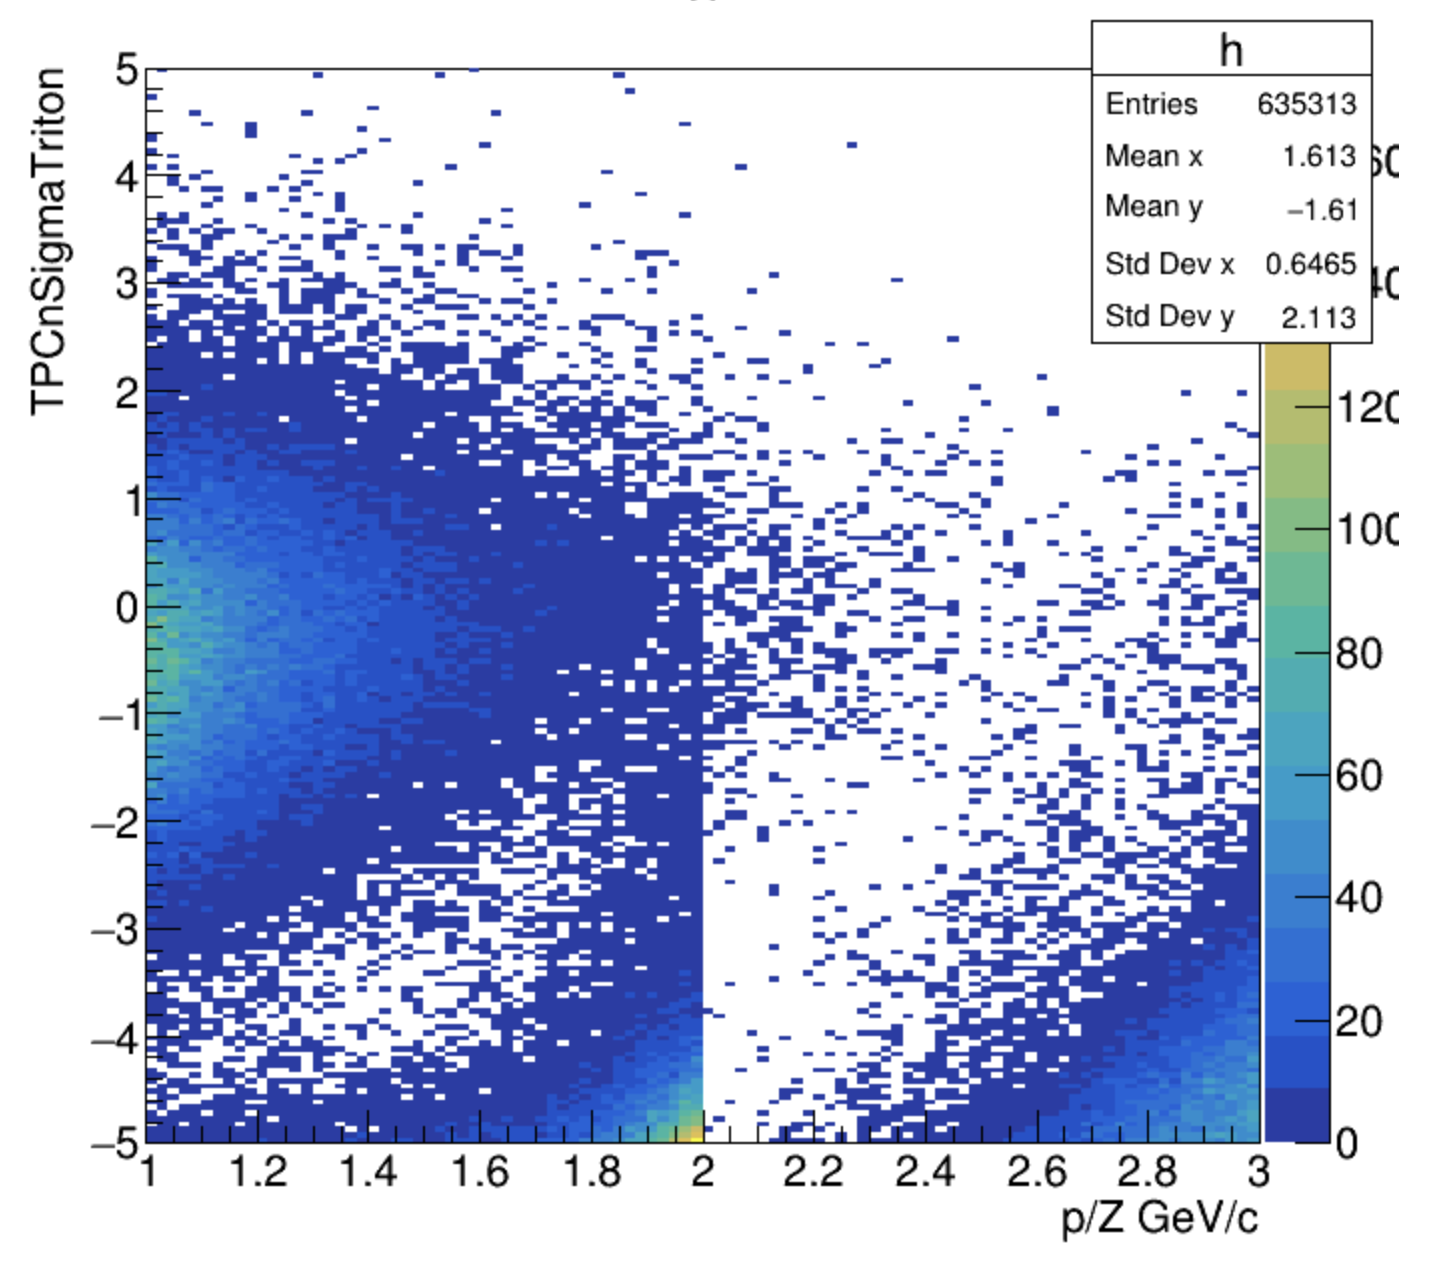
\includegraphics[width=0.48\textwidth]{figures/triton/tbar_TPCnSigma_noTOF_noDCA.png}
    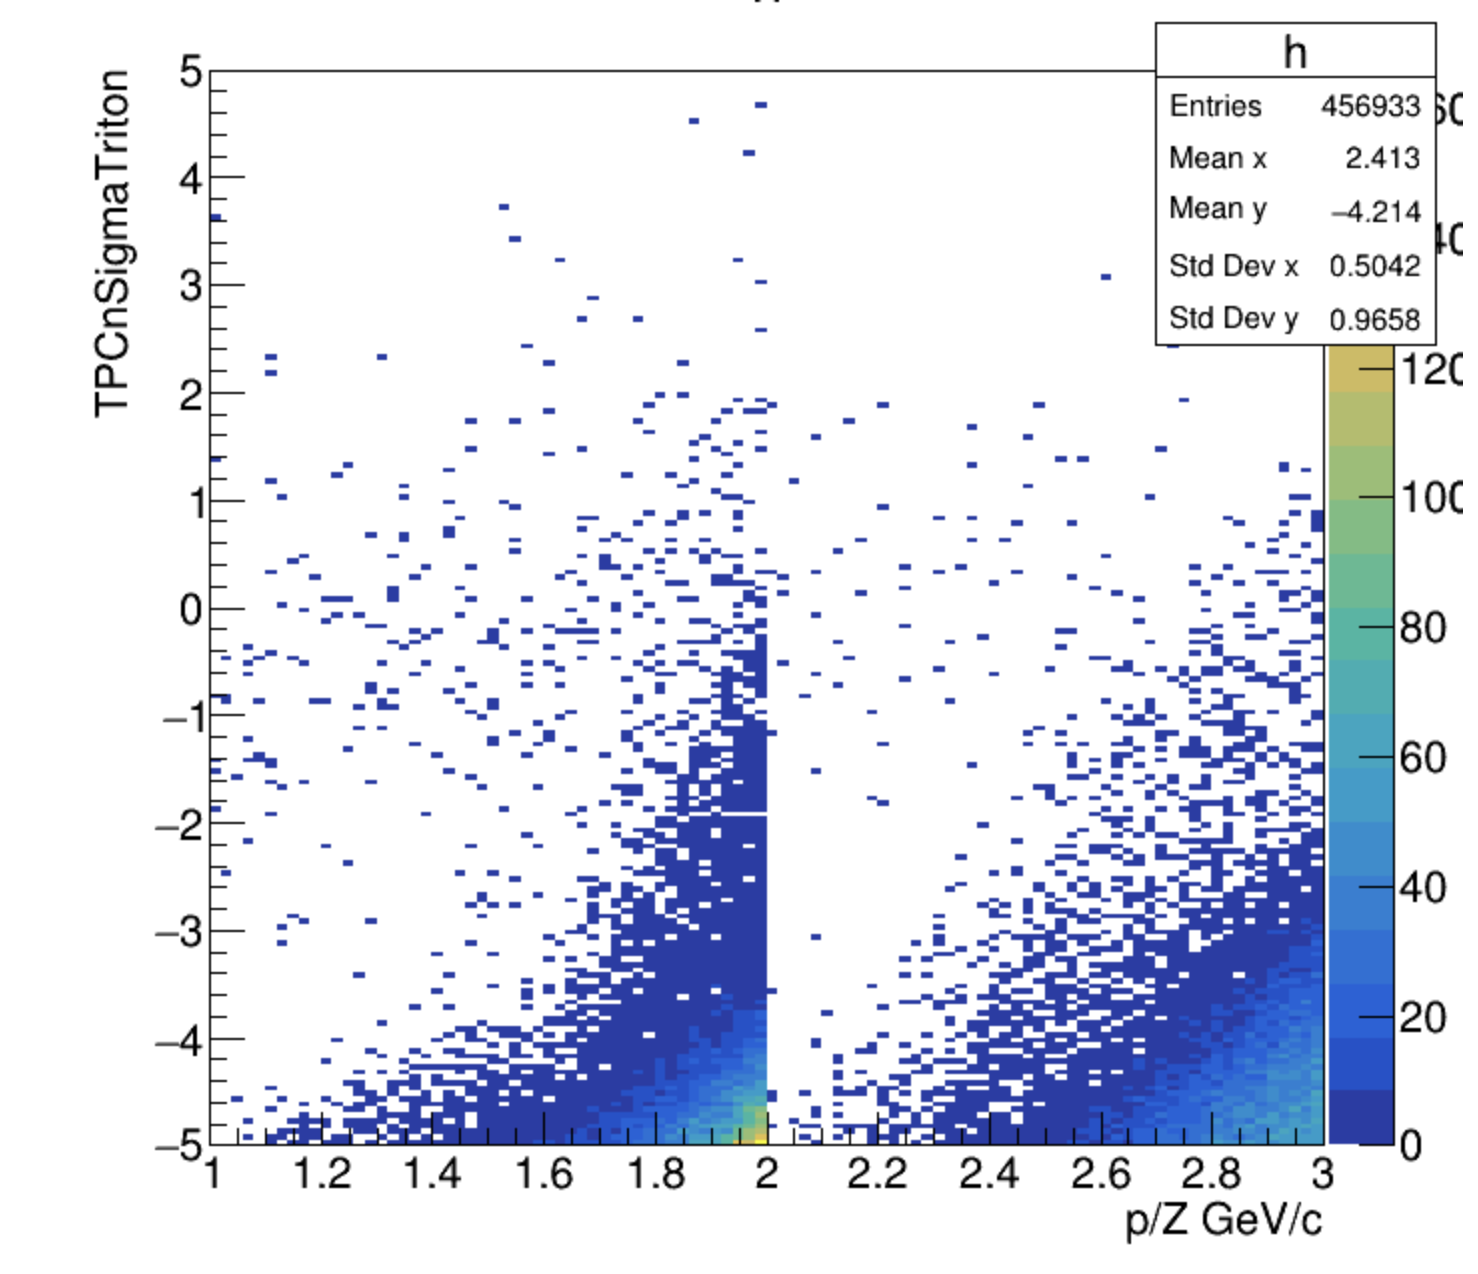
\includegraphics[width=0.48\textwidth]{figures/triton/tbar_TPCnSigma_noTOFcut.png}
    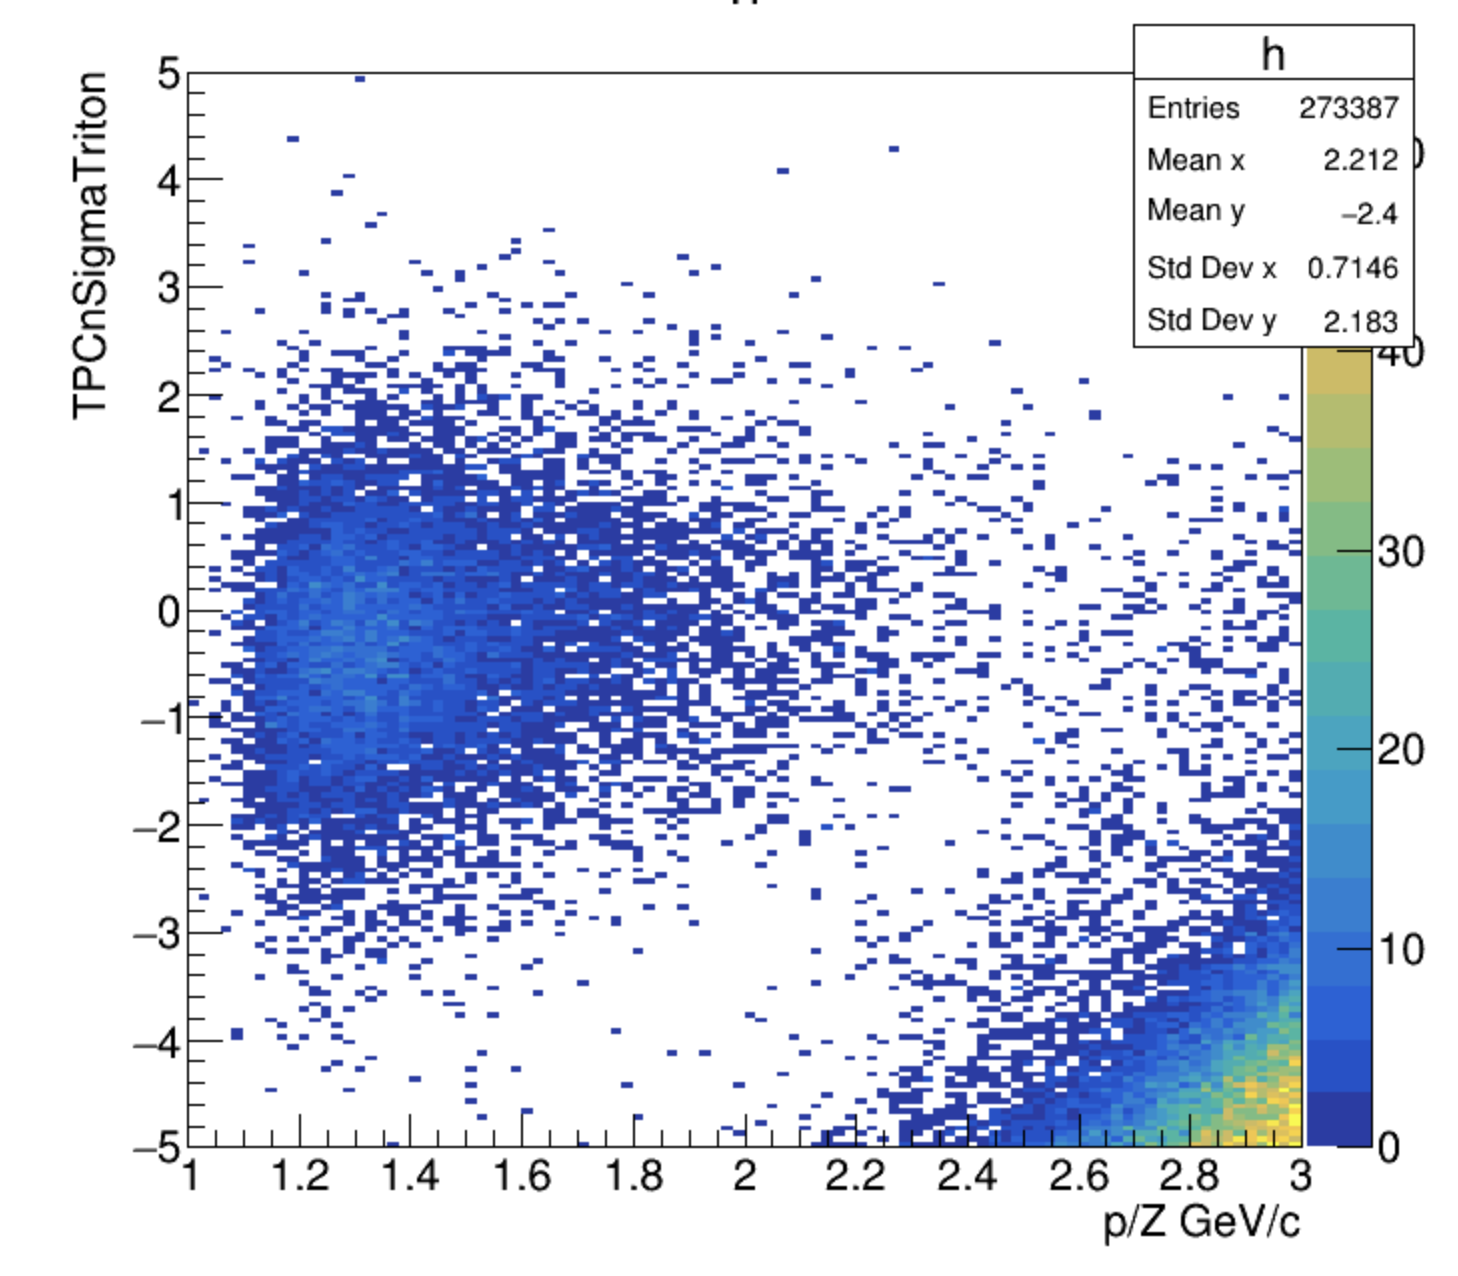
\includegraphics[width=0.48\textwidth]{figures/triton/tbar_TPCnSigma_TOF_cit_noDCA_cut.png}
    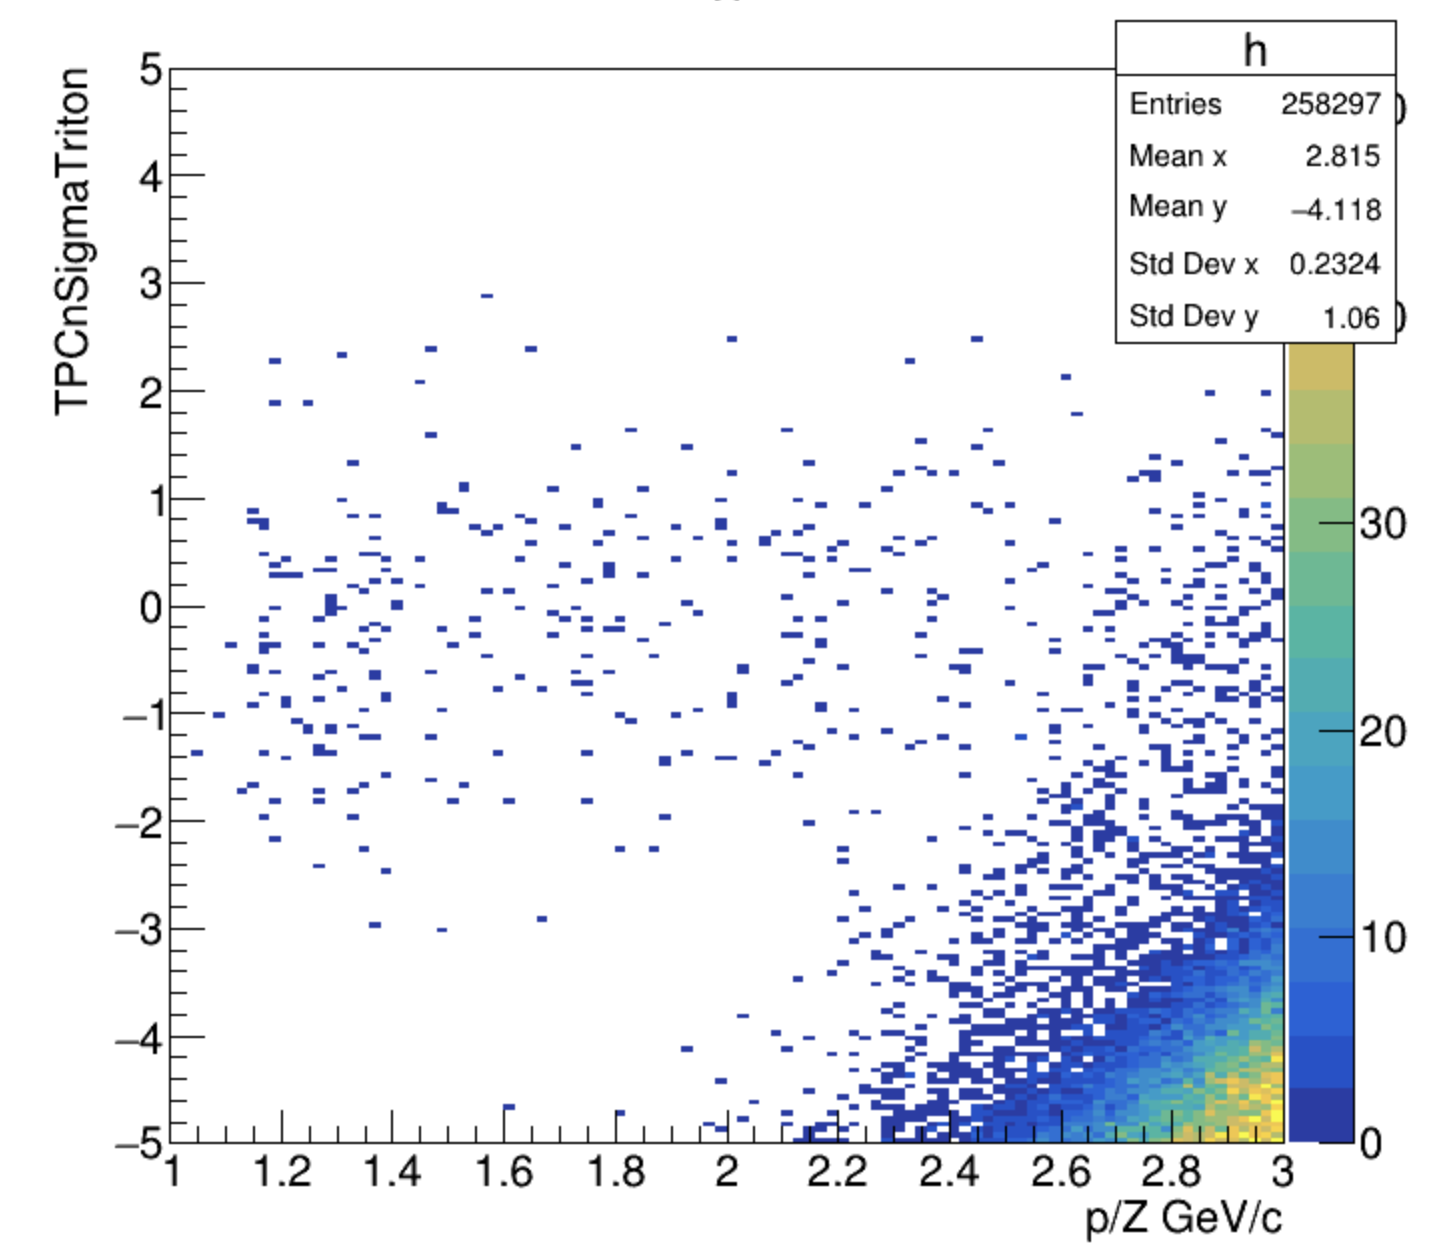
\includegraphics[width=0.48\textwidth]{figures/triton/tbar_TPCnSigma_TOF_cut_and_DCA_cut.png}
    \caption{$n\sigma_{\mathrm{TPC}}$ vs momentum plots for tritons. A cut on the $m_{\mathrm{TOF}}$ is applied above 2 GeV/$c$ in all figures. (Top left) the original distribution without an additional cut on either DCA or $m_{\mathrm{TOF}}$. (Top right) the distribution after a cut of $|\mathrm{DCA}_{xy}|<1\ mm\ \textrm{and}\  |\mathrm{DCA}_z|<1\ mm$ is applied. (Bottom left) the distribution after the cut on $m_{\mathrm{TOF}}$ is extended to momenta as low as 1 GeV/$c$. (Bottom left) the distribution after both the DCA and $m_{\mathrm{TOF}}$ cuts were applied.}
    \label{fig:Tritons_momentum_range}
\end{figure}
Due to the single charge of \atrit\ , there are a few noteworthy differences in the particle identification in comparison to \ahe\ . The first and most important difference is that it is not clearly identifiable in the TPC alone at high momenta. This can be seen in figure \ref{fig:PID_TPC}, which shows that the expected energy loss for (anti)$^3\mathrm{H}$ merges with the bands from other particles at about 1.5 GeV. The considerations for the identification are shown in figure \ref{fig:Tritons_momentum_range}, which shows how the TOF cut is able to remove the contamination up to a momentum of $\approx$ 2.4 GeV/$c$, while the DCA cut removes much of the secondary contribution at low momentum. Additionally, by comparing the top and bottom panels on the right side of figure \ref{fig:Tritons_momentum_range}, which show the effect of the TOF cut after the DCA cut is applied, we can see that the additional requirement of the TOF removes all the contamination at low momentum, while preserving a large fraction of the signal. Furthermore, the fact that the the TOF is required means that the particles have to traverse more material, and thus the ratio becomes more sensitive to the inelastic cross section. Thus, the TOF is used in the whole momentum range for the measurement of the \atrit\ /$^3\mathrm{H}$ ratio. 


\subsection{Secondary correction}
\begin{figure}
    \centering
    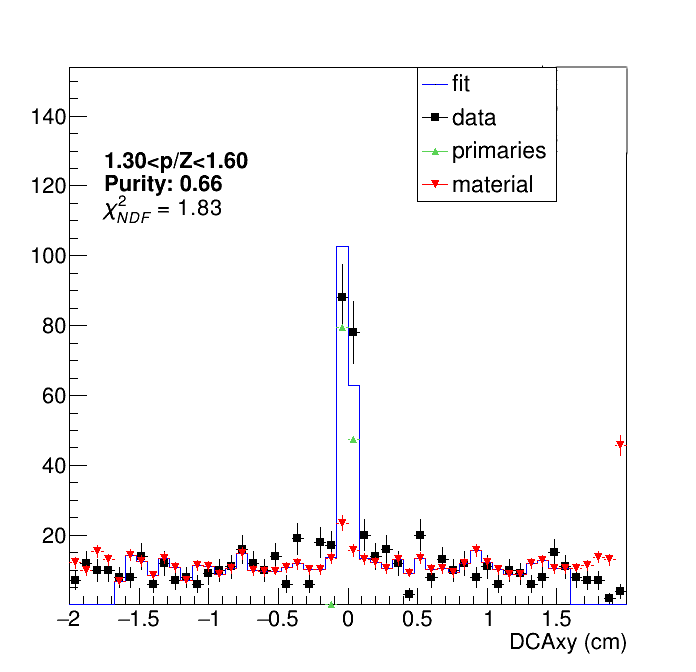
\includegraphics[width=0.32\textwidth]{figures/triton/Templates/TemplateFitHe3_1.3<p<1.6_rebin_2_Bin_1.png}
    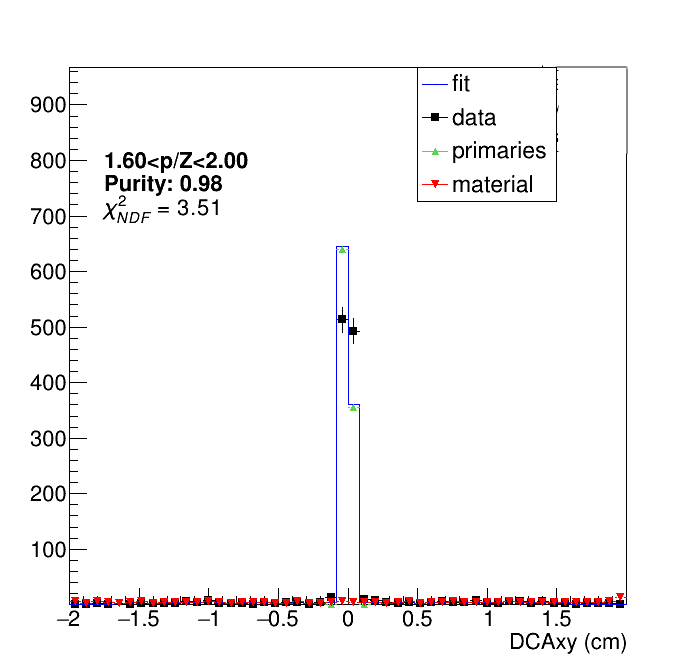
\includegraphics[width=0.32\textwidth]{figures/triton/Templates/TemplateFitHe3_1.6<p<2_rebin_2_Bin_2.png}
    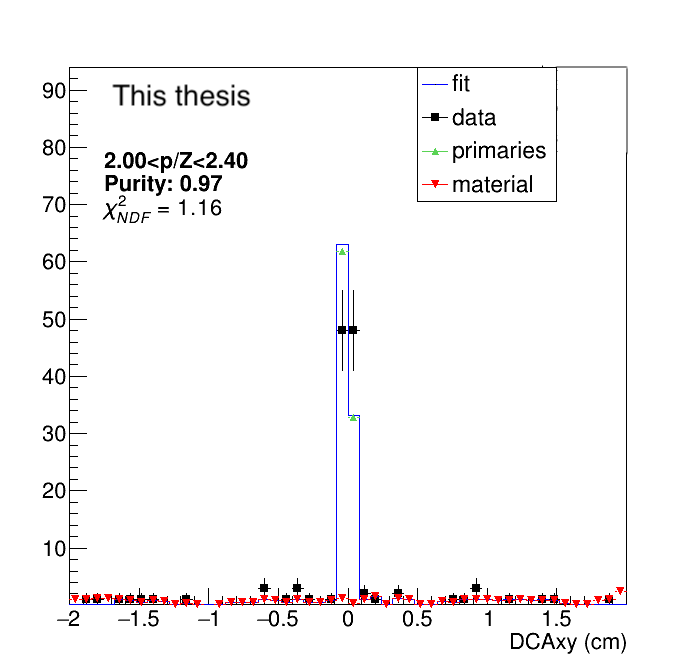
\includegraphics[width=0.32\textwidth]{figures/triton/Templates/TemplateFitHe3_2<p<2.4_rebin_2_Bin_3.png}
    %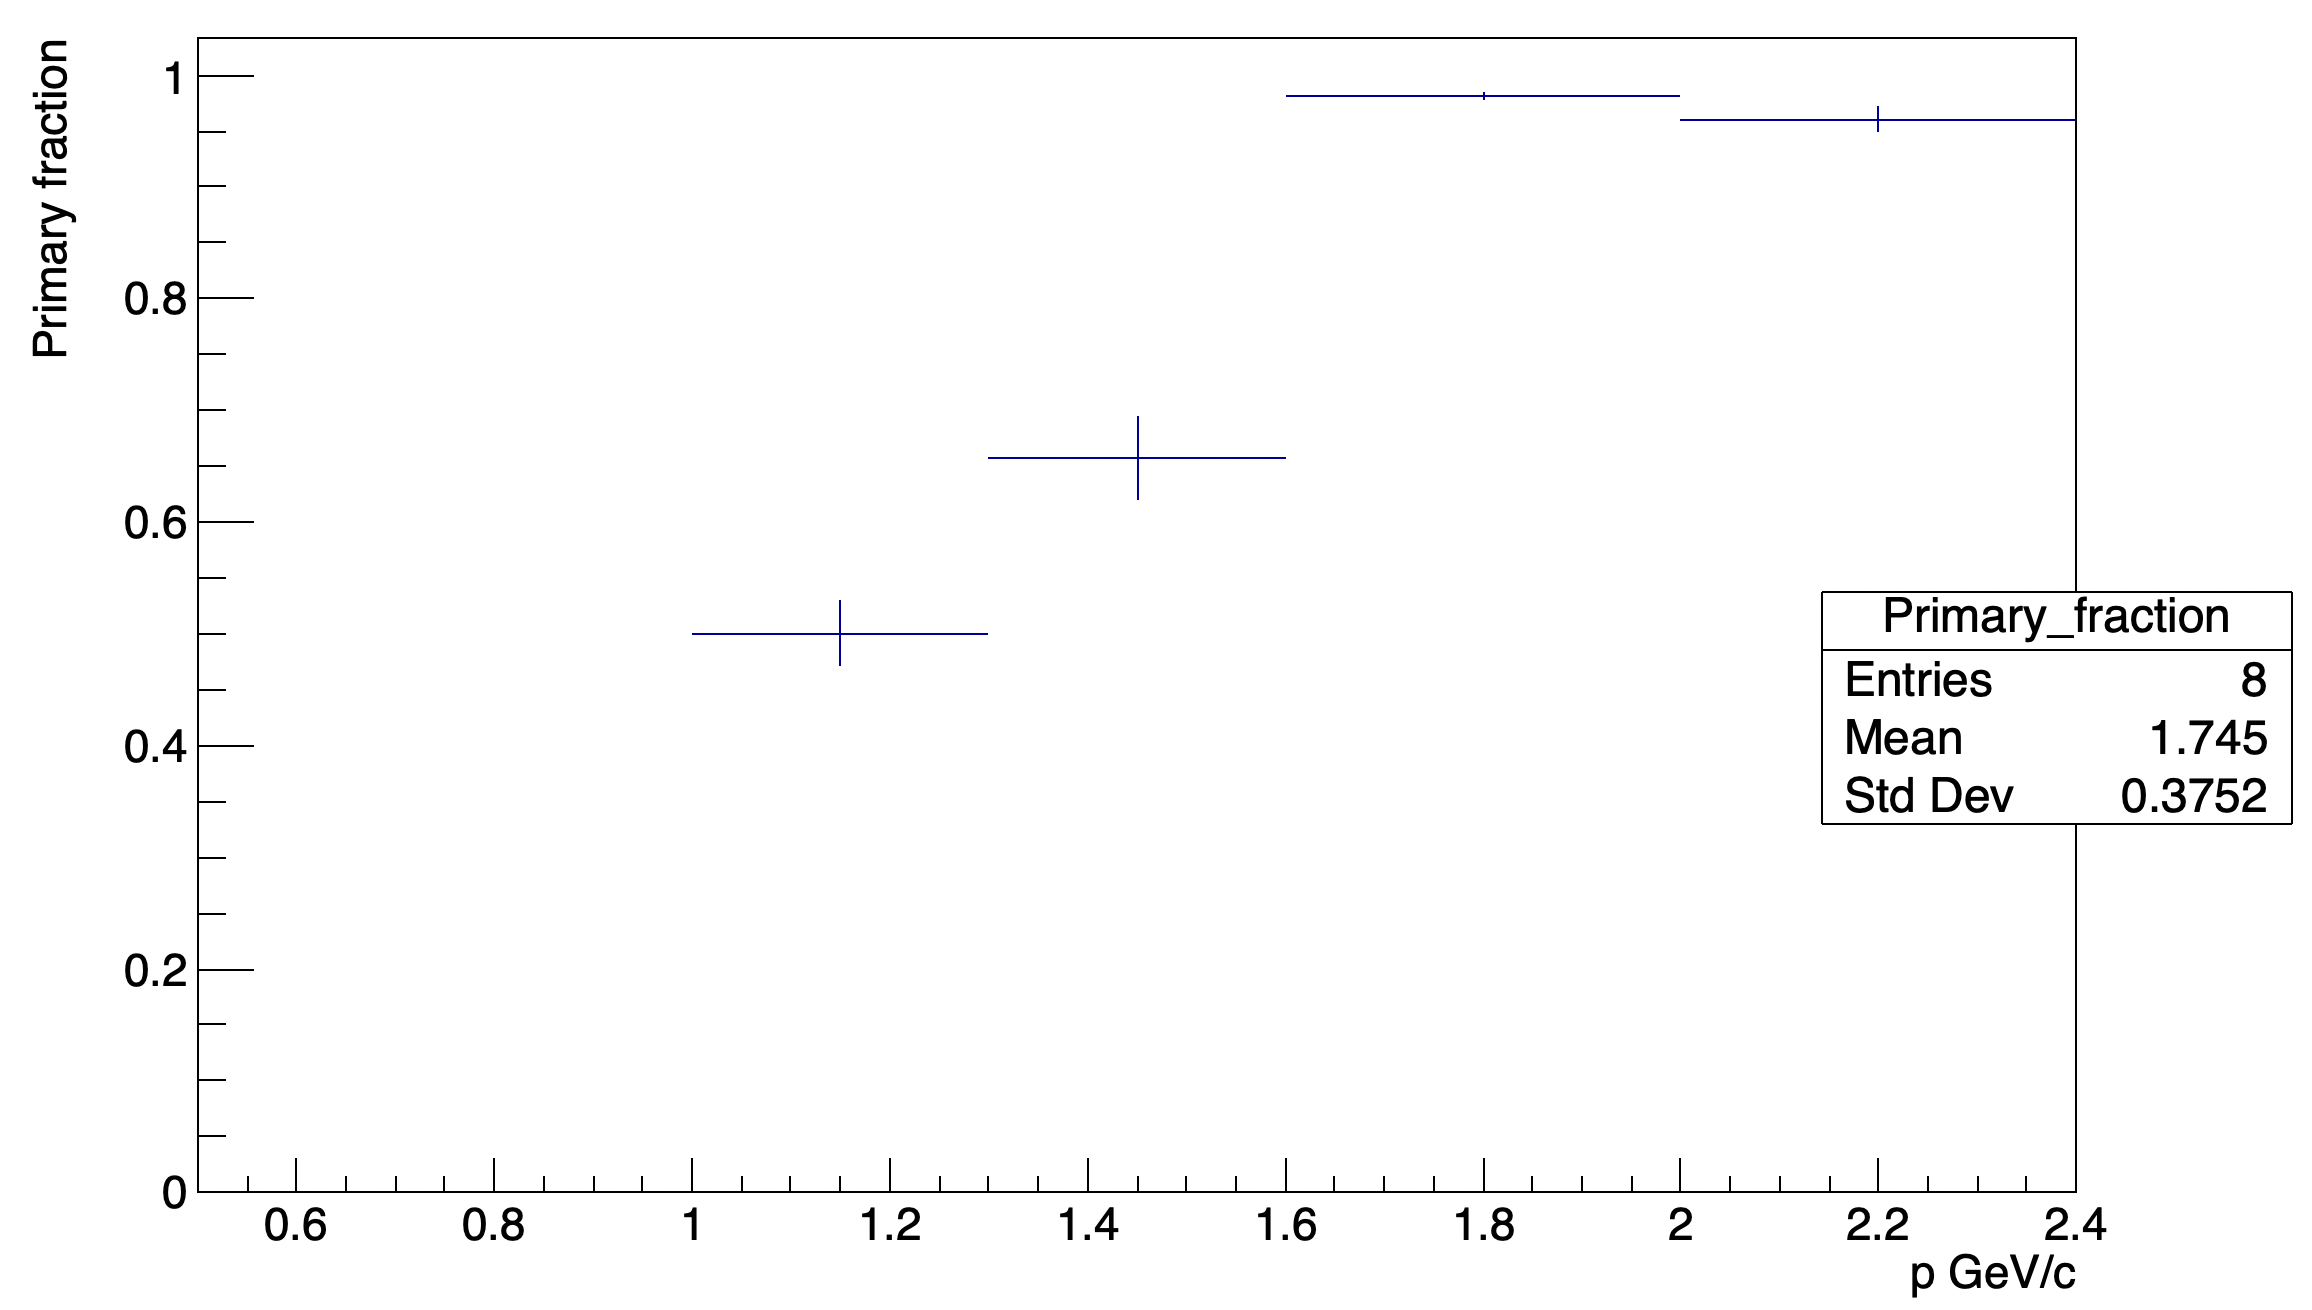
\includegraphics[width=0.75\textwidth]{figures/triton/tbar_Primary_fraction.png}
    \caption{Template fits to the DCA distribution of $^3\mathrm{H}$, to account for the contributions from secondary nuclei from spallation processes. The primary fraction is evaluated as $f_p = \int_{-0.1cm}^{0.1cm} \mathrm{fit}_{\mathrm{signal}} d\mathrm{DCA} / \int_{-0.1cm}^{0.1cm}\ \mathrm{data}\ d\mathrm{DCA}$. The results are shown for each momentum bin.}% (Bottom row) The resulting primary fraction of $^3\mathrm{H}$ in pp collisions at $\sqrt{s}=13$ TeV.}
    \label{fig:TemplateFitsTriton}
\end{figure}
Similarly as for \ahe\ , the \atrit\ /$^3\mathrm{H}$ ratio still needs to be corrected for the remaining secondary nuclei from material spallation. This is done using template fits, according to the method described in \ref{sec:Meth:secondaryCorr}. The fits are shown in figure \ref{fig:TemplateFitsTriton}. It can be seen that the contribution is negligible in the second and third bin. In the first bin, the contribution from secondaries is well constrained. The resulting primary fraction is shown in the bottom of the figure. The uncertainty of the primary fraction is added to the systematic uncertainties on the \atrit\ /$^3\mathrm{H}$ ratio in quadrature.


\subsection{Results}
In this section, the measurements of \sigmainelH\ are presented. The left side of figure \ref{fig:Results:tbar:ratios} shows the \atrit\ /$^3\mathrm{H}$ ratio as measured in pp collisions, and the left side of figure \ref{fig:Results:tbar:xs} shows the resulting inelastic cross section measurement with the open circles. The measurement is consistent with the parameterization used in Geant4 within a significance of 2 $\sigma$, but shows a hint at a systematically larger vale for \sigmainelH\ . The right side of figure \ref{fig:Results:tbar:ratios} shows the TOF/TPC ratio of \atrit\ in Pb -- Pb collisions at $\sqrt{s_{\rm{NN}}}=5.02$ TeV\footnote{These were not obtained as part of this thesis, but were obtained for the same publication as the cross section in Pb--Pb collisions (publication is in preparation).} and the corresponding measurement of \sigmainelH\ is shown on the left of figure \ref{fig:Results:tbar:xs} as full circles. The measurements are compared with the results for \ahe\ in the right panel of figure \ref{fig:Results:tbar:xs}, all scaled to the same average material, which shows that the results for \atrit\ and \ahe\ are consistent within uncertainties. This means that within the current uncertainties, the annihilation cross sections are consistent with isospin symmetry. Improvements on the statistical precision of these measurements will help constrain this assumption further using the data from the upcoming Run 3 and Run 4 campaigns at the LHC. 

\begin{figure}
    \centering
    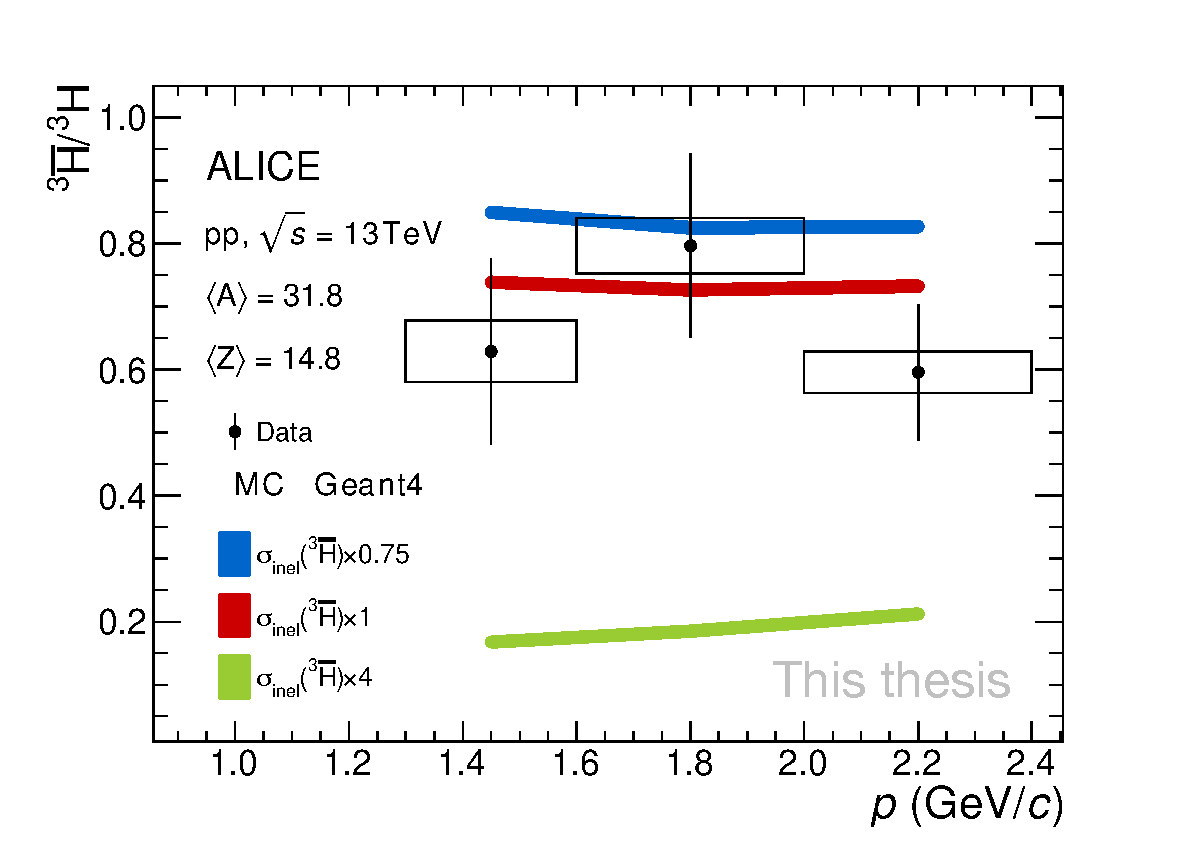
\includegraphics[width=0.48\textwidth]{figures/Anti-triton-to-triton_Ratio.pdf}%pp ratio plot
    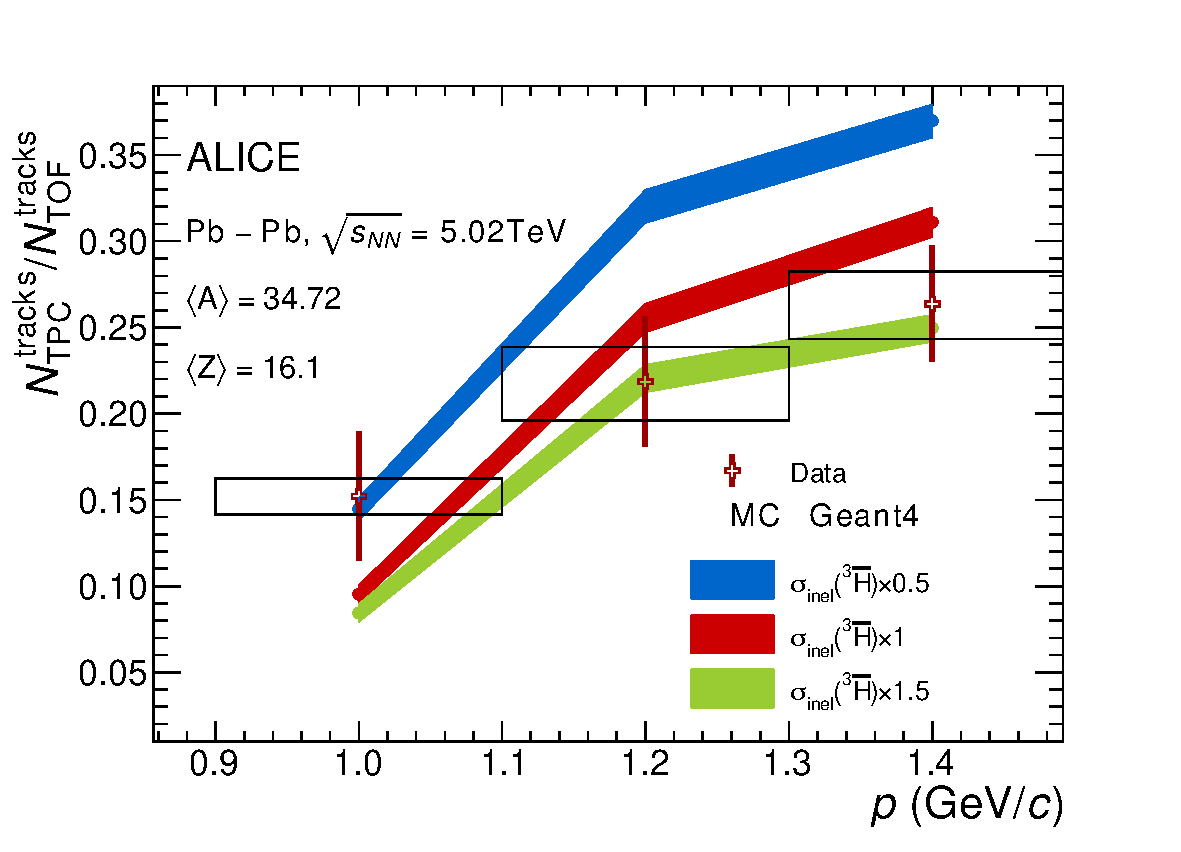
\includegraphics[width=0.48\textwidth]{figures/Anti-triton-TPC-TOF_Ratio.pdf}%sigma inel in pp
    \caption{(Left) \atrit\ /$^3\mathrm{H}$ ratio as a function of momentum, with statistical uncertainties as bars and systematic uncertainties as boxes. The colored lines represent Monte Carlo simulations with varied inelastic cross sections. (Right) \atrit\ TOF-to-TPC ratio as a function of momentum, with statistical uncertainties as bars and systematic uncertainties as boxes. The colored lines represent Monte Carlo simulations with varied inelastic cross sections. }
    \label{fig:Results:tbar:ratios}
\end{figure}

\begin{figure}
    \centering
    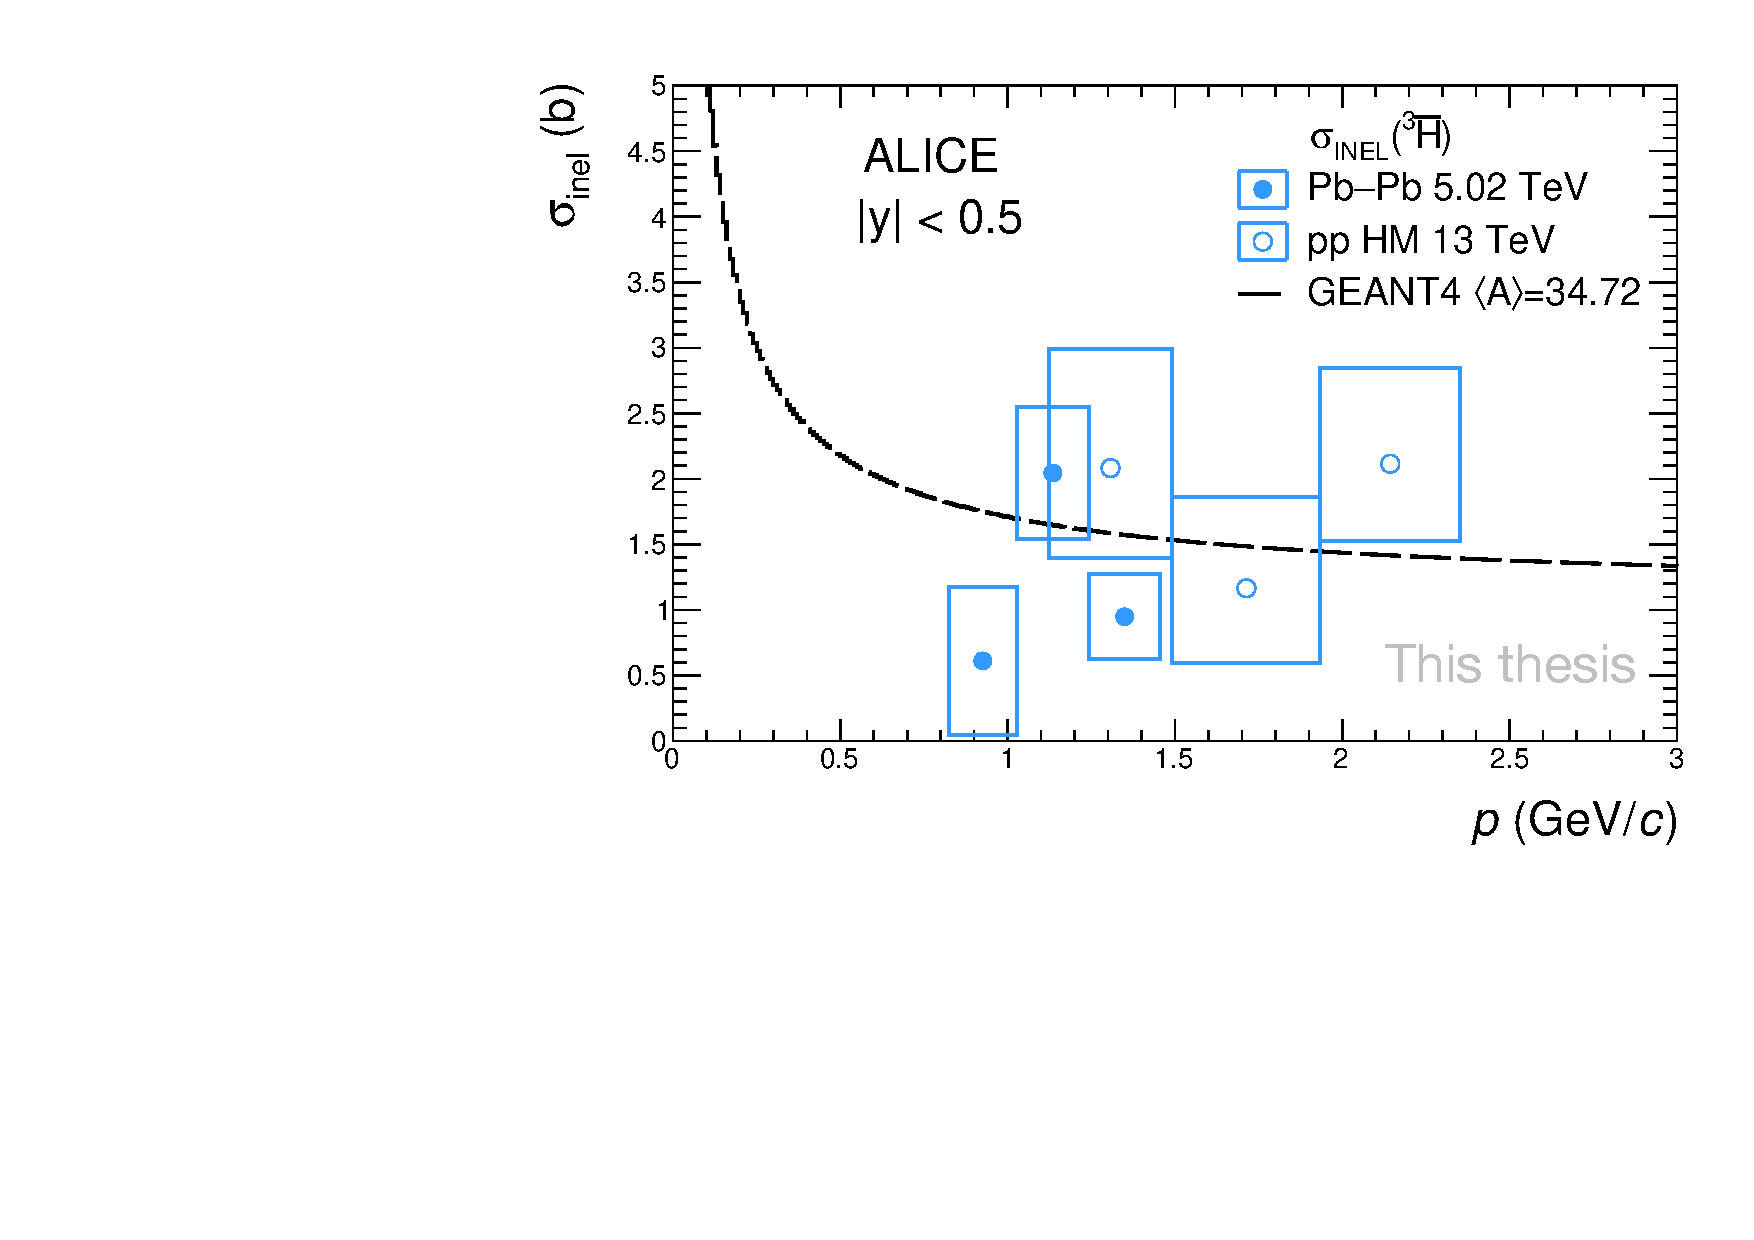
\includegraphics[width=0.48\textwidth]{figures/FinalXS_antit_paper.pdf}%PbPb ratio plot
    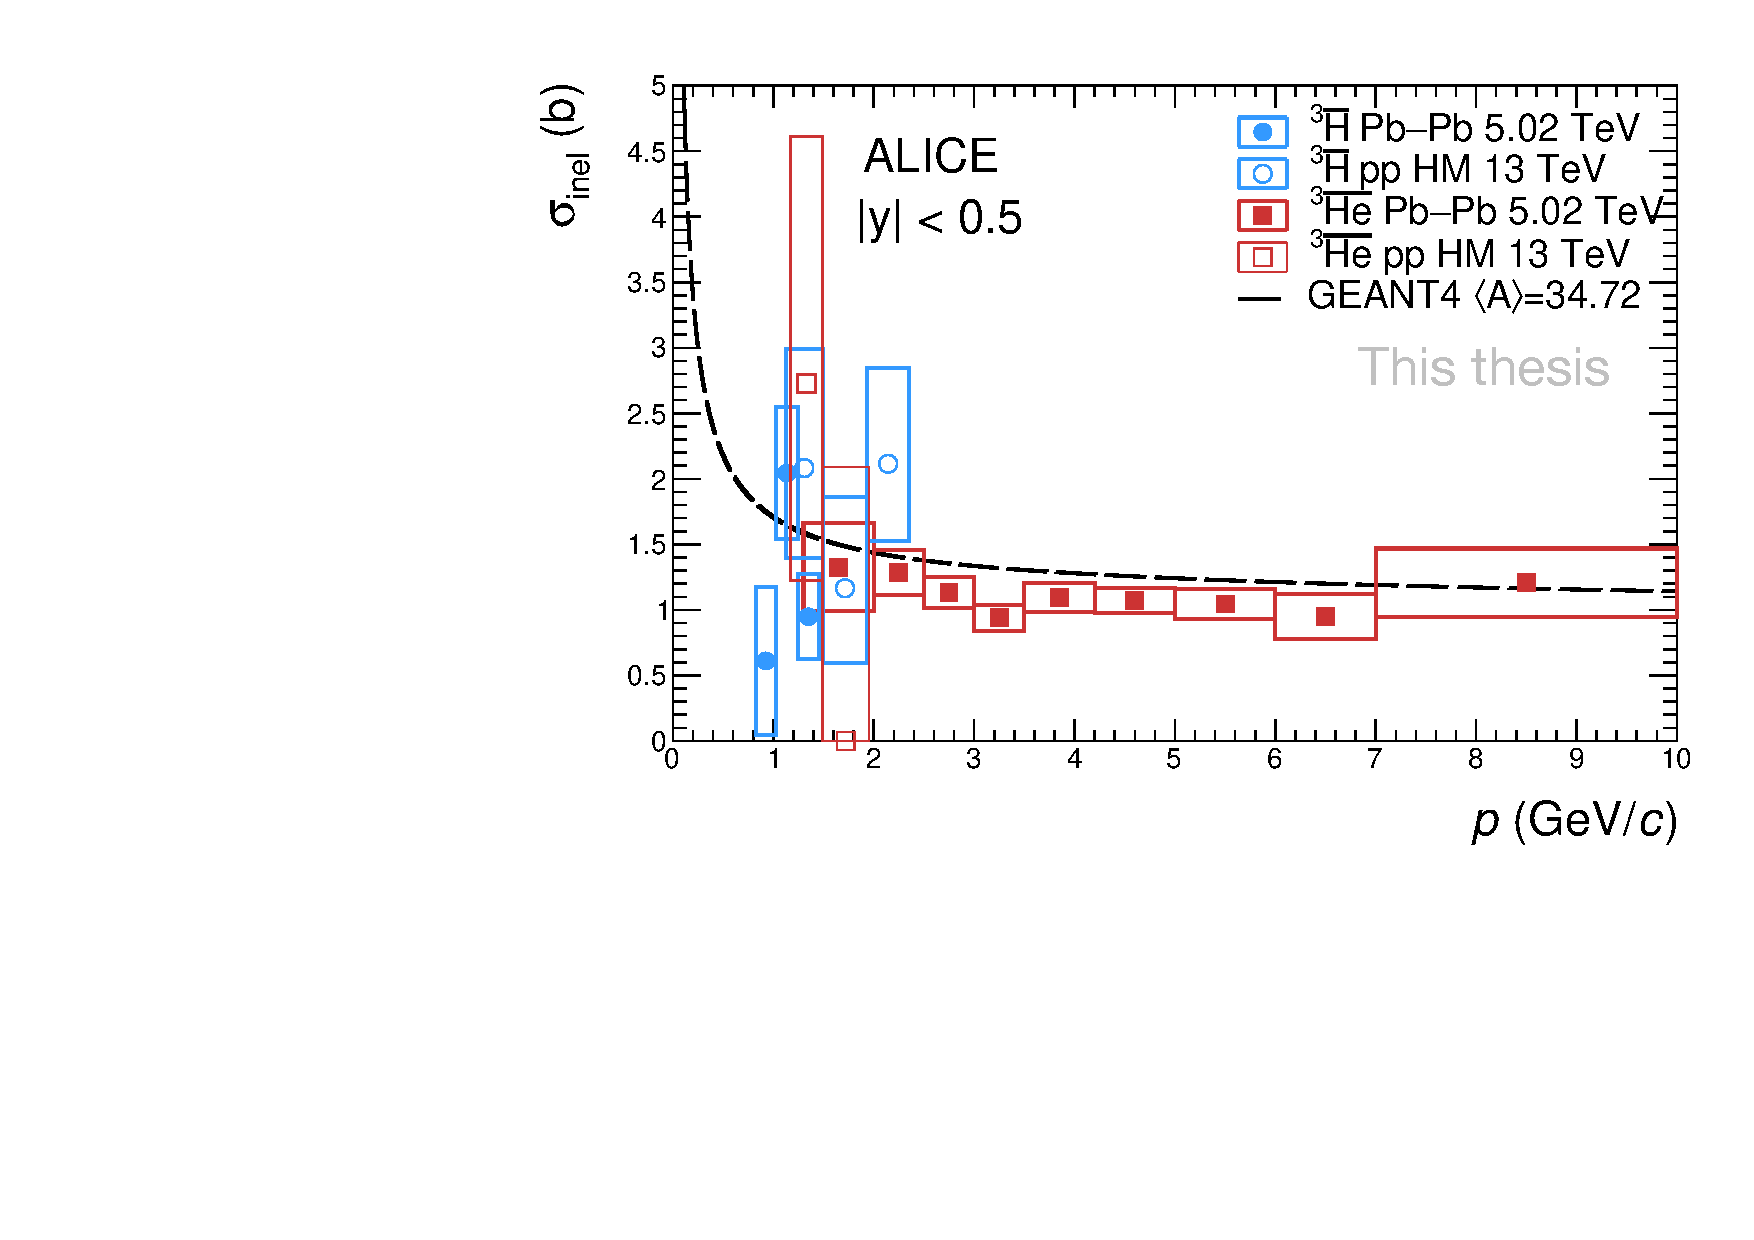
\includegraphics[width=0.48\textwidth]{figures/FinalXS_antitantiHe3_paper.pdf}%sigma inel PbPb
    \caption{(Left) the resulting measurement of \sigmainelH\ using the antibaryon-to-baryon method ($\mathrm{\overline{B}}/\mathrm{B}$) and the TOF-to-TPC method, on the average ALICE material. The colored boxes show the total uncertainty (stat$^2 +$ syst.$^2$). The line shows the parameterization as used in Geant4. (Right) comparison of the \sigmainel\ and \sigmainelH\ measurements.}
    \label{fig:Results:tbar:xs}
\end{figure}


\newpage




\newpage
\section{Antinuclei in the cosmos}\label{sec:AntinucleiInTheCosmos}
Antinuclei are some of the rarest stable objects in cosmic rays, in fact, no compound antinuclei have ever been conclusively observed in cosmic rays. But it is this exact fact that makes them such promising candidates for the search of new physics beyond the Standard Model. Whereas for other particle species the signal-to-background ratio might be minuscule for any new effect, antinuclei production is so rare in standard model processes that any new physics might produce signals orders of magnitude greater than what can be explained with our current knowledge. While no conclusive observation of antinuclei in cosmic rays has been published, the AMS-02 Collaboration has repeatedly reported potential signals of antihelium \cite{AMS_ahe_report, AMS_ahe_tease, MIAPP_AMS_dbar}, motivating a renewed push of research interest into cosmic-ray antinuclei. \\

\begin{figure}
    \centering
    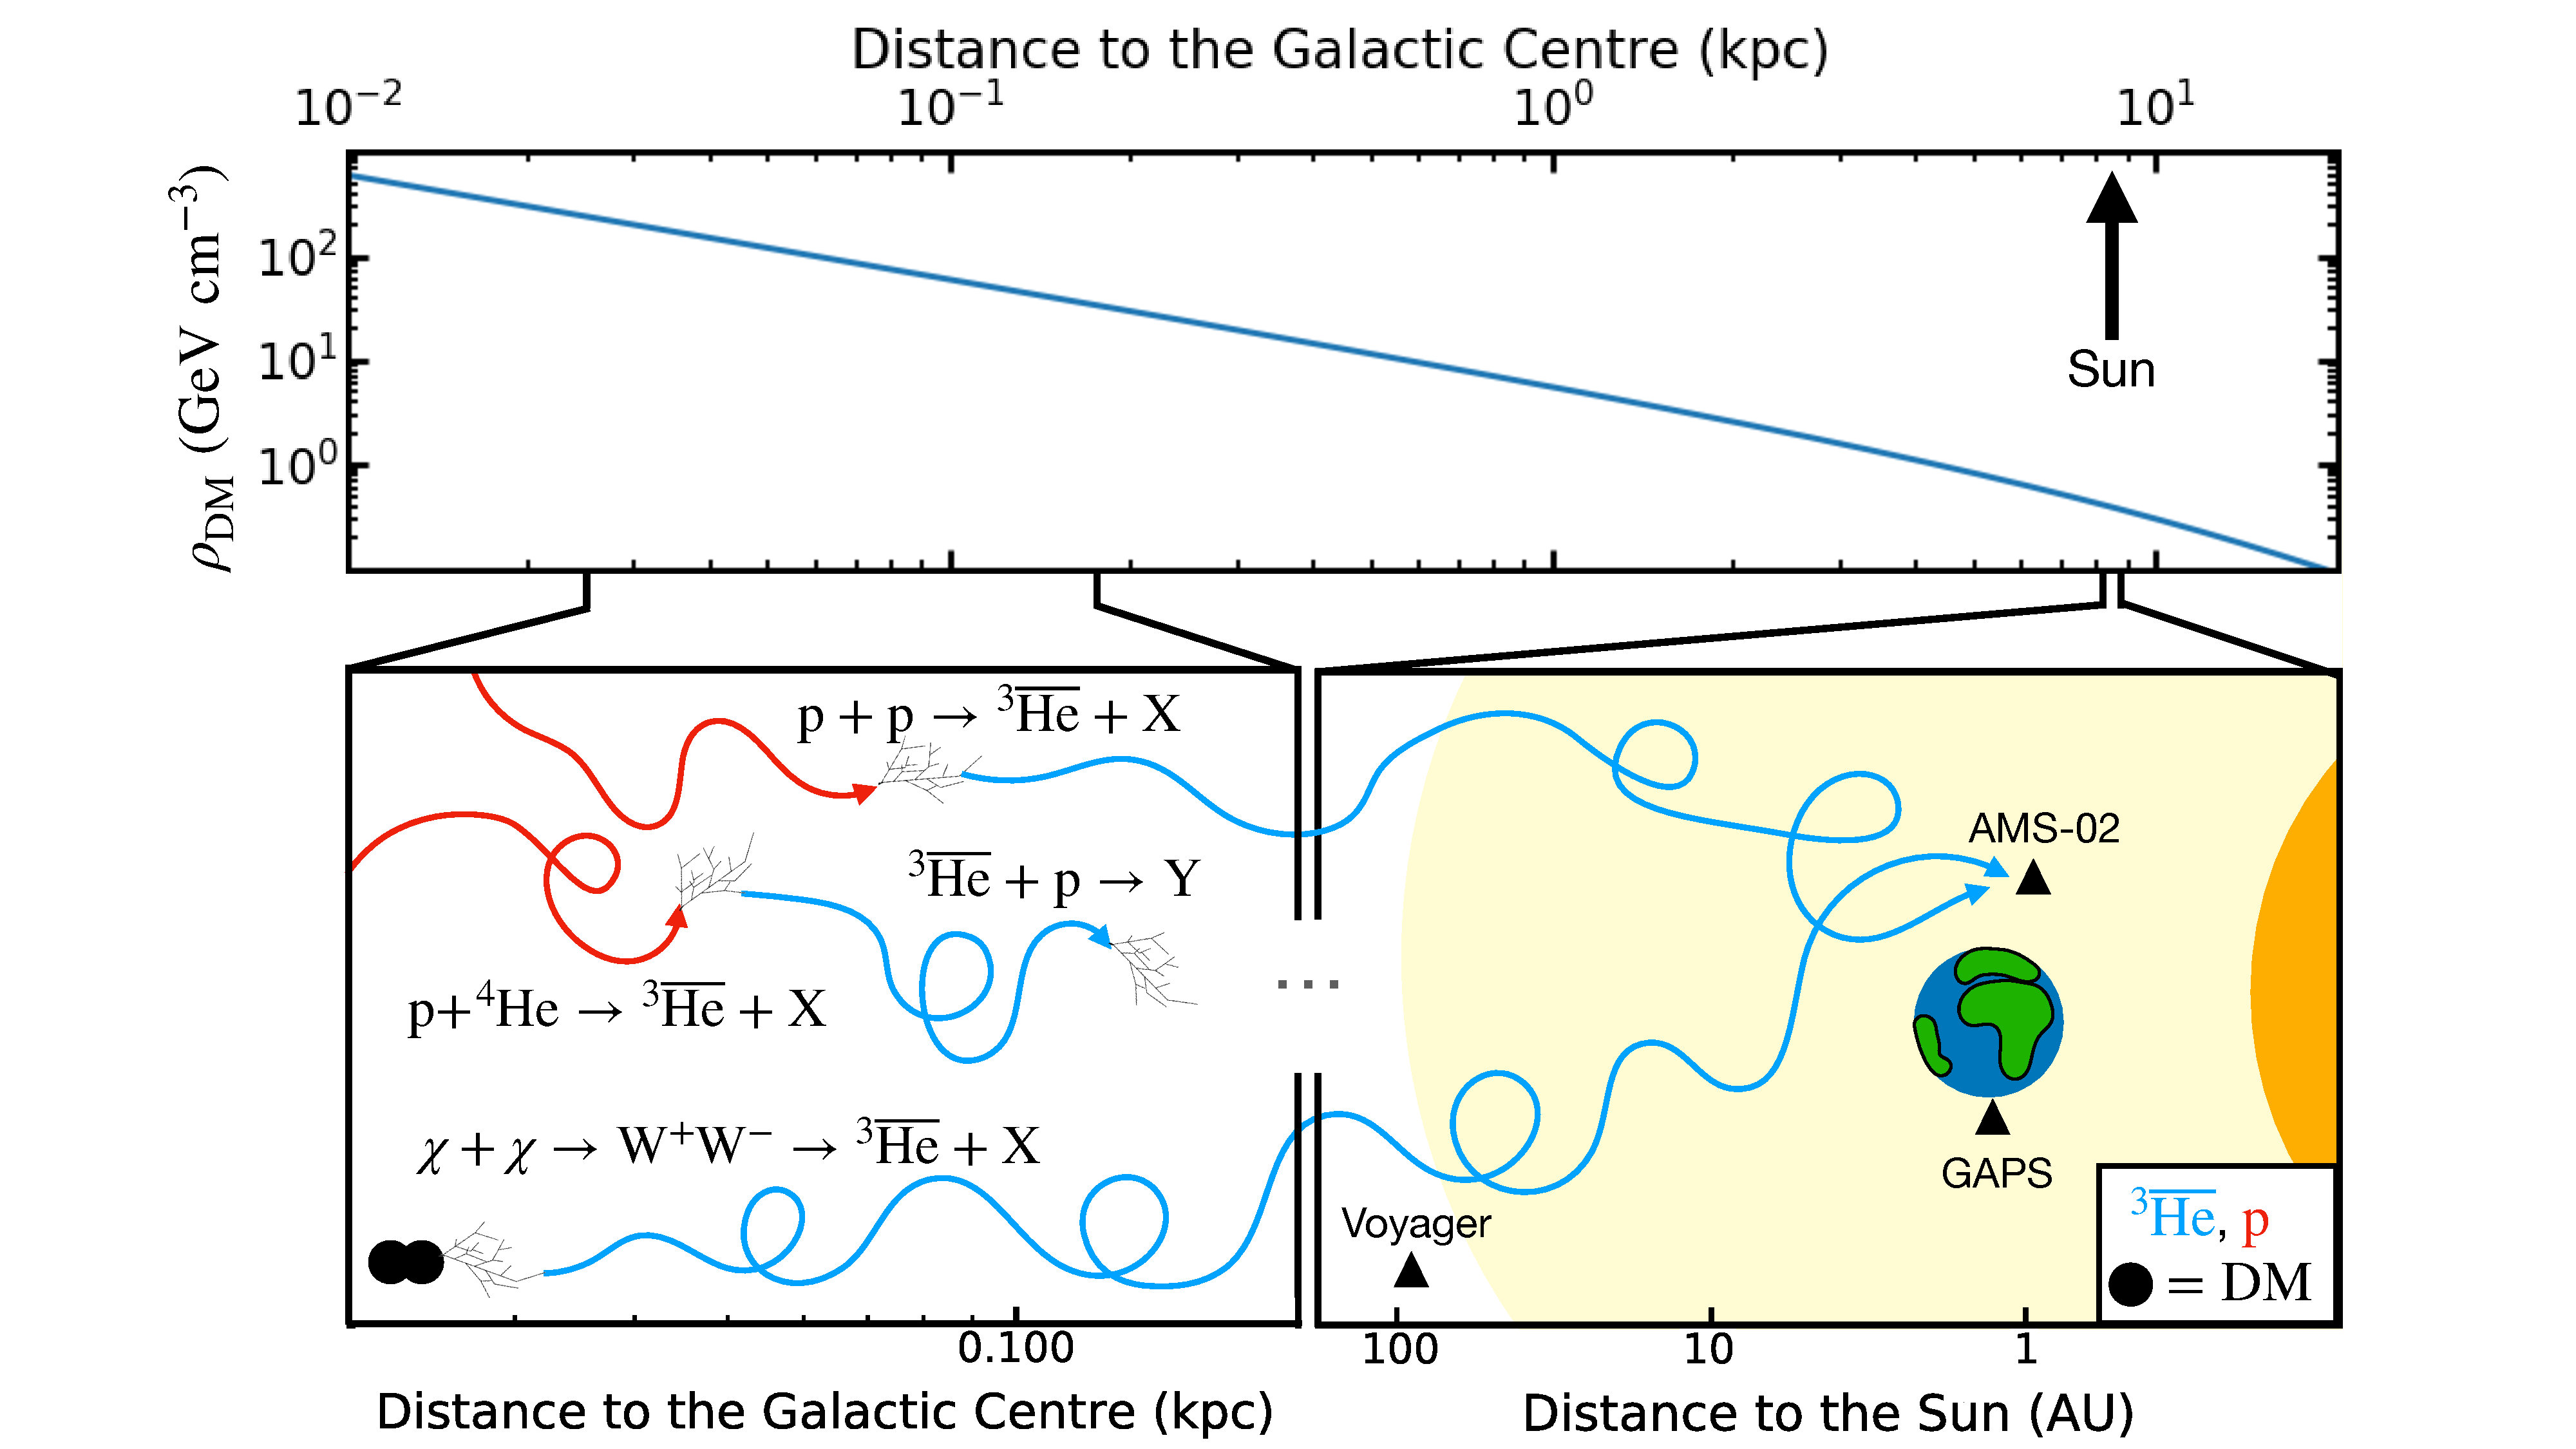
\includegraphics[width=\textwidth]{figures/GalaxyStory.pdf}
    \caption{Illustrated story of the journey which antinuclei undertake before being observed near earth. Red lines shown high energy cosmic ray protons, Blue lines shown \ahe\ . The antinuclei get created all throughout the galaxy, and in the galactic centre antinuclei from dark matter is the most concentrated, due to the higher dark matter density. Similarly, antinuclei from high energy cosmic rays are created all over the galaxy. The created antinuclei then travel through the interstellar medium, some of them annihilating along the way. The ones which do make it to earth then are affected by the solar magnetic field, before reaching detectors near earth. All these processes need to be understood in order to be able to interpret an antinuclei signal in cosmic rays.}
    \label{fig:Galaxy_story}
\end{figure}
The goal of this section is to discuss possible exotic sources of antinuclei in our galaxy focusing on WIMP dark matter and extragalactic WIMP dark matter. For antideuterons primordial black holes are also discussed as a possible source. These are compared to antinuclei produced in high-energy cosmic-ray collisions with the interstellar medium, which in the respective rest frame is an analogous process to the one used to produce antinuclei at accelerators. In the lab frame the collision is heavily boosted, which affects the produced spectra. Crucially, the new measurements of the inelastic cross sections of antihelium laid out in Section \ref{sec:ResHe3SigmaInel}, and the first low-energy measurements of the antideuteron--matter inelastic cross section laid out in \cite{antideuteronXS}, are for the first time incorporated in such studies. The discussion therefore focuses in particular on propagating these measurements to obtain the experimental uncertainites from inelastic interactions on the antinuclei flux near earth. This journey from creation to observation for antinuclei is illustrated in figure \ref{fig:Galaxy_story}.\\


In order to study the two sources we employ the GALPROP framework \cite{Galprop_propagation}. This framework propagates particles through our galaxy, simulating various effects such as diffusion, convection and also inelastic processes. The resulting fluxes near earth are then presented for both antideuterons and \ahe, for different dark matter masses and profiles. Finally, current and planned experiments for detecting antinuclei in cosmic rays are discussed. 
The antinuclei fluxes from high-energy cosmic-ray collisions shown in this thesis as comparisons to the fluxes from possible dark-matter sources are taken from \cite{Serksnyte:2022onw} and \cite{ALICE-PUBLIC-2022-001}, for antideuteron and \ahe\ respectively.\\




\subsection{Sources of antinuclei in the cosmos}
Antinuclei are some of the rarest stable particles in our galaxy, since very few abundantly occurring processes will produce them in any detectable amount \cite{Poulin_AMS_ahe_events, Coogan_2017}. This is in contrast to nuclei, which are the most abundant stable particles within our galaxy. Indeed, nuclei up to Iron have been observed by a variety of methods: in the spectral lines of stars, in cosmic rays by the AMS collaboration \cite{AMS_B_to_C} and of course on earth. A large amount of the light matter nuclei (up to Lithium) was produced during Big Bang Nucleosynthesis (BBN) \cite{PDG2022}, while all heavier nuclei were produced during stellar nucleosynthesis \cite{stellar_evo_nucleosynthesis}. This process involves fusing hydrogen nuclei to create the necessary energy inside a star to counteract its own gravitational pull, creating helium in the process. This continues for most of the lifetime of the star, until its reserves of hydrogen run low. Without the sustained temperature and pressure provided by hydrogen fusion, the star's core will become inert and contract under gravity. Meanwhile, fusion will start in the outer layers of the star, where residual hydrogen is still found. This causes those layers to expand and cool, and the star forms what is called a red giant \cite{stellar_evo_nucleosynthesis} or red supergiant \cite{stellar_evo_nucleosynthesis}. Over time, the core will contract and heat up\footnote{Red supergiants may have sufficient pressure immediately to commence helium fusion in their core. For more information on stellar information please refer to \cite{stellar_evo_nucleosynthesis}.}, until the conditions allow for even heavier elements (helium and sometimes carbon) to start fusing to create energy \cite{stellar_evo_nucleosynthesis}. During this process, elements up to iron are created through nuclear fusion, and heavier elements can be created through slow neutron capture processes \cite{stellar_evo_nucleosynthesis}. This process accounts for the production of roughly half of the elements heavier than iron \cite{stellar_evo_nucleosynthesis}. When this source of energy becomes insufficient, the red giant's will implode and expel its outer shell, creating a planetary nebula. Red supergiants will explode in a supernovae, expelling huge amounts of energy and matter. In this process, rapid neutron capture occurs, producing the other half of elements heavier than iron \cite{Supernovae_nucleosynthesis}. \\
However, due to the asymmetry of matter and antimatter in our galaxy, neither BBN nor stellar nucleosynthesis is thought to be a dominant source for antinuclei. Antimatter produced during BBN is likely to have annihilated propagating through the galaxy from the Big Bang until today. This can be shown by a back of the envelop calculation. Assuming an antinucleus with an annihilation cross section of $\approx$1b and a momentum of $\gtrapprox$ 0.1 GeV/n, the fraction surviving until this day is given by $N/N_0 = \mathrm{exp}(-\sigma n \beta c t)$, where $n$ is the average matter density in the regions traversed. Taking $n = 1 \mathrm{cm}^{-3}$ and using $\beta = p/\gamma m$ one finds that only about $e^{-100} \approx 10^{-44}$ of the initial population would still be left today.  And in order for stellar antinucleosynthesis to occur, anti-starts -- or at least large clouds of antimatter -- would have to exists. Any such regions would by default have to come in come in contact with the matter dominated regions which predominantly make up our galaxy. In those overlap regions, significant amounts of annihilations would cause a visible gamma ray signal \cite{Poulin_AMS_ahe_events}.  No signal of this kind has been reported, although if such regions were small enough, they would appear as point sources to current instruments and thus make up a part of the currently unidentified point sources within our galaxy \cite{FermiLAT_Point_Sources}. Recent work has claimed that such antimatter regions may have formed during the big bang and survived to this day \cite{DM_gamma_rays, Gamma_DM_searches}, making up $\approx$ 20 of the roughly 1000 unidentified point sources. However, these studies also note the necessity for the antimatter regions to have formed in places where the proton density is O($10^{-8}$) of the cosmic average.  The authors do not provide a viable mechanism by which this could have occurred. \\
We therefore have to look to other processes which could produce antinuclei. Due to baryon number conservation, all such processes are likely to produce at least an equal amount of light nuclei as well. However, since nuclei are far more abundant than antinuclei, these processes will only contribute a negligible amount to the total nuclei flux in our galaxy, while they might dominate the antinuclei flux. This extremely high expected signal-to-background ratio is the reason why antinuclei are considered such a promising probe into new physics.

\subsubsection{High-energy cosmic-ray collisions}
The most well-known source for antinuclei in cosmic rays --- and the only one which does not require new physics or as of yet undiscovered objects --- are collisions of high-energy cosmic rays with the interstellar medium. Such collisions, akin to collisions at particle accelerators, will produce antinuclei by converting the available mass--energy from the collision into (anti)nucleons which then coalesce (see section \ref{sec:IntroProductionAntinuclei} for a more detailed discussion on antinuclei production).  In order to predict the production of antinuclei in such high energy collisions we need to know the differential production cross section of the antinuclei in question, for each collision which can occur, and we need to know which collisions those are, i.e. we need to know the composition of cosmic rays and of the interstellar medium, as a function of energy. For both the interstellar gas and cosmic rays, the composition is $\approx$90\% protons, $\approx$9\% Helium-4 and $<$1\% heavier nuclei. Thus, the source term for nuclei from such secondary collisions can be written as 

\begin{equation}\label{eq:secSourceTerm}
    q (\vec{r}, p) = \sum_{CR=\mathrm{H}, \mathrm{He}} \sum_{ISM=\mathrm{H},\mathrm{He}} n_{ISM}(\vec{r} \int dp_{\mathrm{CR}}' \beta_{\mathrm{CR}} c \frac{d\sigma(p, p_{\mathrm{CR}}')}{dp} n_{\mathrm{CR}}(\vec{r}, p_{\mathrm{CR}}')
\end{equation}

, where $\sum_{CR=\mathrm{H}, \mathrm{He}} \sum_{ISM=\mathrm{H},\mathrm{He}}$ denote the sums over the particle species in cosmic rays and the interstellar medium, $n_{ISM}(\vec{r})$ is the density of the interstellar gas at a given point, $n_{\mathrm{CR}}(\vec{r}, p_{\mathrm{CR}}')$ is the density of cosmic rays at a given position and energy, and $\frac{d\sigma(p, p_{\mathrm{CR}}')}{dp}$ is the differential production cross section for an antinucleus, as a function of the momentum of the produced antinucleus $p$ and the momentum of the incoming cosmic ray $p_{\mathrm{CR}}'$. The particles in the interstellar medium are considered to be at rest in this calculation, which is a valid approximation since they move at  very low speeds in comparison to the incoming cosmic rays\footnote{Interstellar gas particles can be expected to move at speeds of the order of the rotational velocity of the milky way, which is O(100 km/s) or O($\beta = 10^-4$). This is much lower than the velocity of incoming protons at the threshold for antinuclei production, where O($\beta >0.999$).}. \\

The production cross section of antinuclei in such small collisions systems is suppressed at low energies due to the baryon number conservation, since it is necessary to produce at least 4 (6) new nucleons in order to produce antideuterons (\ahe). The requirement for these additional nucleons means that the threshold of the required COM energy is about $\sqrt{s}_{\mathrm{th}}\approx 6 (8)  m_p$ for antideuterons (\ahe ). Given that the ISM target is at rest, all the energy must come from the incoming cosmic ray particle. This means that the frame of reference of the collision will be highly boosted in comparison to the galactic frame, and that the centre of mass energy will only rise $\propto \sqrt{E_\mathrm{CR}}$. 
In the case of \ahe\ this corresponds to a threshold energy of the incoming proton of $E_p \approx 31$ GeV. In order to estimate these cross sections, Monte Carlo event generators are used to create the proton and neutron spectra and distributions, and coalescence afterburners are then applied in order to estimate the production of antinuclei. In this work, the production cross sections by \cite{Shukla_2020} and \cite{Gomez_Coral_2018} are used, referred to hereinafter as Shukla et. al. For \ahe\, O($10^{11}-10^{12}$) events are needed to get a statistical precision on the \% level on the total yield for a given incoming beam energy \cite{Shukla_2020}. The resulting production cross sections for \ahe\ and antideuterons are shown in figure \ref{fig:CR_production_XS}, where they are shown for a wide array of incoming beam energies. As can be seen, it requires significantly above the threshold energy of $\sqrt{s}=$31 GeV in ordet to produce any significant \ahe\ flux\footnote{It is the lowest energy considered for antideuterons since the same simulations were used to determine both sets of spectra in Shukla et. al.}.

\begin{figure}
    \centering
    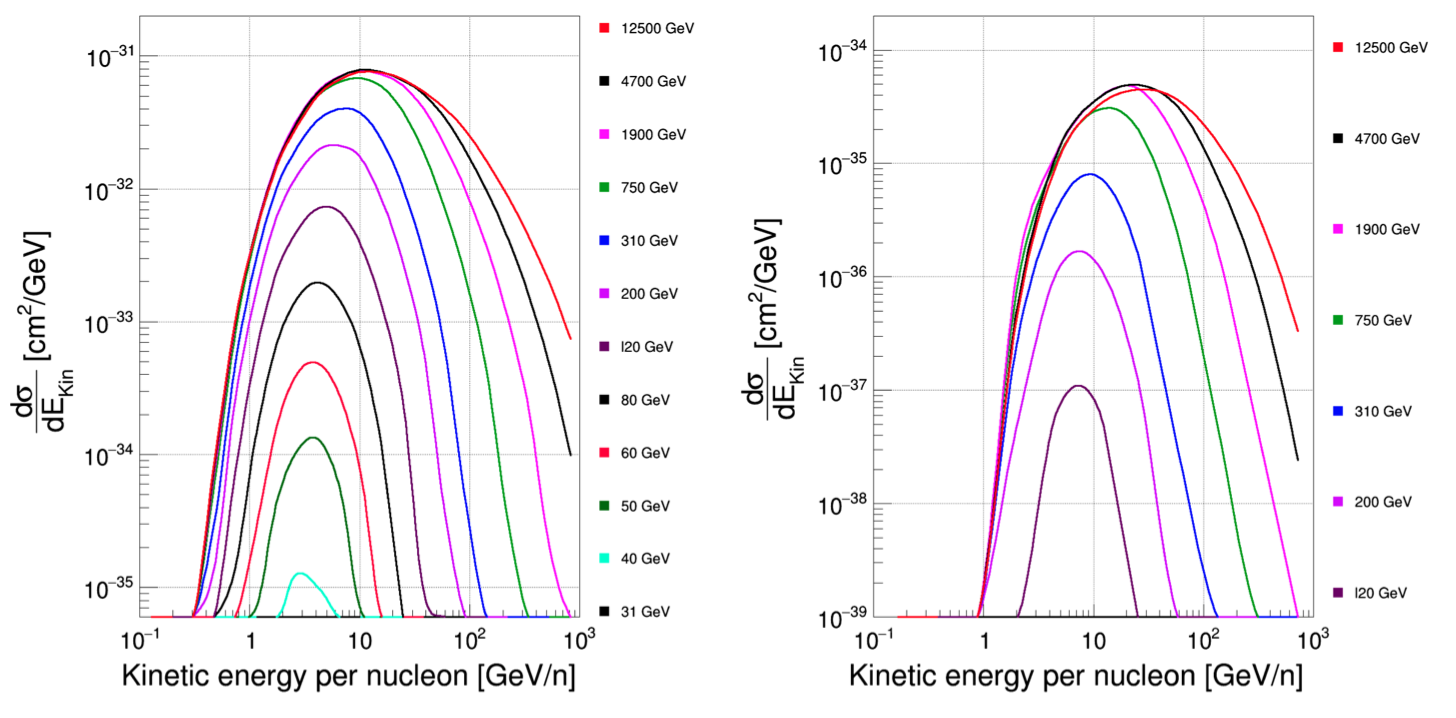
\includegraphics[width=\textwidth]{figures/production_xs_shukla.png}
    \caption{Production cross section for antideuterons (left) and \ahe\ (right), as a function of the energy of the antinucleus produced, for a range of different projectile energies, taken from Shukla et. al. The \ahe\ cross section includes the effect of antitritons which are produced and subsequently decay to \ahe\ . }
    \label{fig:CR_production_XS}
\end{figure}

The cross sections shown are constrained by data from a variety of accelerator experiments. The list of experiments used to constrain the production cross for antideuterons is shown in figure \ref{fig:dbar_prod_v_rapidity}, while for \ahe\ the data is very scarce for p-p collisions at low energies. In order to validate the production, the authors instead used their model to simulate pp collisions at $\sqrt{s}=7$ TeV, in order to compare with ALICE data. The resulting fit is shown in figure \ref{fig:prod_v_ALICE}, where the uncertainties are obtained by varying the coalescence momentum by 30\%. It can be seen from figure \ref{fig:dbar_prod_v_rapidity}, for $\sqrt{s} \gtrapprox 25$ GeV, there are only measurements at mid-rapidity. However, due to the highly boosted nature of the frame in CR collisions, antinuclei are likely to be produced at very forward rapidities. Thus, further experimental searches at forward rapidity are needed in order to better constrain antinuclei production in high energy CR collisions.  

\begin{figure}
    \centering
    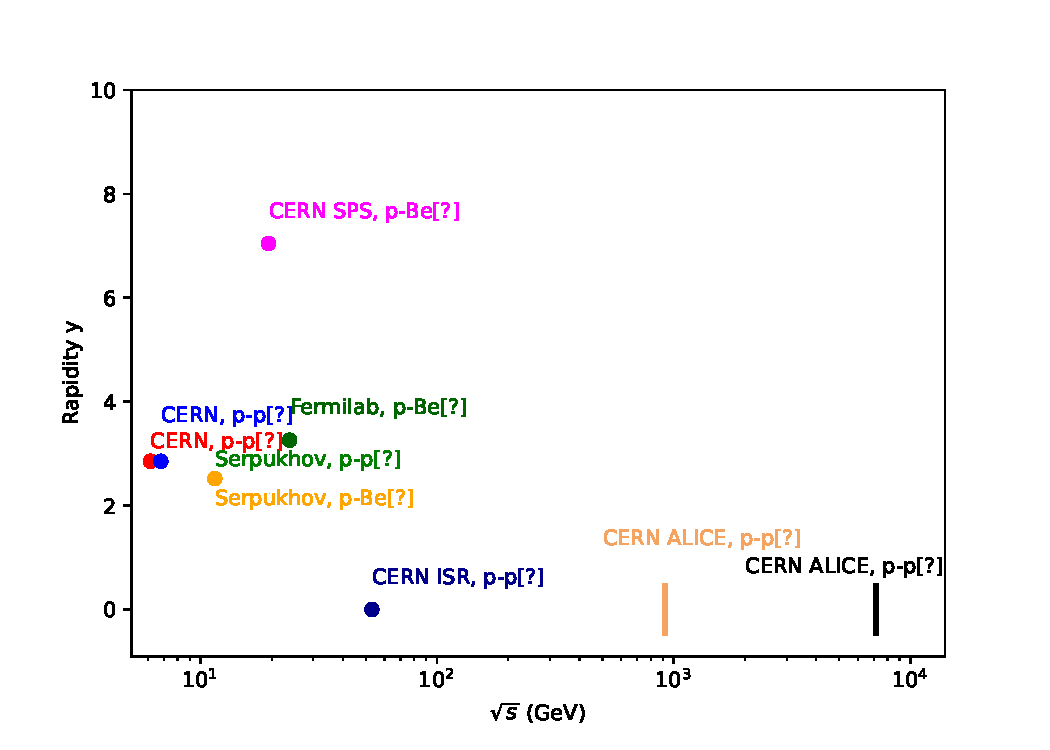
\includegraphics[width=\textwidth]{figures/dbar_production_experiments_sqrts_v_rapidity.pdf}
    \caption{A list of experiments with measurements of (anti)deuteron production, as a function of rapidity and $\sqrt{s}$. The compilation is taken from table 2 in \cite{Gomez_Coral_2018}, based on data in \cite{Diego24, Diego28, Diego31, Diego34, Diego50, Diego51, Diego52, Diego53, Diego54, Diego55, Diego56}.}
    \label{fig:dbar_prod_v_rapidity}
\end{figure}

\begin{figure}
    \centering
    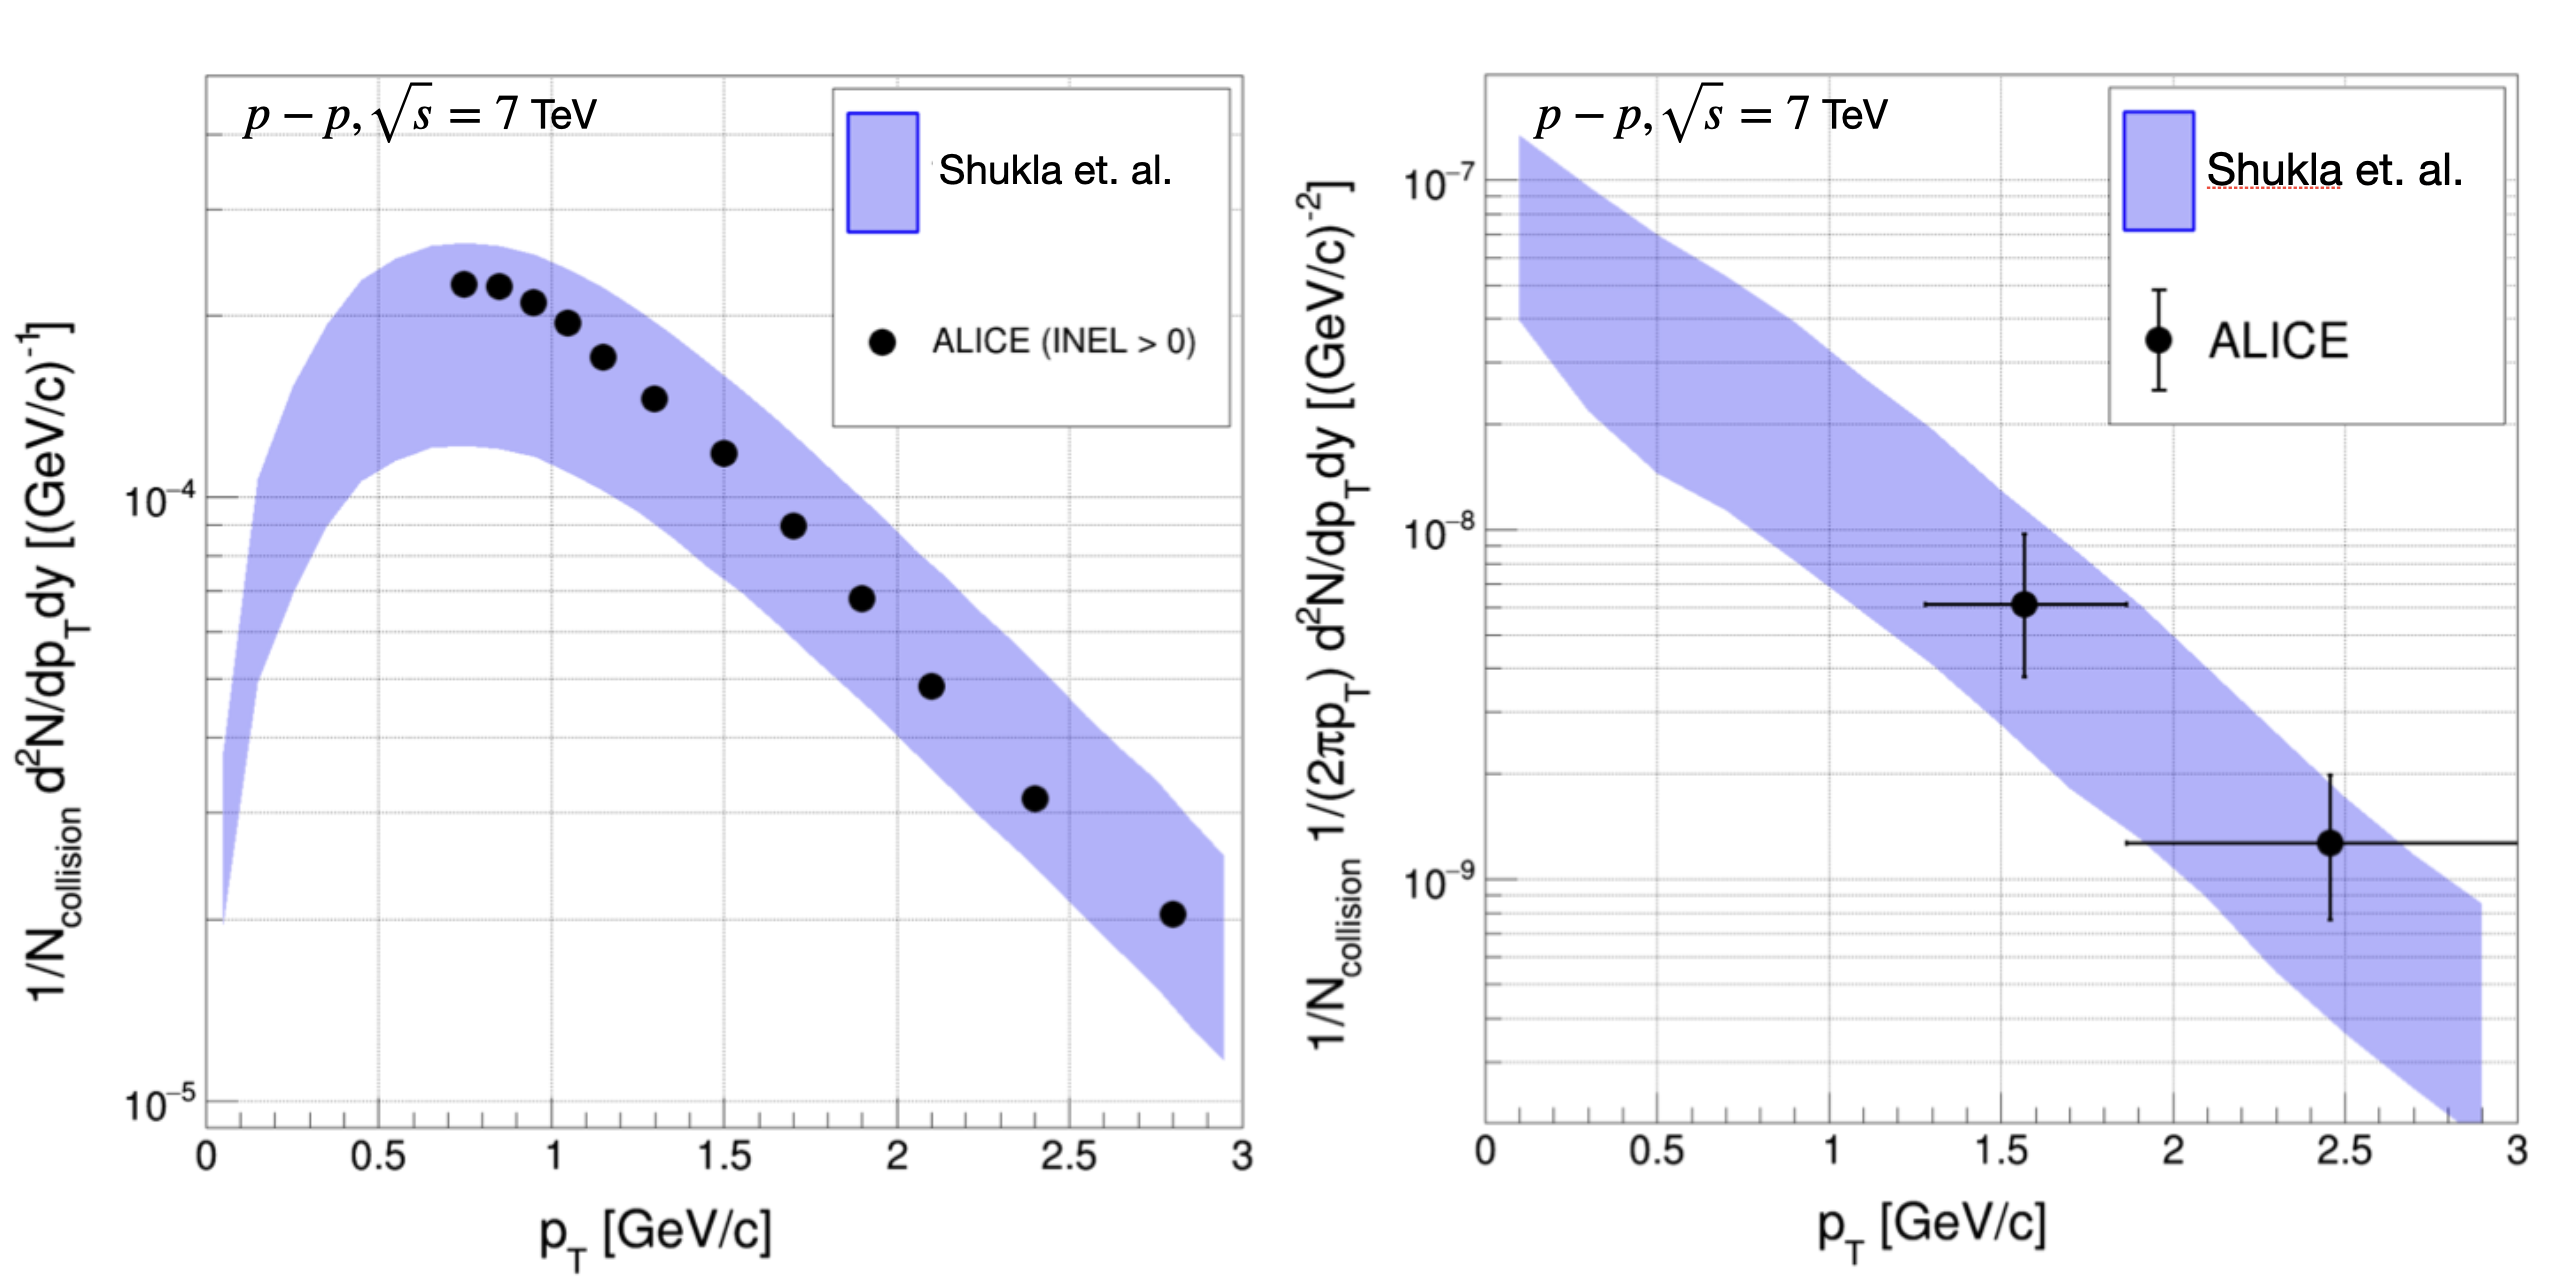
\includegraphics[width=\textwidth]{figures/production_xs_ALICE_comparison.png}
    \caption{Comparison of the antideuteron (left) and \ahe\ (right) spectra obtained by Shukla et. al. with ALICE data for $\sqrt{s}=7$ TeV pp collisions.}
    \label{fig:prod_v_ALICE}
\end{figure}

Once these cross sections are obtained, they need to be folded with the galactic cosmic ray spectrum at each point in space. This spectrum spans over more than 11 orders of magnitude if all particles are considered, and at least 6 orders of magnitude for protons. A compilation of available data on the cosmic ray spectrum can be found in figure \ref{fig:CR_spectra_Thomas}. The implementation of this process in Galprop is done by implementing the cross section above, and thus calculating equation \ref{eq:secSourceTerm} at each point in the space/momentum grid employed in GALPROP. For a more detailed discussion of Galprop see section \ref{sec:GALPROP}. Also shown in the left of this figure is the source term of antideuterons, as a function of both the incoming particle momentum and the momentum of the produced antideuteron. From this it can be seen that the most important momentum range to probe is 100-500 GeV/$c$. 

\begin{figure}
    \centering
    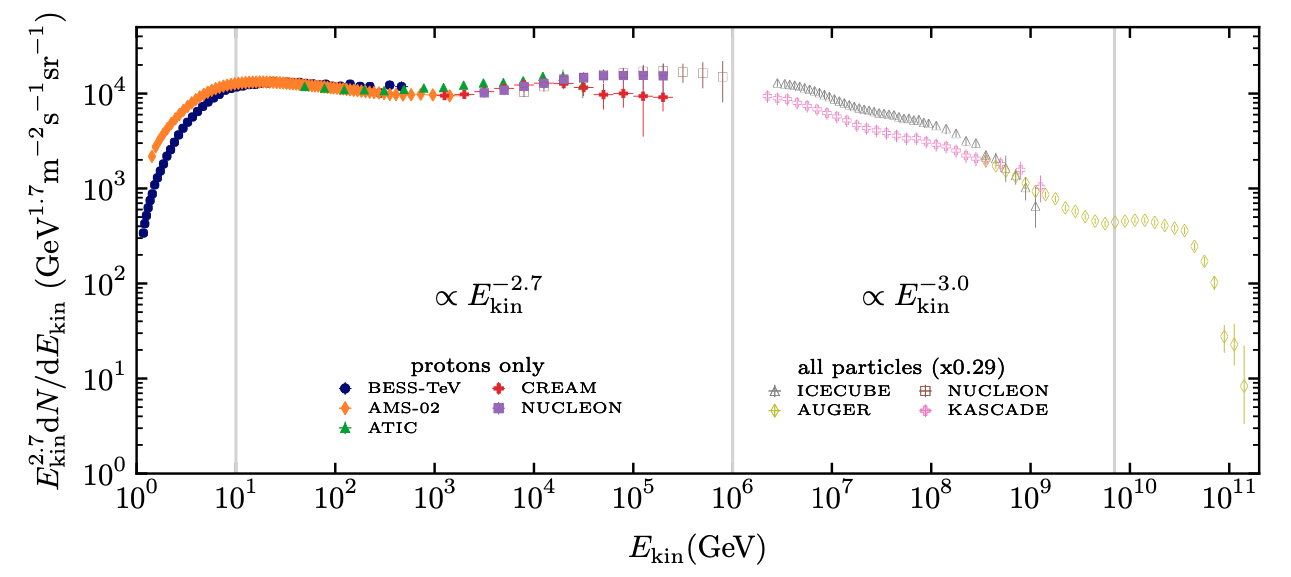
\includegraphics[width=\textwidth]{figures/ThomasP_cosmic_ray_spectra.png}

    \caption{Cosmic ray particle spectra, for protons and all particles, from relevant experiments. Figure taken from \cite{ThomasThesis}. }
    \label{fig:CR_spectra_Thomas}
\end{figure}
\begin{figure}
    \centering
    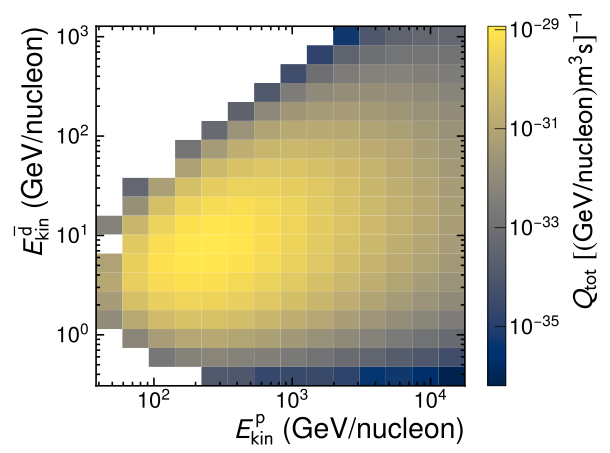
\includegraphics[width=0.75\textwidth]{figures/dbar_2dplot_production.png}
    \caption{The source term of antideuteron from high energy cosmic ray collisions, as a function of the incoming proton energy and the outgoing antideuteron energy. The figure is taken from \cite{Serksnyte:2022onw}.}
    \label{fig:dbar_2d_source_CR}
\end{figure}




\subsubsection{Weakly interacting massive particles (WIMPs) dark matter}\label{sec:WIMPS}

\begin{figure}
    \centering
    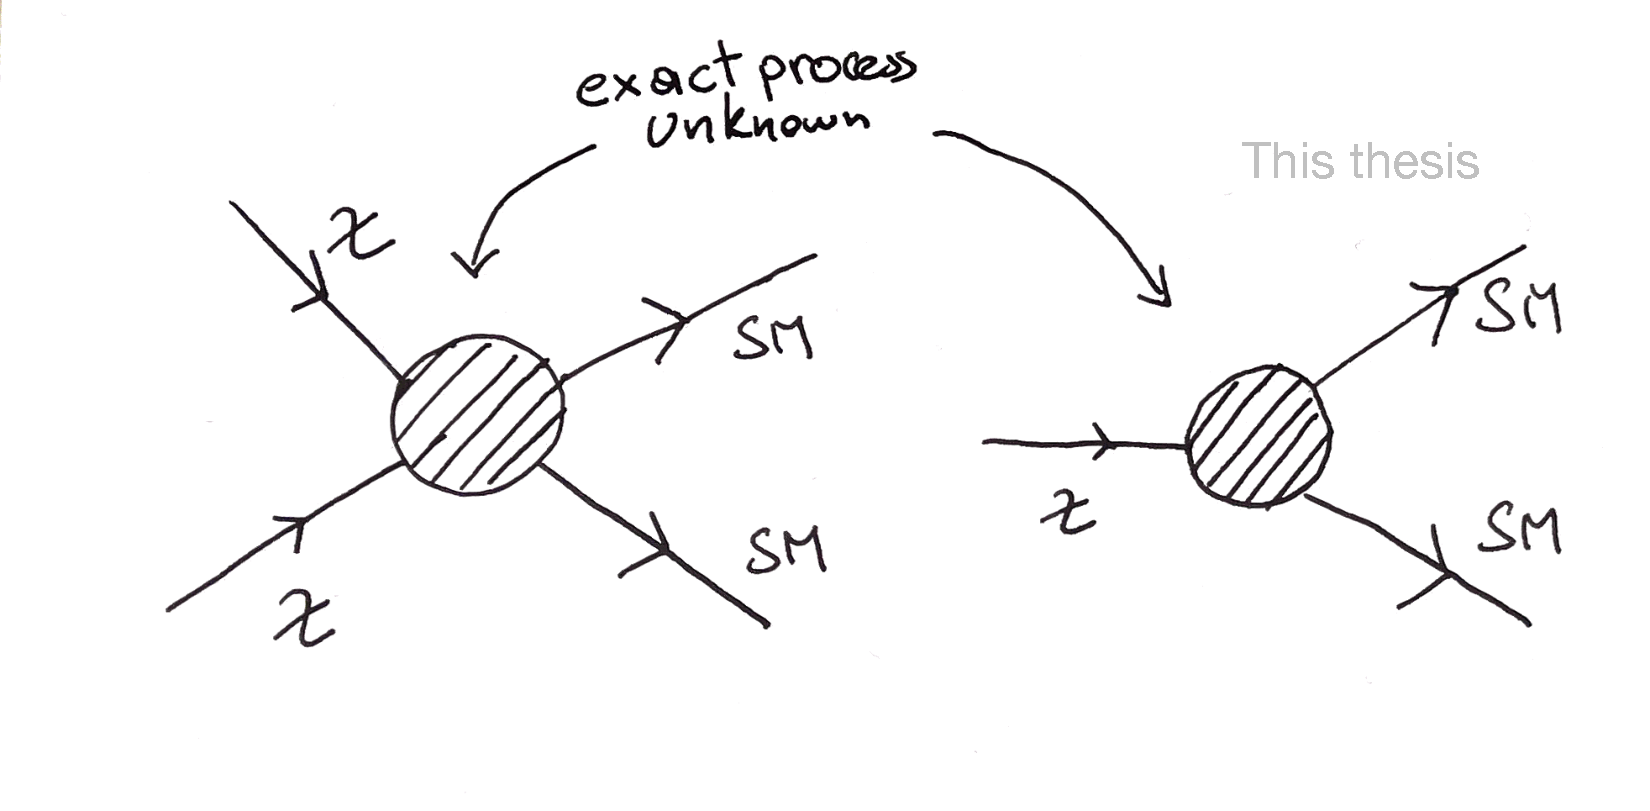
\includegraphics[width=\textwidth]{figures/DM_processes.pdf}
    \caption{A schematic of dark matter pair annihilation into standard model particles (left) and of dark matter decay into standard model particles (right) for a WIMP particle. The exact process by which this would occur is not known, and therefore currently model dependent. Note that a scattering process between a dark matter and a standard model particle would look very similar to the diagram on the left, with the space and time axes inverted (i.e. change the arrow direction of the top dark matter and bottom standard model particle). However, this scattering might happen via a very different internal process, so the two cannot be directly related in a model independent way.}
    \label{fig:DM_ann_decay_processes}
\end{figure}
Some WIMP dark matter theories predict that WIMP annihilations can produce a significant amount of antinuclei \cite{Ibarra:2012cc, Korsmeier:2017xzj, cookbook}. Such theories are based on the assumption that dark matter is made of particles (hereinafter denoted $\chi$), which during the big bang were in thermal equilibrium with SM particles. This requires that some SM processes were able to create $\chi$. This can be understood kinematically from the available energy in such a process. If the SM particles colliding would have an energy which exceeds \Vs\ = $2\mathrm{m}_\chi$, they could create a dark matter particle pair. Similarly, the dark matter particles would have to be able to either decay or annihilate into SM particles, in order to maintain the equilibrium, as shown in figure \ref{fig:DM_ann_decay_processes}. We shall first consider the scenario that the dominant mechanism of interaction for dark matter into SM particles was decau. If they would only decay, there would have to be some mechanism which reduces this decay rate by many orders of magnitude once the thermal equilibrium is broken and dark matter decoupled from baryonic matter, since otherwise dark matter would have continued to decay rapidly and almost none would be left today\footnote{This would require a mechanism to destabilize dark matter particles in the very hot and dense medium which existed just after the big bang. During the period before dark matter decoupled -- which is assumed to have occurred around the quark-gluon-plasma phase of the early universe, i.e. $10^{-12}$s - $10^{-5}$ s after the big bang -- the decay rate would have had to be much less than $10^{-5}$s in order to achieve thermal equilibrium. In order to remain stable after decoupling, its lifetime would have to exceed the current lifetime of the universe, around $10^{17}$s. In medium modifications of decay widths is a known effect \cite{Riek_2010}, however, it is difficult to imagine a process which modifies the lifetime of such particles by at least 20 orders of magnitude.}. For dark matter annihilations no such effect is necessary, since the annihilation rate naturally decreases with the dark matter density squared (this will be explained in equation \ref{eq:DM_source_term}). Thus, as the universe expands, dark matter with a coupling into baryons through annihilation will naturally freeze out and its abundance from this point would remain almost constant. However, given that residual annihilations are still possible when two dark matter particles meet, any SM particles produced could be observed and shine a hint on its nature. It is this exact process which is looked for in cosmic ray antinuclei signals. A cold dark matter particle pair annihilating at rest has \Vs\ = $2\mathrm{m}_\chi$. The net baryon number would be 0 in such a process, resulting in no further penalty for the production of multiple antinucleons. Per definition, WIMPs interact only weakly, and thus their initial annihilation would occur through a weak channel. Since the weak bosons couple to all other standard model particles, this enables the production of particles such as antinuclei. \\
%(such as W$^+$W$^-$ or b$\overline{\mathrm{b}}$)



The spectrum and yield of antinuclei produced in these annihilations has to be estimated based on known standard model processes. To this end, Monte Carlo event generators are employed \cite{Ibarra:2012cc, Coogan_2017, cookbook}, in which the initial state is the first state of standard model particles which is assumed to occur in the annihilation process, with a COM energy equal to twice the dark matter mass \dmm \cite{cookbook}.%particle physics cookbook, also https://arxiv.org/pdf/hep-ph/9904481.pdf}. 
The exact initial state of SM particles is not known, but commonly the channels \WW\ and \bb\ are considered \cite{Coogan_2017, Ibarra:2012cc}. These two form a convenient subset, as over the range of expected masses (~10 GeV to about 1 TeV), they are consistently two of the more optimistic scenarios, and cover the different parameter space within these optimistic scenarios \cite{cookbook}. This can be seen from figure \ref{fig:DMsource_spectra_other_channels}. 
Since event generators do not produce (anti)nuclei -- but only the individual nucleons -- the (anti)nuclei yields and spectra have to be calculated using the coalescence model. One particular annihilation channel has recently been proposed \cite{Winkler_2021}, which suggests a boost of the \ahe\ yield through an intermediate decay to $\overline{\Lambda}_{\overline{\mathrm{b}}}$.
While the branching ratio for the process $\overline{\Lambda}_b \rightarrow $ \ahe\ $+X$ is not well constrained by data, the default tunes\footnote{Tunes when used to talk to event generators are the specific settings which are used for the event generator to more accurately reproduce a given result, e.g. the proton spectra at a given energy.} of the event generators tends to underestimate this, and thus the amount of \ahe\ production (it also has an impact on the antideuteron production, but far less, as can be seen in section \ref{fig:Results_dbar_fluxes_diff_DM_masses} below). In particular, a discrepancy is observed between two commonly used event generators (Pythia \cite{pythia} and EPOS \cite{EPOS}) of about a factor 3. In order to rectify this, a special setting of the Pythia event generator is used to reproduce the branching fraction close to the one of EPOS. This setting is referred to as the $\overline{\Lambda}_b$ tune in the following discussion. According to these results, there is an almost 10 fold increase in the resulting detectable \ahe\ flux, in particular at high energies around 10 GeV/A. This is of particular interest since according to the authors, such an increase would cause a signal detectable by the AMS-02 experiment, with an event rate of about 1/year.  The authors also consider the decay of $\overline{\Lambda}_b$ through light intermediator particles, which provides a slightly different spectrum.\\
So in addition to the spectra obtained using default event generators from \cite{Coogan_2017, Ibarra:2012cc}, the spectra incorporating the $\overline{\Lambda}_b$ decay are also considered as part of this thesis. All the relevant spectra from these processes for antideuterons and \ahe\ are shown in figure \ref{fig:DMsource_spectra}. \\ 
\begin{figure}
    \centering
    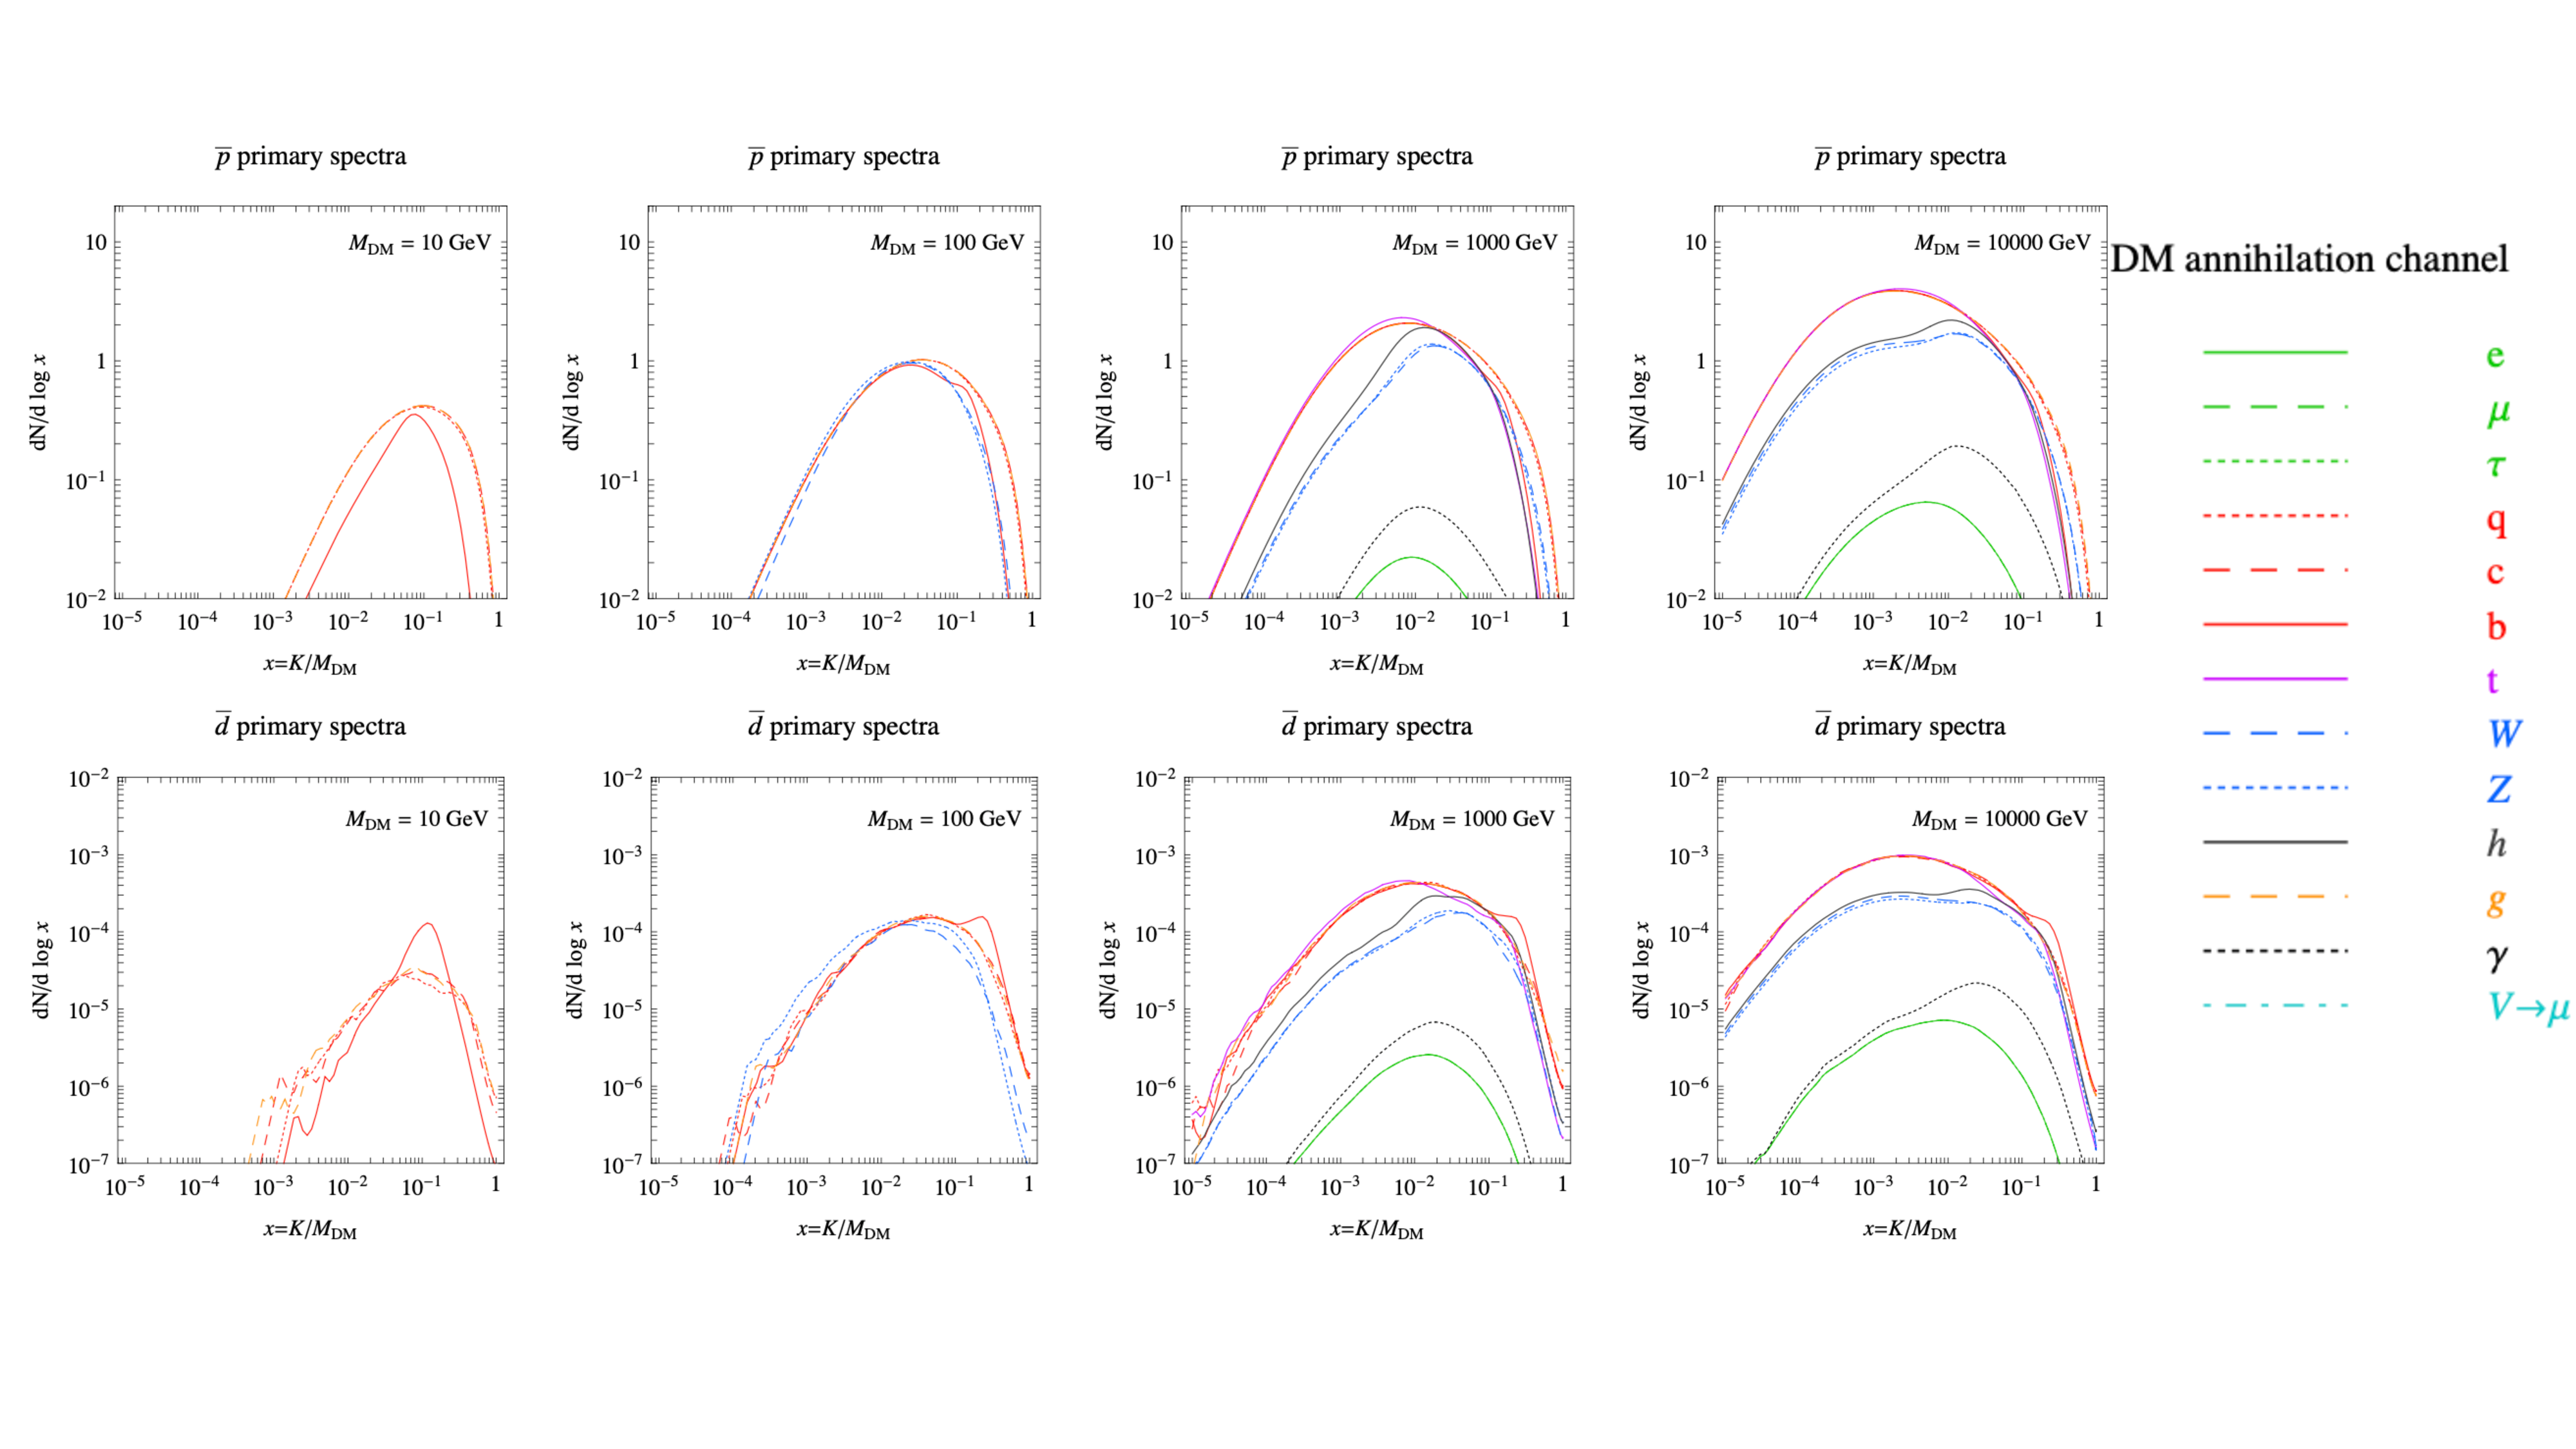
\includegraphics[width=\textwidth]{figures/cookbook_other_channels.pdf}
		\caption{Antiproton (top) and antideuteron (bottom) spectra from dark matter annihilations as a function of the antinuclei kinetic energy per nucleon, normalized to a single annihilation event, for a wide variety of initial SM states. This figure is taken from \cite{cookbook}.}
    \label{fig:DMsource_spectra_other_channels}
\end{figure}
\begin{figure}
    \centering
    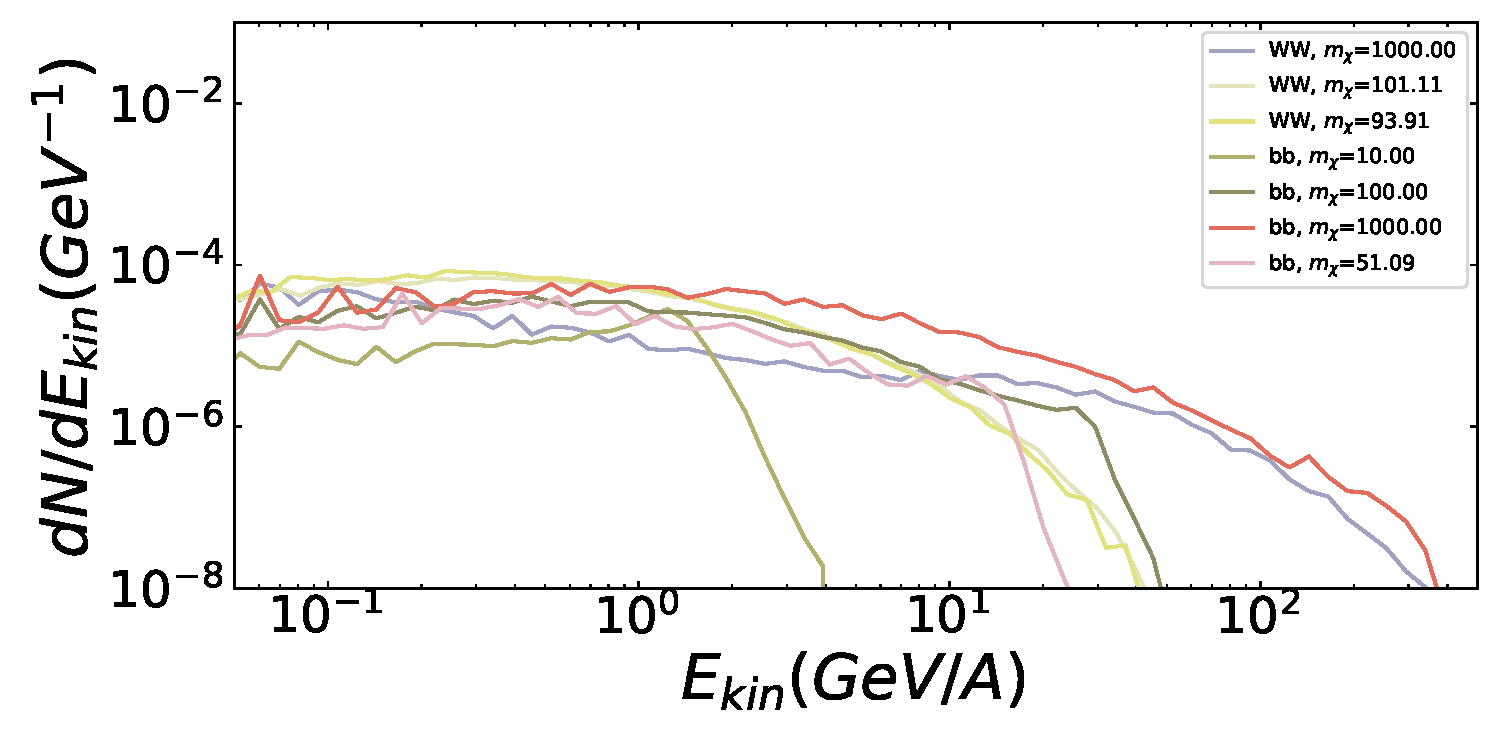
\includegraphics[width=0.45\textwidth]{figures/dbar_injectionSpectra.pdf}
    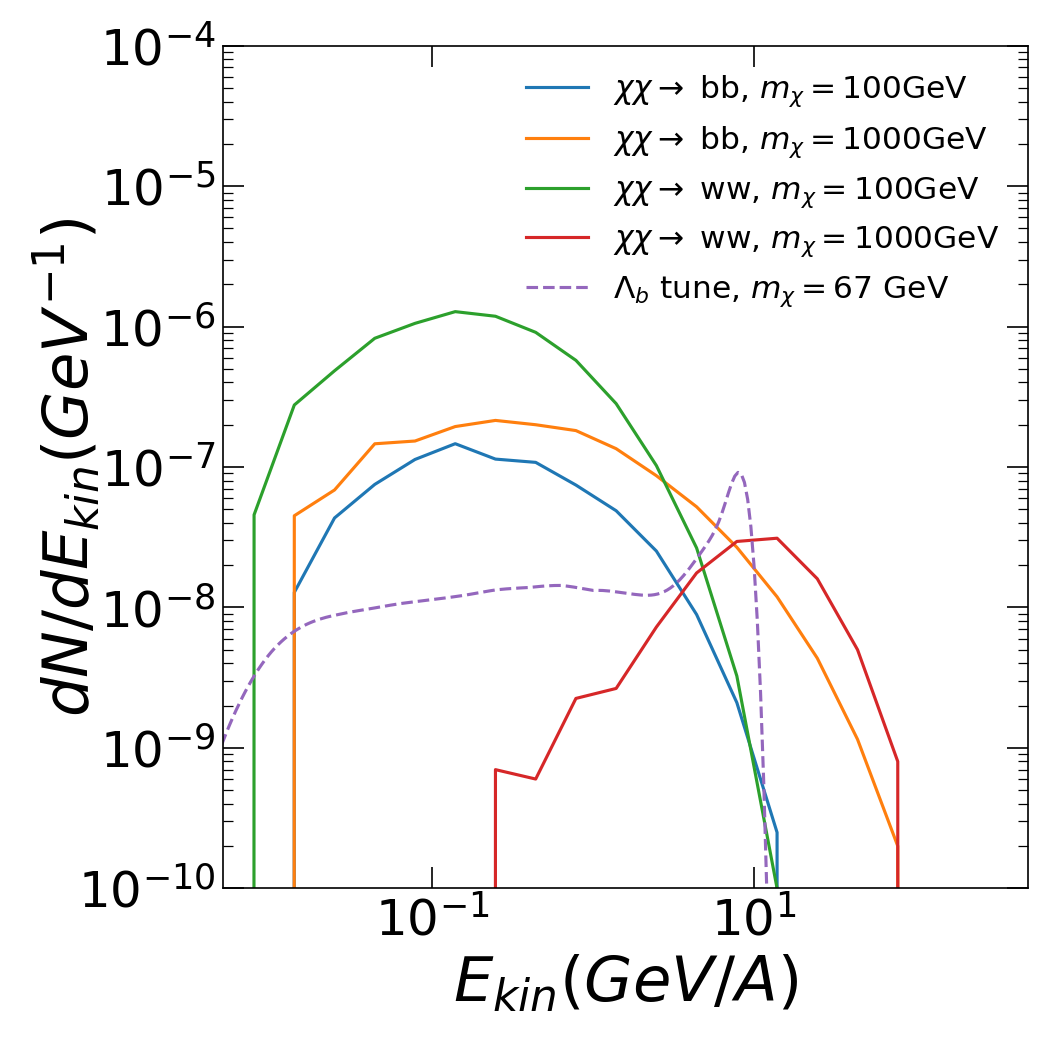
\includegraphics[width=0.45\textwidth]{figures/He3bar_injection_channels.png}
    \caption{Antideuteron (left) and \ahe\ (right) spectra from dark matter annihilations as a function of the antinuclei kinetic energy per nucleon, normalized to a single annihilation event. Spectra for \WW\ and \bb\ channels are taken from \cite{Ibarra:2012cc}, $\overline{\Lambda}_b$ tune is taken from \cite{Winkler_2021}.}
    \label{fig:DMsource_spectra}
\end{figure}


Since decoupling from baryonic matter, the dark matter would have cooled with the expanding universe, and thus is assumed to be at a similar temperature as the cosmic microwave background (CMB) today, of about 2.7K \cite{CMB_temp}. This is referred to as cold dark matter. Another consideration which supports cold dark matter is that the majority seems to be gravitationally bound within galaxies and galaxy clusters \cite{Doetinchem_2020_review, GAPS_setup_Bird, Baushev_2013, DM_review}. As such, the COM frame is assumed to be the same as the galactic frame, and no boost from the initial velocities are necessary. This is convenient, since one can therefore simply take the spectrum of produced antinuclei per dark matter annihilation -- which is obtained from applying a coalescence afterburner to the output of a Monte Carlo event generator -- and multiply it by the local annihilation rate of dark matter. Thus, one can write the source term $q(\vec{r}, E)$ for WIMP dark matter as

\begin{equation}\label{eq:DM_source_term}
    q(\vec{r}, E) = \frac{1}{2} \left( \frac{\rho_{\chi}(\vec{r})}{m_\chi}\right)^2 <\sigma v > (1+\epsilon) \frac{dN}{dE},
\end{equation}
where the factor $1/2$ comes from symmetry considerations for majorana dark matter\footnote{See section \ref{sec:IntroMajoranaDiracDM} for a discussion on the difference between Majorana and Dirac dark matter.}, the term $\left( \frac{\rho_{\chi}(\vec{r})}{m_\chi}\right)^2$ is the square of the number density of the WIMP dark matter, which is then multiplied by the velocity averaged dark matter annihilation cross section $<\sigma v>$, giving the rate of dark matter annihilations for a given point in space. The term 1+$\epsilon$ accounts for contributions from other particles which are produced and subsequently decay into the antinucleus in question, at timescales longer than the consideration of the MC event generator. The value of $\epsilon$ is 0 for antideuterons and 1 for for \ahe, to account for \atrit\ . The final term of equation \ref{eq:DM_source_term} is the spectrum of produced antinuclei normalised to a single dark matter annihilation. The terms of equation \ref{eq:DM_source_term}, their contraints and degeneracies are discussed below.\\

The dark matter density profile $\rho_\chi(\vec{r})$ affects both the total amount of antinuclei produced as well as their initial distribution. This parameter can be constrained from measurements of the Milky Way's rotation curve, similarly to how it is done for other galaxies. However, measuring the rotation curve of the Milky Way involves extra challenges, given that we are measuring from within. This is due to the fact that for other galaxies, measuring the difference in velocity through red/bluehisft at different positions is sufficient to measure the rotation curve, whereas for our own galaxies we need the measure both the 3d position and velocity of many stars. The most promising technique to do this is Very-Long-Baseline-Interferometry, which essentially uses telescope arrays spanning multiple continents as interferometers \cite{Charlot_2020}. A more detailed discussion of measuring rotation curves can be found in \cite{Sofue_2016, Sofue2020}. Our galaxy's rotation curve  has been reported in \cite{Sofue2020}, found by combining multiple existing measurements. It is reproduced in figure \ref{fig:MilkyWayRotationCurve}. \\

\begin{figure}
    \centering
    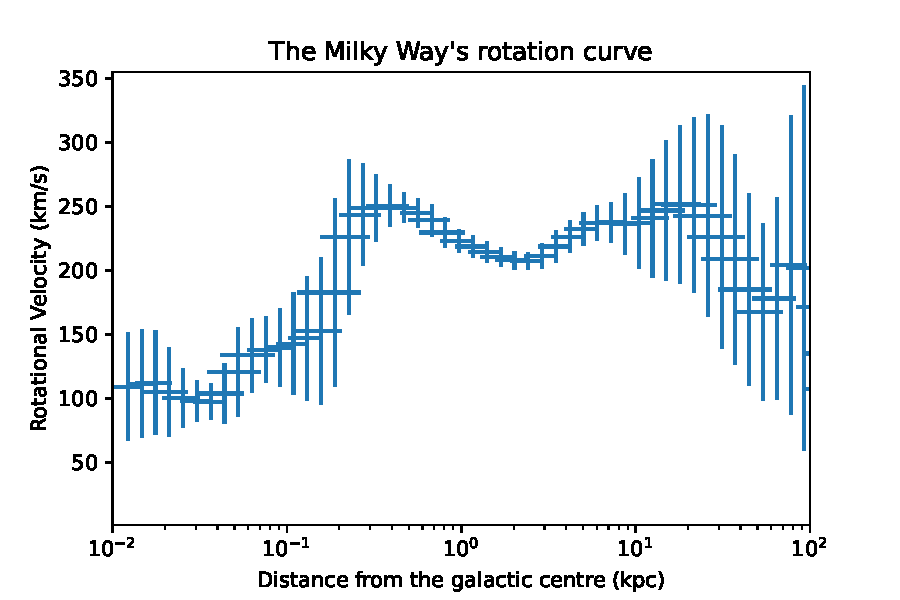
\includegraphics[width=\textwidth]{figures/RotationCurveMilkyWay.pdf}
    \caption{Rotation curve of stars in the Milky Way, as a function of distance from the galactic center. Reproduction of data reported in \cite{Sofue2020}.}
    \label{fig:MilkyWayRotationCurve}
\end{figure}

In order to fit such rotation curves, our galaxy is conventionally split into individual parts, each of which can be assumed to have a simpler shape. The usual breakdown of these parts is shown in table 3, and further details can be found in \cite{Sofue_2016}. The gravitational potentials of these parts can then be summed up linearly, and the rotational velocities caused by each such potential can be added in quadrature. In order to fit the contribution from dark matter, the shape of the dark matter distribution has to be chosen a priori, such that the exact parameters and normalization can then be obtained from the fit. This is an important point, since the total normalization of the dark matter profile is not well constrained. Rather, the relatively well constrained rotation curve in the proximity of the solar system results in the fact that the local dark matter density $\rho_\chi(\vec{r}=r_\odot) := \rho_\chi^\odot$ is much better constrained than the total normalization of the dark matter profile. Thus, the different dark matter profiles are constrained to their value at $r_\odot = 8.5$kpc\footnote{The value is currently estimated to be 0.4GeVcm$^-3$ \cite{DM_review, Ibarra:2012cc, Sofue_2016, Sofue2020, PDG2022}.}, the estimated position of our sun. \\
\begin{table}[h]
    \centering
    \begin{tabular}{|c|c|c|c|}
        \hline
        Part & Shape & Extent & Total Mass \\
        \hline
        Central black hole & Point mass & $<$ 0.1pc & 3.6$\times$ 10$^6$ M$\odot$ \\
        \hline
        Buldge(s) & Spherical exponential & $<$1kpc & 10$^{11}$ M$\odot$ \\
        \hline
        Flat disk & Constant flat disk & $<15$kpc & $\approx$10$^{10}$ M$\odot$ \\
        \hline
        Dark matter halo & vaires & 100s of kpc & 10$^{12}$ M$\odot$ \\
        \hline
    \end{tabular}
    \label{tab:MilkyWayBreakdown}
    \caption{Individual axissymmetric parts of the Mikly Way used for fitting rotation curves. The distinction is made in order to simplify the fit, rather than a hard distinction within the actual galaxy. Non-axissymmetric components are neglected for rotation curves, based on the assumption that any effects would cancel out when averaged over the full rotation. The values for the total mass were taken from \cite{Sofue_2016}. The extent column is approximate and given in order to help the reader visualise the distributions. Due to the distributions being exponential, they only asymptotically approach 0.}

\end{table}

There are several profiles on the market, which achieve similar goodness-of-fit when fit to account for the dark matter component in the rotation curve \cite{Ibarra:2012cc}, while also achieving the required normalisation at $r_\odot$. The ones used in this work are the Navarro-Frenk-White(NFW) profile \cite{Navarro_1996}, shown in equation \ref{eq:NFW}

\begin{equation}\label{eq:NFW}
    \rho_\chi^{NFW}(\vec{r}) = \frac{\rho_0}{(r/r_s)[1+(r/r_s)]^2},
\end{equation}
with scale radius $r_s=$24.42kpc, the Einasto profile \cite{Einasto}, shown in equation \ref{eq:Einasto}

\begin{equation}\label{eq:Einasto}
    \rho_\chi^{Einasto}(\vec{r}) = \rho_0 \mathrm{exp} \left\{ -\frac{2}{\alpha}\left[ \left( \frac{r}{r_s}^\alpha -1\right) \right] \right\},
\end{equation}
with $\alpha$=0.17 and $r_s$=28.44kpc, and the much shallower isothermal profile \cite{isothermal} and the isothermal profile, shown in equation \ref{eq:isothermal}
\begin{equation}\label{eq:isothermal}
    \rho_\chi^{isothermal}(\vec{r}) = \frac{\rho_0}{r^2+r_s^2},
\end{equation}
with $r_s$=4.38kpc. The profiles are plotted in figure \ref{fig:DMProfiles}, using best fit values taken from \cite{Ibarra:2012cc}. It can be seen that the isothermal profile has a very shallow rise towards the galactic center, while the Einasto profile rises very steeply. The NFW profile lies between the two\footnote{At very small radii, the NFW profile becomes larger than the Einasto profile.}, and is often used preferentially \cite{Korsmeier:2017xzj, Ibarra:2012cc, Coogan_2017}. The stark difference between them is due to their origin. The isothermal profile is motivated purely by the fit to galactic rotation curves, while the NFW and Einasto profiles are motivated by the addition of numerical N-body simulations, which the isothermal profile struggles to replicate \cite{Lin_2019}. All these profiles assume spherical symmetry. Numerical simulations seem to prefer a triaxial ellipsoid, however, given the lack of data for the tidal motion of stars in the Milky Way, it is currently not possible to narrow down the shape more exactly than a simple spherically symmetric model. These three profiles cover most of the available parameter space for the dark matter profile. \\

\begin{figure}
    \centering
    \includegraphics[width=0.8\textwidth]{figures/DMProfiles_distributions_log.png}
    \caption{Dark matter density profiles used in this work, as a function of the distance to the galactic centre. The best fit values for each profile are taken from \cite{Ibarra:2012cc}.}
    \label{fig:DMProfiles}
\end{figure}

It is important to ask why the stark differences towards the center of the galaxy play such a reduced role that all three of these profiles are able to fit the data, and if such differences would therefore make any interpretation of an antinuclei flux from dark matter impossible. The answer to the first part of the question is twofold. Firstly, it is very challenging to measure the rotation curve of our own galaxy with high precision at positions far from the solar system, as can be seen from the uncertainties in figure \ref{fig:MilkyWayRotationCurve}. Secondly, the gravitational effect of the dark matter halo contributes mainly at distances larger than $\approx$ 2 kpc from the galactic center, where the presence of extra mass at the centre of our galaxy (from a steeper profile) is not as strongly felt. This can be seen from figure \ref{fig:RotationCurveFit}. The second question also has a fortunate answer: the effect of different profiles on a potential local flux of antinuclei from a dark matter source is rather small, as is discussed in section \ref{sec:ResDMProfiles}. 

\begin{figure}
    \centering
    \includegraphics[width=\textwidth]{figures/Felix_rot_curve_fit.png}
    \caption{Fit of the rotation curve of the Milky Way, with a NFW profile. Figure is taken from \cite{FelixThesis}, based on work in \cite{Baushev_2013}.}
    \label{fig:RotationCurveFit}
\end{figure}
To summarize: the dark matter density profile in our galaxy is constrained by measurements of the Milky Way's rotation curve. Measuring the rotation curve is a non-trivial process, which involves measuring the 3d position of stars within our own galaxy. The most modern method to achieve this is Very-Long-Baseline-Interferometry (VLBI), which uses telescope arrays spanning continents as a giant interferometer. Once the rotation curve is measured, the effect from luminous matter is accounted for, and the remainder is assigned to the dark matter component. Due to the experimental uncertainties involved in measuring the velocity of far away objects, this leaves a significant plausible parameter space for the shape of the dark matter profile towards the center of our galaxy. \\

The second term of equation \ref{eq:DM_source_term} is the dark matter mass, \dmm\ . The dark matter mass is a free parameter, with possible values ranging from very light dark matter\footnote{A popular light dark matter model is the axion model \cite{axion_review}.} below the eV range all the way to the WIMP dark matter discussed in this work, with plausible mass ranges from 10s of GeV to the TeV range. As discussed in section \ref{sec:IntroWIMPs}, the appeal of WIMP dark matter is that the expected weak cross section of such a particle in the very early universe would yield a population today of the same magnitude as we observe (a mathematical derivation can be found in \cite{DM_review} and is reproduced in section \ref{sec:IntroWIMPs}). It would also explain the lack of evidence for the production of dark matter at accelerators, since we might at this point not yet have reached the energies required to produce such particles. Finally, many extensions of the standard model naturally include such a particle, most notably super symmetry, which requires the neutralino, a particle which would fit the WIMP description \cite{Supersymmetry_primer}. This was a rather enticing argument at the inception of WIMPs in the 80s, however, by now the parameter space for supersymmetric theories has become very small \cite{Supersymmetry_primer}, due to null observations at accelerators including the LHC. This has made the question of how to incorporate such a particle into the Standard Model more difficult, and thus increased the interest in alternative dark matter candidates, which are discussed in section \ref{IntroOtherDM}.           



Since the exact nature of dark matter remains a mystery, a priori a wide range of masses is possible. However, direct detection experiments have placed limits on the dark matter-matter interaction cross sections, as a function of the dark matter mass \cite{XENON2, Lux} and a recent compilation of these limits is shown in figure \ref{fig:DirectDetectionLimits}. It is not possible to relate this interaction cross section with the dark matter self annihilation cross section $<\sigma_{ann} v>$ on general grounds, since they might depend on very different couplings. But it can help us make an informed decision on WIMP masses. As can be seen from figure \ref{fig:DirectDetectionLimits}, for masses over a few 10s of GeV, constraints become very strong, limiting the cross section to below a billionth of a pb. Upcoming next generation experiments, such as XENONnT \cite{XENON_new_physics} and Darkside20k \cite{Aalseth_2018}, are expected to push these limits within reach of the neutrino coherent scattering background. If these experiments also do not see a signal, it would eliminate the possibility of background free detection using direct detection methods. 

\begin{figure}
    \centering
    \includegraphics[width=\textwidth]{figures/Direct_detection_limits.png}
    \caption{Limits from direct detection experiments on the dark matter - nucleon interaction cross section, as a function of the dark matter mass. The figure is taken from \cite{Zyla_direct_detection}.}
    \label{fig:DirectDetectionLimits}
\end{figure}

The chosen mass has a direct effect on all three remaining terms of equation \ref{eq:DM_source_term}: i) $\frac{1}{m_\chi^2}$, ii) $\frac{dN_{\mathrm{\bar{p}, \bar{d}, {^3\overline{He}}}}}{dE}$  and iii)$<\sigma v>$. The effect on i) is trivial, and reduces the overall normalization of the antinuclei source term for higher \dmm\ . The mass' effect on ii) is based on the amount of energy available for the production of (anti)nuclei, as well as for their kinetic energy. For higher masses, the antinuclei yields increase non-trivially, but slower then the inverse square reduction from the first term. Additionally, the extra energy available for higher masses translates into a spectrum peaked at higher momenta. This depends not only on the available energy, but also on the decay channel. The $\frac{dN_{\mathrm{\bar{p}, \bar{d}, {^3\overline{He}}}}}{dE}$ spectra used for the antideuteron and \ahe\ results shown in this chapter are shown in figure \ref{fig:DMsource_spectra}. The effect of \dmm\ on $<\sigma v>$ is mostly experimental, since $<\sigma v>$ is constrained from antiproton measurements. 

Any dark matter annihilation process which can result in antideuterons must of course also produce antiprotons. However, contrary to heavier antinuclei, antiprotons are also copiously produced in other processes, due to the much lower energy threshold required for producing a single antinucleon, and the loss of the need to coalesce multiple antinucleons into a single compound antinucleus. This results in a significant and well constrained antiproton flux, which has been measured by the AMS collaboration \cite{AMS_pbar_systematics_discussion, AMS_pbar_interpretation1}. Thus, any model chosen must not produce a dark matter component for antiprotons which is incompatible with those measurements. These limits are expressed in terms of $<\sigma v>$ as a function of \dmm\ . This representation is chosen since $\rho_\chi$ can be measured independently, and $<\sigma v>$ varies much more slowly with \dmm\ than the other terms. The limits -- which have been extracted by several groups \cite{Cholis_19, Cui_2018, Cuoco_2019, Cuoco_2018} and compiled by \cite{Doetinchem_2020_review}-- are shown in figure \ref{fig:DMSigmaVLimits}. Indicated in the figure is the maximum limit on $<\sigma v>$, as well as the thermal relic cross section ($\approx 1pb \times c$)\footnote{See the derivation in section \ref{sec:IntroWIMPs} for more details.}. 

Also indicated in this figure is the area in which a possible excess of antiprotons was observed in the \pbar\ spectrum measured by the AMS collaboration, which could hint at a dark matter particle within this mass range of 50-100GeV/$c^2$. The different areas correspond to analysis of the same AMS-02 data by different groups, using either a frequentist or a Bayesian approach \cite{Doetinchem_2020_review}. It can be seen from the left hand side of the figure that for low dark matter masses, the limits lie significantly below the thermal value for this cross section. Thus, \dmm\ affects the constraints on  $<\sigma v>$, particularly for low masses. It is also worth noting that these limits have to be extracted for a given dark matter density profile, and thus when exploring the maximum allowed antinuclei flux given the antiproton constraints, the choice of $\rho_\chi(\vec{r})$ is degenerate with the limits on $<\sigma v>$ set by the AMS antiproton limits.\\

\begin{figure}
    \centering
    \includegraphics[width=0.8\textwidth]{figures/PbarLimitsAMS.png}
    \caption{Limits on  $<\sigma v>$ based on AMS antiproton data. Figure is taken from \cite{Doetinchem_2020_review}.}
    \label{fig:DMSigmaVLimits}
\end{figure}

To summarise: WIMP dark matter models predict that dark matter can annihilate and produce antinuclei. The resulting antinuclei source term depends on 4 things: i) the dark matter density profile, ii) the dark matter mass, iii) the dark matter self-annihilation cross section and iv) the produced spectrum of antinuclei, normalised to a single dark matter decay. i) is constrained by looking at the rotation curve of our galaxy, ii) is a free parameter, iii) is constrained from above by antiproton measurements as a function of \dmm\ and iv) is calculated based on coalescence models, which depend on the total available energy and thus \dmm\ . Thus, there are a few notable degeneracies between the different terms of this source function. However, current constraints on these parameters are not stringent and leave open a large, reasonable parameter space which could result in a measureable antinuclei flux from a dark matter source, affirming antinuclei studies as a great tool for the indirect search for dark matter.



\subsubsection{Extragalactic dark matter}
Dark matter is not exclusively bound within galaxies, but is also present in larger cosmological structures, such as galaxy groups \cite{Baushev_2013}. However, the profiles commonly used in order to fit the distribution of dark matter within our galaxy only take into account galactic dark matter, which can be inferred from the fact that such profiles go to 0 at large distances from the galactic centre. This is because to first order, the extragalactic component will vary over length scales bigger than our galaxy, so the gravitational potential caused by the extragalactic dark matter will be roughly constant within our galaxy, thus causing no active force which could be measured. However, such an additional flux of dark matter could indeed annihilate within our galaxy, thus providing an additional source for antinuclei. In this section the difference of this source to the galactic WIMP dark matter source will be qualitatively discussed. Previous work on the topic expects the extragalactic dark matter component to make up about 12\% of the local dark matter abundance close to our solar system \cite{Baushev_2013}. From this, it can be estimated that the extragalactic dark matter is responsible for no more than $\approx 20$\% of the antinuclei flux near earth. \\ 

In order to determine whether the antinuclei flux caused by extragalactic dark matter follows the same assumptions as the galactic component, it is necessary to examine the differences between galactic and extragalactic dark matter. The first difference would be their velocity. Since the galactic component is bound and the extragalactic is not, the extragalactic component's velocity must exceed the escape velocity of the Milky Way, which lies at about 600km/s. This change in velocity may affect 2 terms in equation \ref{eq:DM_source_term}: the self annihilation cross section and the spectrum of produced antinuclei due to the boosted frame in which the collision takes place. \\
Starting with the effect on the self annihilation cross section, the difference might be due to the momentum dependence of the s-wave and p-wave contributions. The s-wave is velocity independent, while the p-wave contribution has a square dependence on the velocity. However, the speeds of 600km/s still only equate to a beta of 0.002, thus the contribution of the s-wave still dominates at these speeds, resulting in no change in regards to galactic dark matter. In a similar fashion it can be shown that the effect of the increased speed on the produced antinuclei spectrum is negligible. \\

The effect which remains is that of the overall normalisation, which is influenced by the extragalactic component to $\rho_\chi$. This extra component would have little to no effect on the rotation curve of our galaxy, and therefore causes a positive offset in comparison to the purely galactic case. The exact nature of this offset should to first order be roughly constant over our galaxy, however, the interaction of the extragalactic dark matter with our galaxy's gravitational pull would cause an increase in the local extragalactic dark matter density in comparison to another point within the local group. Thus, the main difference between the extragalactic dark matter and the galactic dark matter is the consideration of where the majority of annihilations would occur. Finally, we can conclude that since the overall normalisation for antinuclei fluxes from dark matter annihilations is constrained by the maximal allowed flux from antiprotons -- as discussed in section \ref{sec:WIMPS} -- the increase in flux due to an additional extragalactic dark matter component does not significantly impact expectations. \\

\subsubsection{Primordial black holes}\label{Res:PBH}
Another possible source of antinuclei in the cosmos are primordial black holes (PBHs). These objects would have formed very early in the universe, created from overdense regions shortly after the big bang. Their mass is therefore given by the particle horizon at the time of formation, $M_\mathrm{PBH} \approx c^3t/G \approx 10^{15} (t/10^{-23}s)g$ \cite{HAWKING1974, Hawking_PBH}, where $t$ is the time at their formation. These objects can have a large range in different masses, depending on their formation time. Since such low mass black holes would interact only gravitationally, they would meet the criteria for dark matter \cite{Serksnyte:2022onw, Hawking_PBH}. However, as we shall see in this section, they cannot make up the dominant portion of dark matter in the galaxy. \\
Classically, it is impossible for anything - even light - to escape a black hole. However, as shown by \cite{HAWKING1974}, quantum mechanics predicts that black holes will indeed thermally emit (anti)particles, with a characteristic temperature $T = \frac{\hbar c^3}{8\pi GM k_B} \approxeq 1.06 \left( \frac{M}{10^{13}g}\right)^{-1} \mathrm{GeV} k_b^{-1}$ . This process can be understood as particles tunneling out of the black hole, or as virtual antiparticle-particle pairs being created and one partner tunneling through the event horizon into the black hole, preventing recombination. Both methods yield the same results. The lifetime of such black holes scales with their mass as $\tau_\mathrm{PBH} \propto M_\mathrm{PBH}^{-3}$, i.e. they evaporate faster the smaller they are. This results in PBHs emitting many (anti)particles almost simultaneously when they fully evaporate at the end of their lifespan, a process akin to an explosion. The mass of currently evaporating PBHs is in the range of about $\approx 10^{15}g$, since lighter black holes would have already evaporated in the past, while heavier ones will only evaporate in the future. Such PBHs could produce antinuclei during the final stage of their evaporation. \\
The current abundance of PBHs in this mass range is most tightly constrained from $\gamma$-ray searches \cite{FermiLAT_Point_Sources}, to $\frac{\rho_\mathrm{PBH}}{\rho_\mathrm{tot}} < 10^{-26} (M_\mathrm{PBH}/10^{15}g)^{-5/2}$, which means that PBHs cannot make up all the dark matter in our galaxy. These limits include the extragalactic gamma ray background (for masses down to $10^{13}g$) and the galactic gamma ray spectrum (for masses of $\approx 10^{15}g$). Modification of the PBH lifetime due to an extra dimension in string theory could rectify this, allowing PBHs to make up 100\% of dark matter \cite{5d_PBHs}.\\

In this thesis PBHs were considered as a possible source for antideuterons, using a PBH mass of $9.35\times 10^{14}g$. For this mass, PBHs were found from antiproton constraints to make up no more than $f_\mathrm{PBH} = 4\times 10^{-11}$ of all the dark matter in the galaxy. This corresponds to a local rate of PBH explosions of $2\times 10^{-4} pc^{-3}yr^{-1}$. The source term of antideuterons from such events is given by equation \ref{eq:pbh_source_term}

\begin{equation}\label{eq:pbh_source_term}
	q(\vec{r}, p) = \frac{f_\mathrm{PBH} \rho_{\mathrm{CDM}} (\vec{r})}{M_\mathrm{spectrum}}\frac{dN}{dT},
\end{equation}
where $M_\mathrm{spectrum}$ is the typical mass of the PBHs considered, and $\rho_\mathrm{CDM}$ is the cold dark matter density profile, equivalent to the one used for WIMPs. The corresponding antideuteron spectrum per second $\frac{dN}{dT}$ is taken from \cite{Ibarra:2012cc}, and is shown in figure \ref{fig:pbh_source_spectrum}.

\begin{figure}
		\centering
		\includegraphics[width=0.99\textwidth]{figures/pbh_source_spectrum_dbar.pdf}
		
		\caption{Spectrum of produced antideuterons per second, as a function of kinetic energy per nucleon, from a primordial black hole evaporation. Data from \cite{Ibarra:2012cc}, provided in private communication.}
        \label{fig:pbh_source_spectrum}
\end{figure}



\subsection{Constraining the propagation of antinuclei through the galaxy}\label{sec:Propagation}
In the process of propagating thorough our galaxy, particles undergo several different effects. They get produced at various points in both space and time, for example most heavy nuclei are produced in supernovae \cite{Supernovae_nucleosynthesis}. As they then propagate from their source towards their eventual detection point near earth, they undergo diffusion effects, undergo elastically scattered and are diverted by the magnetic fields of the galaxy and individual celestial objects. They are also under the effect of bulk motion via convection effects. Finally, there are various effects which might cause a particle to disappear, mainly inelastic interactions with the interstellar medium, or breakup for unstable particles. All of these processes are characterised by the transport equation \cite{Galprop_propagation}, which is reproduced in equation \ref{eq:TransportEquation}
\begin{equation}
    \label{eq:TransportEquation}
    \centering
    \begin{split}
        \frac{\partial\psi}{dt} = q(\textbf{r},p) 
        + \mathrm{\textbf{div}}(D_{xx}\mathrm{\textbf{grad}}\psi - \textbf{V}\psi) + \frac{\partial}{\partial p}p^2D_{pp} \frac{\partial}{\partial p}\frac{\psi}{p^2} - \frac{\partial}{\partial p} \left[ \psi \frac{dp}{d t}   -\frac{p}{3} (\mathrm{\textbf{div}}\cdot  \mathrm{\textbf{V}} )\psi              \right] \\ 
        - \frac{\psi}{\tau_f}-\frac{\psi}{\tau_r},
    \end{split}
\end{equation}
where $\psi$ is the time and space dependent flux of a given cosmic ray species, $q(\textbf{r},p)$ is the source term as a function of position and momentum, $D_{xx}$and $D_{pp}$ are the spatial diffusion and diffusive re-acceleration coefficients, $V$ is the convection velocity, and $\tau_f$ and $\tau_r$ are parameters characterising the annihilation and fragmentation rates, respectively. The relationship between the last term and the inelastic cross section of a cosmic ray species is given by equation \ref{eq:annihilation_lossTerm_relation}

\begin{equation}\label{eq:annihilation_lossTerm_relation}
    \frac{1}{\tau_r} = \beta c \left( n_\mathrm{H}(\vec{r})\sigma_{\mathrm{inel}}^{^3\mathrm{\overline{He}p}} (p) + n_{\mathrm{He}}(\vec{r})\sigma_{\mathrm{inel}}^{^3\mathrm{\overline{He}^4He} (p)} 
    \right),
\end{equation}
where, $n_\mathrm{H}$ is the number density of hydrogen gas (approximately 1 m$^{-3}$), $n_\mathrm{He}$ is the number density of helium gas (approximately 0.1 m$^{-3}$). \\%These values vary slightly throughout the galaxy by about XX\%. This is taken into account in the propagation in GALPROP. 

Equation \ref{eq:TransportEquation} can be solved for a given set of parameters both analytically or numerically. Several tools exits in order to solve this equation, with the most well known being GALPROP (available under \protect{https://galprop.stanford.edu/}) \cite{Galprop_propagation}, Dragon \cite{Dragon} and PICARD \cite{Kissmann_2014}. In this work, GALPROP was used, which solves the transport equation numerically and will be explained in section \ref{sec:GALPROP}. Galprop uses astrophysical measurements for the interstellar gas and cosmic ray source distributions, and employs nuclear physics measurements for interaction cross sections of particles and nuclei. Many different particle species can be en- or disabled in GALPROP, which affects the runtime of the simulations. For antinuclei from dark matter, other species need not be included, since the result is independent of other particle species. However, for antinuclei from secondary cosmic rays, other cosmic ray species can affect the total flux and therefore need to be considered.\\

It is important to note that only the first and final term of equation \ref{eq:TransportEquation} -- i.e. the source and loss terms -- depend on the species of particle which is being considered. The other terms, which cover the actual propagation through the galaxy, depend solely on parameters which are common to all particle species. This can be understood as the same magnetic fields and bulk motion affecting all particles. Thus, these parameters can be constrained by fitting abundant cosmic ray species which are sensitive to a particular parameter, in order to constrain the propagation for all species. This is particularly important for the propagation of antinuclei, which are extremely rare. These propagation parameters have been investigated and reported by e.g. Boscini \cite{Boschini:2017fxq, Boschini:2018baj} and Cuoco \cite{Cuoco_2019}. The effectiveness of these fits can be seen by comparing predicted spectra of protons, antiprotons and heaver cosmic ray nuclei with the measurements done by AMS-02, which are shown in figure \ref{fig:BosciniFits}. The solid lines are the predictions from the Boscini model after solar modulation is applied, while the dashed lines are the predictions before solar modulation. It can be seen that the predictions work very well for large energies, and there is a smooth response at low energies, which is well understood based on the effects of the heliosphere. This shows that the propagation is well under control.\\

\begin{figure}
    \centering
    \includegraphics[width=0.8\textwidth]{figures/Boscini_Fits.png}
    \caption{Fluxes of several cosmic ray nuclei, as measured by AMS-02, compared to the predictions of the best-fit values obtained by fitting several key species. Figure taken from \cite{Boschini:2018baj}}
    \label{fig:BosciniFits}
\end{figure}

The effect at low energies is due to the effect of the heliosphere, which is not included in codes such as GALPROP. These codes can only simulate large scale effects, and as such they output the particle fluxes outside of our solar system. Within our solar system, the solar magnetic field will affect incoming charged particles, and this needs to be accounted for. The solar mangnetic field is not constant, but rather it varies over an 11 year period \cite{Solar_cycle}. Thus, the effect of the solar modulation is also time dependent and needs to be calculated for a specific scenario. In this thesis, a solar minimum is considered, in order to discern the most optimistic flux of low energy antinuclei. There are tools which treat this in great detail for cosmic rays, such as HELMOD \cite{helmod}, but there are currently no such tools on the market which are able to treat antinuclei. Thus, a simple force field model has been commonly used for this purpose in the literature \cite{Ibarra:2012cc, Coogan_2017, Korsmeier:2017xzj}. The advantage of this model is its broad applicability, while its disadvantage is mainly a large uncertainty induced for low momentum particles \cite{Force_field}. The force field model is a simplified solution to the Parker equation \cite{solarMod_parker}, which treats the full extent of the problem including solar winds and turbulences. This complete treatment relies on knowledge of turbulences and boundary spectra of the particle species involved, and thus lies beyond the scope of this thesis and similar analyses \cite{Korsmeier:2017xzj, Ibarra:2012cc, Boschini:2018baj}. The force field approximation reproduces the overall effect of solar modulation, although the exact values it produces are not exact at low energies \cite{Force_field}. It also relies only on a single parameter, the so called Fisk potential $\phi_F$, and related the unmodulated flux $F$ to the modulated flux $F'$ according to equation \ref{eq:ForceFieldFlux}, while modifying the corresponding kinetic energies according to equation \ref{eq:ForceFieldEnergies}

\begin{equation}
    \label{eq:ForceFieldFlux}
    F' (E', \phi) = F(E) \frac{(E-Z\phi)^2 - m^2}{E^2-m^2},
\end{equation}

\begin{equation}
    \label{eq:ForceFieldEnergies}
    E' = E-Z\phi,
\end{equation}
where $m$ denotes the mass of the cosmic ray species in question. For the analyses in this thesis, the Fisk potential is assigned a value of 0.4 GV. \\

It is important to note that some of the propagation parameters which are degenerate for one source are not necessarily so for another. In particular, the source from dark matter is strongly dependent on the height of the galaxy considered (since this increases the total amount of dark matter considered), rather than the ratio of the diffusion and the height, $D_{xx}/z_h$, which is the common factor for antinuclei from high-energy cosmic rays. This degeneracy for secondaries can be seen in table \ref{tab:GalpropParameters}, where the aforementioned  ratio is shown to be consistent between the two paramterizations. Since propagation parameters are constrained by nuclei following roughly the same source distribution as secondaries, this difference in sensitivity causes a much larger uncertainty in the possible fluxes for antinuclei from dark matter than for antinuclei fluxes from high-energy cosmic rays \cite{Serksnyte:2022onw}. This is also shown in figure \ref{fig:ComparisonPropagation}, where it can be seen that for a wide energy range, both different propagation parameterization used in this work give near identical antideuteron fluxes from high energy cosmic ray collisions, while for dark matter the difference is more than a factor 2. For antideuterons from high-energy cosmic rays the discrepancies between the two different parameterizations only become non-negligible at very low energies, where the propagation is less well constrained and complicated by the need to disentangle solar modulation effects. 

\begin{figure}
    \centering
    \includegraphics[width=0.48\textwidth]{figures/ComparisonPropagationBoschini.pdf}
    \includegraphics[width=0.48\textwidth]{figures/ComparisonPropagationBoschiniDM.pdf}
    \caption{Comparison between the different GALPROP propagation parameters used in this work, for antideuterons from high energy cosmic ray collisions (left) and from dark matter annihilations (right).}
    \label{fig:ComparisonPropagation}
\end{figure}

At this point it is also important to note the composition of both cosmic rays and the interstellar medium. For the interstellar medium, its composition determines the targets for incoming cosmic rays. This is important both for the production of secondary antinuclei in high energy cosmic ray collisions, and also for the annihilation of antinuclei as they travel through our galaxy. Both the interstellar medium and baryonic cosmic rays share similar compositions: 90\% protons and 9\% $^4\mathrm{He}$ \cite{ISM_composition}. The remaining elements is made up of heavier elements. 
\subsection{The Galprop framework}\label{sec:GALPROP}
The technical details of the implementation of antinuclei propagation in GALPROP can be found in \cite{ALICE-PUBLIC-2022-002}. The following section aims to give the reader an understanding of the concepts considered.\\

As already discussed in section \ref{sec:Propagation}, the Galprop framework functions by solving the transport equation numerically (equation \ref{eq:TransportEquation}). It does so by finding a steady state solution, iterating in smaller and smaller timesteps until a stable solution is found. During each timestep, it iterates over a position and momentum grid, the former of which can either be expressed in 2 dimensions (r and z) or 3 (x, y, z). Since we assume axial symmetry, the two are mathematically equivalent, so for the purpose of this work, the 2 dimensional method was chosen. \\

Galprop is configured by passing a set of parameters from an external text file. The important parameters are shown in table \ref{tab:GalpropParameters}. Of particular note are the Galaxy half height z$_h$, and the diffusion parameter D$_{xx}$, since these two are degenerate for cosmic rays from non-exotic sources. The actual parameter which is being fixed is the ratio of the two. This is because for non-exotic sources, the number of sources doesn't change so any change in position is compensated by increased diffusion. For a dark matter source however, the height of the galaxy has direct implications for the number of dark matter sources, so this degeneracy is broken.\\


\begin{table}[h]
    \centering
    \begin{tabular}{|c|c|c|c|}
        \hline
        Parameter &  Units & Best fit value from Boscini & Best Fit value from Cuoco \\
        \hline
        z$_h$  & kpc &  4 & 6.78 \\
        \hline
        D$_{xx}$ & cm$^2$s$^{-1}$& 4.5 $\times 10^{28}$ & 7.48 $\times 10^{28}$ \\
        \hline
    \end{tabular}
    \caption{Two of the parameters for the tuning of Galprop, which show the degeneracy between them.}
    \label{tab:GalpropParameters}
\end{table}

It is important to note that the main parameter which affects a lot of propagation is the so called grammage, which is the amount of matter of the interstellar medium which particles have to traverse. This is the product of the density of the interstellar medium and the path length of the particles, and can be constrained by the ratio of primary to secondary cosmic rays, according to equation \ref{eq:B_to_C_eq}\footnote{This is the simplified equation without losses, for more details see \cite{strong2011galprop}, section 7.1.}
\begin{equation}
    \psi_s / \psi_p = \frac{n\Delta z \sigma \beta c z_h}{2D_{xx}},
    \label{eq:B_to_C_eq}
\end{equation}
where $n$ is the density of matter in the interstellar medium, $\psi_p$ and $\psi_s$ are the primary and secondary fluxes, and $\sigma$ is the production cross section of the secondary particles when the primary cosmic rays interact with the interstellar medium. This means that this ratio is simply the amount of matter traversed $\times$ the production cross section $\times$ $\frac{z_h}{2D_{xx}}$, which shows the degeneracy for these parameters. The primary to secondary ratio is best constrained from the Boron-to-Carbon (B/C) ratio, since Carbon is expected to be produced mostly during stellar processes, while all Boron is produced in collisions of heavier nuclei with the ISM \cite{AMS_B_to_C}. This ratio has been measured by the AMS collaboration to very high accuracy \cite{AMS_B_to_C}, with errors less than 3\% up to rigidities of 100 GV.\\

Antinuclei are not by default included in Galprop. Fortunately, the framework is capable of handling negative nuclei with antiprotons, therefore the extension was done by providing the mass of the antideuteron/antihelium, their inelastic cross sections on the interstellar medium, and their source functions. Separate entries were used for the secondary production from high-energy cosmic rays and from dark matter annihilations. The inelastic cross section had to be provided on a proton and helium target, which are significantly lighter than the average detector materials probed in the measurements shown in section \ref{sec:ResHe3SigmaInel}, therefore the results had to be extrapolated to these lighter targets. The exact methods of the extrapolations are explained in section \ref{sec:ResAnnInOurGalaxy}.\\

The source functions for antinuclei from either high-energy cosmic-ray collisions or from dark matter annihilations were included in GALPROP as a function of the distance from the galactic centre. For the dark matter part, this can be done simply by evaluating equation \ref{eq:DM_source_term} described above for a specific radius and kinetic energy. However, for antinuclei from high-energy cosmic rays this is not possible, since the spectrum of cosmic rays at a given point enters into the equation. Therefore, the production cross sections for the relevant collision systems (pp, p--He, He--p, He--He) were implemented in GALPROP, and the interactions between those cosmic-ray species were calculated as described in \cite{ALICE-PUBLIC-2022-001}, based on the production cross sections in \cite{Shukla_2020}. 

\subsection{Annihilations within our galaxy}\label{sec:ResAnnInOurGalaxy}
As antinuclei travel through our galaxy, they might inelastically interact with matter in the interstellar medium. This can either be in the form of inelastic scattering\footnote{Non-annihilating inelastic scattering of antinuclei on matter is expected to be very rare. An example of this would be the collision of \ahe\ with a $^4\mathrm{He}$ nucleus which causes the $^4\mathrm{He}$ nucleus to break up, and thus a drastically different momentum for the \ahe\ . Since such particles would be lost to the tracking algorithm in the ALICE detector, these processes are included in the measurements of the inelastic cross section. However, in the galaxy such particles would not disappear and thus could in theory be detected (this is usually called tertiary production). Since the expected flux caused by this effect is several orders of magnitude lower than a signal, it is neglected for the purposes of this thesis.} or annihilation, although of the two the latter is expected to be dominant. The result of these interaction is thus mostly the disappearance of the antinuclei. The produced particles are mostly pions, and thus not stable enough to detect them and maybe extract a signal from them. Some high-energy photons could also be produced, and such gamma rays are the target of specific sky surveys looking for large areas of antimatter, which when coming into contact with matter should produce a detectable signal. However, a single annihilation would be undetectable at any significant distance. We can therefore conclude that the relevant result of annihilation is the disappearance of the antinucleus in question. \\

The loss of antinuclei in Galprop was taken into account by implementing the inelastic cross section. As antinuclei are propagated throughout our galaxy, the total amount of matter they interact with is calculated for each timestep, position and momentum grid point (see section \ref{sec:GALPROP} for details). In order to do so, both the distribution and the composition of the interstellar medium is required. The composition is known to a relatively high accuracy \cite{ISM_composition}, and is dominated by hydrogen, which makes up $\approx$90\% of the total mass in the interstellar medium. The remainder is mainly helium, making up $\approx 9\%$ of the total mass. During each calculation step, the inelastic cross sections on the dominant species of the interstellar medium (hydrogen and helium) are used to calculate how many antinuclei are lost in each momentum bin. Therefore, it is necessary to evaluate the cross sections on these very light targets, rather than the heavy targets on which they were measured.\\

In order to extrapolate the results of the inelastic cross sections to light targets, the A scaling from Geant was applied. To achieve this, the deviation of the inelastic cross section from the default implemented in Geant was obtained for the mean material in ALICE, as described in section \ref{sec:ResHe3SigmaInel}, and proportianlly applied to the antinucleus-proton cross section in Geant. This assumes that the relative scaling is the same regardless of the target nucleus, and an additional 8\% uncertainty is assigned to allow for any deviation from this assumption. This value was achieved by comparing the $A$ scaling used in Geant4 and in full Glauber calculations \cite{antiHe3XS, glauber_model_geant4_scaling}. For values outside the range of the measurements detailed in sections \ref{sec:ResHe3SigmaInel}, the scaling factor at the last available momentum was used.
The resulting cross sections are shown for both antideuterons and \ahe\ in figure \ref{fig:ScaledXS_ahe_adeut}. The Geant lines shown in these figures are based on Glauber model calculations, as discussed in section \ref{sec:IntroGlauber}.

\begin{figure}
    \centering
    \includegraphics[width=0.45\textwidth]{figures/Antihelum_on_p_targets_scaled_with_paramterisation.pdf}
    \includegraphics[width=0.45\textwidth]{figures/Antihelum_on_p_targets_scaled.pdf}
    \includegraphics[width=0.45\textwidth]{figures/dbar_xs_comparison_dbarNotInLabels.png}
    \caption{Scaled inelastic cross sections of \ahe\ (top) on proton (left) and Helium-4 (right) targets and antideuterons on proton targets (bottom). The band shows the experimental uncertainty from the ALICE measurements \cite{antideuteronXS, antiHe3XS}, plus an additional 8\% uncertainty associated with the scaling from heavier targets (C, O, Al) to protons (H). The parameterization shown in the top left panel (labeled Korsmeier et al in the bottom panel) is taken from \cite{Korsmeier:2017xzj}, and is based on scaling the total deuteron-antiproton cross section by the inelastic portion of the antiproton-proton cross section, and then scaling the obtained value by 3/2 to account for the extra nucleon in \ahe\. The cross section in the bottom panel labeled Ibarra et. al. is taken from \cite{Ibarra:2012cc}, and is based on taken 2 times the antiproton-proton inelastic cross section, as parameterized by \cite{Tan_1983}. See section \ref{sec:IntroGlauber} for a more detailed discussion on calculating inelastic cross sections.}
    \label{fig:ScaledXS_ahe_adeut}
\end{figure}

\subsection{Antinuclei fluxes for different dark matter masses and annihilation channels}
In this section the effects of different dark matter masses on antinuclei fluxes will be discussed. The fluxes are compared to a prediction for secondary antinuclei from high-energy cosmic ray collisions with the interstellar medium. In the lower panel on figure \ref{fig:Results_He3_fluxes_diff_DM_masses} and  on the right side of figure \ref{fig:different_DM_profiles_and_transparencies}, the transparency of the galaxy to antinuclei is shown. This is defined in equation \ref{eq:TransparencyDefinition} as the ratio of the obtained flux with a given non-zero inelastic cross section, to the flux obtained when all inelastic interactions are turned off. The dark matter self annihilation cross section used for the dark matter models shown in this chapter is $<\sigma v>=2.7 \times 10^{-26}$cm$^3 \mathrm{s}^-1$, unless otherwhise noted. This is compatible with the currently allowed limit, and also at the thermal value of the cross section, which is discussed in section \ref{sec:WIMPS}. 

\begin{equation}\label{eq:TransparencyDefinition}
    \mathrm{Transparency(\sigma_{inel})} = \frac{\mathrm{Flux(\sigma_{inel}})}{\mathrm{Flux(\sigma_{inel}=0})} .
\end{equation}
Several parameterizations of the inelastic cross sections were considered and are shown for the fluxes in this section. The colored bands represent the results obtained using the inelastic cross sections measured by ALICE, and the associated experimental uncertainties from this measurement. The solid lines denote the results obtained using the default inelastic cross sections implemented in Geant4. 
% shouldn't one add a short paragraph discussing various sigma_inel used in the plots? Describe that the lines are the results using sigma_inel from Geant4 and "bands" (with very small uncertainty of 10-15%) are from ALICE measurements of sigma_inel(antid). The uncertainties on the fluxes due to inelastic interactions are small, and this result is also part of your thesis, highlight it!

\subsubsection{Results for antideuterons}
The antideuteron fluxes inside and outside of the solar system can be seen in figure \ref{fig:Results_dbar_fluxes_diff_DM_masses}. Of particular note is the signal to background ratio, i.e. the ratio between secondaries coming from cosmic-ray collisions and fluxes from dark matter. At low energies, for values of $m_\chi \lesssim 100$ GeV , the signal exceeds the secondaries by several orders of magnitude at energies energies below ca.\ 3 GeV/A. This reinforces low-energy antideuterons as a unique probe for indirect dark matter searches. At larger energies the spectral shape of the antideuteron fluxes from dark matter becomes very similar to the one expected for secondaries, and also the normalisation becomes very similar. This makes WIMP models with masses above ca. 1 TeV difficult to differentiate from secondary production, and thus loses the strength for probing such dark matter models. \\
The largest flux is achieved by the 10 GeV dark matter mass model, which is due to the increased normalisation due to the $1/m_\chi$ term. However, for such low dark matter masses, the used dark matter self annihilation cross section has been ruled out by antiproton limits, as can be seen in figure \ref{fig:DMSigmaVLimits}. Thus, the flux at 51 GeV would produce the largest allowed antideuteron flux. \\

For antideuterons, and additional channel was considered in addition to the usual \WW\ and \bb\ channels: a boosted production via the intermediate production of $\overline{\Lambda_b}$ and its subsequent decay, as described in \cite{Winkler_2021}. This particular channel was only recently considered, and is expected to boost antinuclei yields. The validity of the approach rests on the fact that normal tunes of event generators under represent both the production of $\overline{\Lambda_b}$ and its branching fraction into antinuclei, however, this needs to be followed up with measurement to clearly determine the actualy size of this effect. \\
There are also two different background models considered for antideuterons, labeled Shukla et. al. based on \cite{Shukla_2020}, and Kachelriess et al. based on \cite{Kachelriess:2020uoh}. For more details see \cite{Serksnyte:2022onw}.

\begin{figure}
    \centering
    \includegraphics[width=0.49\textwidth]{figures/antideuteron_LIS_WW.pdf}
    \includegraphics[width=0.49\textwidth]{figures/antideuteron_TOA_WW.pdf}
    \includegraphics[width=0.49\textwidth]{figures/antideuteron_LIS_bb.pdf}
    \includegraphics[width=0.49\textwidth]{figures/antideuteron_lambdaB_TOA.pdf}
    \caption{Expected antideuteron fluxes for different \dmm\ ranging from 10 GeV to 1 TeV, and from primordial black holes (PBHs). They are compared to an expected spectrum of secondary antideuterons from high-energy cosmic-ray collisions. The results are shown for the position of the solar system. The figures on the left show the results without solar modulation, and on the right with solar modulation included by means of a force field model, as is discussed in section \ref{sec:Propagation}. The results are also shown for different possible annihilation channels of dark matter, either through \WW\ (top) or through \bb\ (bottom).}
    \label{fig:Results_dbar_fluxes_diff_DM_masses}
\end{figure}
\begin{figure}\ContinuedFloat
    \centering
    \includegraphics[width=0.49\textwidth]{figures/antideuteron_TOA_bb.pdf}
    \includegraphics[width=0.49\textwidth]{figures/antideuteron_lambdaB_LIS.pdf}
    \includegraphics[width=.49\textwidth]{figures/antideuteron_fluxes_PBH_LIS.png}
    \includegraphics[width=.49\textwidth]{figures/antideuteron_TOA_PBH.pdf}
    \caption{Expected antideuteron fluxes (cont.) dark matter annihilations through $\overline{\Lambda}_{\mathrm{\overline{b}}} \rightarrow $\bb\ and light mediators (top) and from primordial black holes (PBHs) (bottom). The figures on the left show the results without solar modulation, and on the right with solar modulation included by means of a force field model, as is discussed in section \ref{sec:Propagation}.}
    \label{fig:Results_dbar_fluxes_diff_DM_masses}
\end{figure}

\subsubsection{Results for \ahe\ }
In this section the results for antihelium-3 fluxes using different dark matter masses \dmm\ are shown and discussed. These masses range over 2 orders of magnitude from 10 GeV all the way to 2 TeV, all of which are valid hypotheses for WIMP masses. As can be seen in figure \ref{fig:Results_He3_fluxes_diff_DM_masses}, the result is not just a difference in the overall normalization, but also in the shape of the produced spectrum. This is because the larger energy available with the higher mass translates into more kinetic energy in the final state particles, i.e. the produced antinuclei. It can also be seen that the increased production with increased mass does not compensate for the reduction in annihilation rate due to the lower number density\footnote{This is the 1/$m_\chi^2$ scaling seen in equation \ref{eq:DM_source_term}.}, thus the magnitude of the flux decreases with increasing dark matter mass. Also shown in the bottom panel for each figure, is the transparency of the galaxy to \ahe\, defined in equation \ref{eq:TransparencyDefinition}. It is promising that the predicted fluxes from $\overline{\Lambda}_b$ decays in figure \ref{fig:Results_He3_fluxes_diff_DM_masses} reach the AMS-02 sensitivities even without accounting for other uncertainties. For other channels, a boost of about 1-2 orders of magnitude is possible in the most optimistic scenario, as can be seen from table \ref{tab:uncertaintiesFluxes}, which could potentially allow a signal in both the \bb\ and \WW\ channels for masses of around \dmm\ = 100 GeV. And even a null observation would place more and more stringent limits on dark matter models, further tightening the available parameter space. 

\begin{figure}
    \centering
    \includegraphics[width=0.49\textwidth]{figures/he3bar_bb_LIS.png}
    \includegraphics[width=0.49\textwidth]{figures/he3bar_bb_SM.png}
    \includegraphics[width=0.49\textwidth]{figures/he3bar_WW_LIS.png}
    \includegraphics[width=0.49\textwidth]{figures/he3bar_WW_SM.png}
    
    \caption{Expected \ahe\ fluxes for different \dmm\ ranging from 1GeV to 2TeV. They are compared to an expected spectrum of secondary \ahe\ from high energy cosmic ray collisions. The results are shown for the position of the solar system. The figures on the left show the results without solar modulation, and on the right with solar modulation included by means of a force field model, as is discussed in section \ref{sec:Propagation}. The results are also shown for different possible annihilation channels of dark matter, either through \WW\ (top), through \bb\ (bottom).}
    \label{fig:Results_He3_fluxes_diff_DM_masses}
\end{figure}
\begin{figure}\ContinuedFloat
    \centering
    \includegraphics[width=0.49\textwidth]{figures/he3bar_LambdaB_LIS_fine.png}
    \includegraphics[width=0.49\textwidth]{figures/he3bar_LambdaB_TOA_fine.png}
    \caption{Expected \ahe\ fluxes (cont.) from dark matter annihilations through $\overline{\Lambda}_b$ decays. They are compared to an expected spectrum of secondary \ahe\ from high energy cosmic ray collisions. The results are shown for the position of the solar system. The figures on the left show the results without solar modulation, and on the right with solar modulation included by means of a force field model, as is discussed in section \ref{sec:Propagation}.}
    \label{fig:Results_He3_fluxes_diff_DM_masses}
\end{figure}


\subsection{Results for different dark matter profiles}\label{sec:ResDMProfiles}
The effect of the different dark matter profiles is shown only on one channel and one dark matter mass, since it has similar effects on all channels/masses. The absolute normalization is degenerate with bounds from antiproton measurements, as was discussed in section \ref{sec:WIMPS}. However, more insight can be gained from the bottom panels of figure \ref{fig:different_DM_profiles_and_transparencies}, where the transparency is shown. The transparency of the Milky Way shows a significant shift between the three different profiles. This can be understood as the mean distance that antinuclei from dark matter have to traverse in order to get to earth. The more peaked the profile is towards the center, the longer the mean path. This in turn reduces the transparency. Thus, the transparency of the galaxy to antinuclei is lowest for the Einasto profile, which is the most peaked, as can be seen in figure \ref{fig:DMProfiles}. It is highest for the isothermal profile, which is relatively flat towards the centre of the Milky Way. 

\begin{figure}
    \centering
    \includegraphics[width=0.49\textwidth]{figures/bbdbarPaperLISDiffProfiles.pdf}
    \includegraphics[width=0.49\textwidth]{figures/Transparency_comparison_DM_profiles_bb51GeV_DMXs_option_nominal.png}
    \caption{Antideuteron fluxes for different dark matter profiles (left) and the corresponding transparencies (right), for antideuterons from dark matter annihilation through the \bb\ channel.}
    \label{fig:different_DM_profiles_and_transparencies}
\end{figure}

\subsection{Discussion of the uncertainties on antinuclei fluxes and transparencies}
Presented in this chapter are the experimental uncertainties on the effect of inelastic interactions on antinuclei fluxes in cosmic rays, as well as on the transparency of the galaxy to antinuclei from different sources. It is important to note that these uncertainties are now quantified based on experimental data for the first time, and that they uncertainties are much smaller than other uncertainties in the field, as can be seen by comparing the values given in table \ref{tab:uncertaintiesFluxes}. \\


\begin{table}[h]
    \centering
    \begin{tabular}{|c|c|c|c|}
        \hline
        Source of effect & Effect for CR  & Effect for DM & Source \\
        \hline 
        Inelastic interactions $\mathrm{\overline{d}}$ (\ahe\ )& $\pm$20\% (15\%) & $\pm 10 $\% (15\%) & This thesis, \cite{Serksnyte:2022onw, antiHe3XS}\\
        \hline
        Propagation parameters & $\approx$20\% & $\approx$200\% & This thesis, \cite{Serksnyte:2022onw}\\
        \hline
        Production  $\mathrm{\overline{d}}$ (\ahe\ )& $^{+27}_{-42}$\% ($\pm$ 10-20x) &  $^{+63}_{-70}$\% ($\pm$ 10-30x) & \cite{Serksnyte:2022onw, Ibarra:2012cc, Korsmeier:2017xzj}\\
        \hline
        DM model uncertainties & N/A & $\approx$ 1000\% & \cite{Serksnyte:2022onw} \\
        \hline
    \end{tabular}
    \caption{A list of the sizes of uncertainties involved in making predictions for antinuclei fluxes. The second and third column are describing the size of the effect on antinuclei from high energy cosmic ray collisions and from potential dark matter annihilations, respectively.}
    \label{tab:uncertaintiesFluxes}

\end{table}


Another important uncertainty is the model dependence of the transparency, specifically the dark matter mass and annihilation channel dependence. This effect can be seen in the bottom panels of figure \ref{fig:Results_He3_fluxes_diff_DM_masses}. When comparing the transparencies associated with different dark matter mass assumptions for the \WW\ channel, the momentum dependence of the transparency at high energies varies greatly. For higher dark matter masses, the shape of the \ahe\ flux is more similar to the secondary flux than to the flux with the standard \dmm\ assumption of $\approx$100GeV/$c^2$. This results in a transparency which is very similar in both shape and magnitude to the one for secondaries. For the \bb\ channel, the difference in \dmm\ causes a much reduced difference in spectral shape, and the transparencies change shape more slowly with increasing \dmm\ . In particular for the \bb\ channel, a significant difference still remains at low energies, which are the most interesting for indirect dark matter searches. This effect can change the transparencies at high energies from $\approx$50\% for \dmm\ = 100GeV/$c^2$ to almost 90\% at 2 TeV/$c^2$. \\
Another parameter which affects the transparency is the dark matter profile considered. This effect can be seen in figure \ref{fig:different_DM_profiles_and_transparencies}, which shows transparencies for antideuterons from dark matter with different dark matter profiles. It shows that there is an effect depending on the dark matter profile chosen, which can be understood as the mean path length the antinuclei travel before getting to earth. The more peaked Einasto and NFW profiles have lower transparencies, since a larger amount of antinuclei is produced close to the centre of the galaxy (i.e. further away), and this the chance of antinuclei interacting inelastically increases. This effect causes a difference in the transparency between the profiles of about 10\%. 
%Todo
\subsection{Summary of propagation of antinuclei through the galaxy}
From the results in this section several conclusions can be drawn. The most impactful are the novel experimental uncertainties on the effect of the inelastic cross section on antinuclei propagation, i.e. on the transparency. These uncertainites are of the order of 15\% for antihelium, and 10\% for antideuterons, and thus significantly below the uncertainites from other effects, dominantly the uncertainty on the production of these antinuclei. The second conclusion is that the exact shape of the dark matter profile is a minor component in determining the normalization of antinuclei, even before possible degeneracies with antiproton limits are taken into account. This means that even though the dark matter profile is a free choice in current models, the final antinuclei fluxes are not sensitive to this.  The choice of the dark matter mass however has an important effect, both on the shape and the normalization of the resulting antinuclei spectrum. In particular for large WIMP masses, approaching or exceeding masses of 1 TeV, the shape of the spectrum becomes very similar to the shape of the secondary spectrum, which would make differentiation between them difficult. From the considered channels, only the $\Lambda_b$ boosted channel significantly deviated from the others, and only for \ahe\ , which however leaves open the possibility that other not thoroughly considered channels might influence the production of one antinucleus over another. If one were to speculate about the tentative antihelium events seen by the AMS collaboration, which are predominantly at high energies, they might originate from a heavy WIMP, with the \ahe\ production significantly boosted relative to antiproton and antideuteron productions, through some unknown mechanism. What is clear however, is that unraveling the mysteries of such a signal could do wonders for our understanding of antinuclei sources in our galaxy, and might even expose new physics.   



\subsection{Experiments to detect antinuclei in the cosmos}
Given their rarity, antinuclei in cosmic rays are difficult to detect. 

%\subsubsection{Balloon and space bourne experiments}
Detecting antinuclei in cosmic rays has to be done near the top of our atmosphere, since antinuclei would annihilate well before reaching any ground-based detector. This leaves either space bourne experiments or high-altitude balloon flights. Currently there are two promising experiments either currently or soon to be deployed: the Alpha Magnetic Spectrometer (AMS) \cite{AMS2015} on the international space station (ISS), and the General AntiParticle Spectrometer (GAPS) \cite{GAPS_setup_Bird, GAPS_method_Vanuccini}, which is a planned balloon flight experiment. The two are shortly discussed below.\\

The experiment which currently has the best sensitivity for detecting antinuclei is AMS-02, which is a magnetic spectrometer on the international space station. As a magnetic spectrometer, AMS-02 is more sensitive to charge differences, and therefore more sensitive to \ahe\ nuclei than to antideuterons, since the latter need to be distinguished from the significalty more abundant antiprotons. However, it is still a big surprise that AMS has reported potential signals consistent with multiple \ahe\ nuclei, given that none of the currently available models predict a flux within the sensitivity of AMS, much less an order of magnitude above. These reports have cause a large amount of effort from both experimental and theoretical communities to come up with theories which might explain this signal, while also taking into account the lack of evidence for an antideuteron signal. It is currently unclear which process would produce such a large \ahe\ flux without boosting the antideuteron flux in a similar amount, with some suggested options being a boost to \ahe\ production via $\Lambda_b$ decays \cite{Winkler_2021}. \\
The current generation of the AMS experiment -- AMS-02 -- has been studying cosmic rays since 2011, having analyzed over 200 billion cosmic-ray events. It consists of several detector systems, including a Time-of-Flight detector, a silicon tracker, a star tracker (to determine its orientation), a transition radiation detector, a permanent magnet to curve charged particle tracks, a Cherenkov detector and an electromagnetic calorimeter. AMS has delivered incredibly precise data on cosmic ray spectra of nuclei up to heavy elements, as well for electrons, positrons and antiprotons. In particular the antiproton spectra have been studies extensively for hints of WIMP dark matter decays, as was already discussed in section \ref{sec:WIMPS}. \\
The "smoking gun" signal which AMS could detect from exotic physics such as dark matter would of course be an antinuclei signal. However, as can be seen from the fluxes in figure \ref{fig:Results_He3_fluxes_diff_DM_masses}, it is not yet clear what source could feasibly reach AMS-02 sensitivities, although several models could do so within all their uncertainties. Therefore it is extremely interesting that AMS has repeatedly reported the observation of multiple possible high-energy \ahe\ and $^4\mathrm{\overline{He}}$ events \cite{AMS_ahe_report, AMS_ahe_tease}, but as of now these findings have not been published, only presented in talks. The results from one such talk are shown in figure \ref{fig:AMS_MIAPP_talk_ahe}. These events have kinetic energies per nucleon above 10 GeV/c. Should the observed signals indeed be from antihelium nuclei, it comes with a few puzzling questions. Why is the flux so much greater than expected? This increase is possible within uncertainties to be the result of high-energy cosmic-ray collisions, but only under the most favorable conditions. They are also significantly above the expected flux of most dark matter models, however as shown by the study of the $\overline{\Lambda}_b$ boosted \ahe\ flux from dark matter annihilations, some dark matter models could feasibly reproduce these results. One study has concluded that the only standard model process that could plausibly produce such a flux would be an antistar within 1 kpc of earth \cite{Poulin_AMS_ahe_events, Coogan_2017}. This would however be very visible from gamma-ray observations, as the large amounts of antimatter--matter annihilations would produce a distinct signal in the gamma-ray spectrum. As such, a confirmation of the reported signals would suggest a source beyond the standard model. One possible explanation would be dark matter, where the production of antinuclei is boosted by channels not yet considered. One such example is the recent study on antinuclei production through the $\overline{\Lambda_b}$ channel \cite{Winkler_2021}. The second question these findings raise is the scaling of the antinuclei production with each additional nucleon. The number of \ahe\ to $^4\mathrm{\overline{He}}$ events observed suggest a ratio close to 1:3, whereas for production in small systems at the LHC the penalty factor is 1:1000 \cite{antinuclei_mult_dependence}. The final question -- and perhaps the easiest to answer -- is why ~10 possible \ahe\ events have been observed while AMS has so far only seen ~7 possible antideuteron events \cite{MIAPP_AMS_dbar}. The most likely explanation for this question is simply that differentiating antideuterons from antiprotons is very difficult, as they have the same charge. The background from the antiproton signal might therefore simply cover the sensitivity to an antideuteron flux.\\
\begin{figure}
    \centering
    \includegraphics[width=\textwidth]{figures/AMS_he3bar_events_MIAPP.png}
    \caption{Plot of the rigidity resolution of AMS for comparing \ahe\ and $^3\mathrm{He}$ signals. 9 possible \ahe\ events are shown. These findings have not yet been published and this figure is taken from a talk \cite{MIAPP_AMS_dbar}.}
    \label{fig:AMS_MIAPP_talk_ahe}
\end{figure}

The current generation of the AMS experiment will hopefully continue to deliver data for years to come - and is even currently being upgraded in order to improve the accuracy of their antiproton measurements - however, planning for the next generation is already ongoing. This next generation experiment is called AMS-100, due to its planned acceptance of 100m$^2$sr \cite{AMS-100_TDR}. It will be a satellite experiment located at Lagrange point 2 of the Sun--Earth system, using many of the same technologies and systems as the James Webb Space Telescope (JWST). AMS-100 would have a 1000 fold increase in acceptance compared to AMS-02, and be able to deal with rigidities up to 100 TV (AMS-02 up to 2 TV). It will also employ a greater magnetic field, using high-temperature superconductors \cite{AMS-100_TDR}. As such, it is expected to deliver more precise measurements of antinuclei in cosmic rays, and thus to shine light on the questions posed by current measurements.\\

GAPS is a more specialised detector, focused less on measuring all kinds of cosmic rays but rather specializing on detecting annihilation events of antimatter. It works based on an outer "umbrella" of TOF detectors around a Si tracker, in order to identify such annihilation events. The setup is shown in figure \ref{fig:GAPS_measurement_technique}. A novel technique is used to detect annihilations, called the "exotic atom" technique, which is outlines in figure \ref{fig:GAPS_measurement_technique}. The antiparticle travelling through the detector will loose energy due to Bethe--Bloch ionization until it stops, at which point it will displace an electron in an atom to form an exotic atom with near unit probability. The radiative decay of such an exited atom can be uniquely matched to the components of the exotic atom \cite{GAPS_setup_Bird}. GAPS will fly over the south pole, where the effects from earth's magnetic field are minimal. The benefit of antinuclei detection via balloon bourne experiments over satellite bourne ones is the much reduced costs.\\

\begin{figure}
    \centering
    \includegraphics[width=0.49\textwidth]{figures/GAPS_detection_technique.png}
    \includegraphics[width=0.49\textwidth]{figures/GAPS_setup.png}
    \caption{(Left) GAPS antiparticle detection method: antiparticles slow down and stop in the Si(Li) target, forming an exotic atom. Atomic X-rays will be emitted as it de-excites, followed by the pion (and proton) emission from nuclear annihilation. $\overline{\mathrm{d}}/\overline{\mathrm{p}}$ identification is based on (1) the stopping range, (2) the pion and proton multiplicity, (3) the atomic X-rays energies. Figure and caption taken from \cite{GAPS_method_Vanuccini}. (Right) The GAPS detector, the central tracker (C) is surrounded by the inner (“cube”, B) and outer (“umbrella”, A) TOF layers. The readout electronics, flight computer, ballast and other support infrastructure are located underneath the tracker (D). Solar panels, cooling systems, antennae and thermal insulation are not shown for clarity. Figure and description taken from \cite{GAPS_setup_Bird}.}
    \label{fig:GAPS_measurement_technique}
\end{figure}

The main goal of GAPS is to measure low-energy antideuteron flux, or to improve on the current upper limit, and to follow up on the potential antihelium events seen by the AMS Collaboration. GAPS reach extends to lower energies than those probed by AMS, making such searches complementary. The expected sensitivity to antideuterons of GAPS is shown in figure \ref{fig:Results_dbar_fluxes_diff_DM_masses}, compared with AMS upper limits. As can be seen, the sensitivities are comparable, but GAPS reaches much lower momenta, while AMS covers a much larger momentum span. The shown antideuteron fluxes in figure \ref{fig:Results_dbar_fluxes_diff_DM_masses} do not reach the GAPS sesitivities, however, within the uncertainties outlined in table \ref{tab:uncertaintiesFluxes}, they can indeed reach the GAPS sensitivities. Therefore, a null observation by GAPS would help to constrain current models. GAPS is also acting as a pathfinder future balloon experiments by demonstrating such new technologies, and their usefulness for specific searches. 


%\subsubsection{Developing a cubesat for detecting antiprotons}


\newpage
\section{Final remarks and outlook}


\newpage
\section{Appendix}
\subsection{Current status of the evidence for and against (but mostly against) the existence of anti-stars}
As has been covered plenty already in this thesis, one of the biggest remaining mysteries in physics is the asymmetry between the amount of matter and antimatter present in our universe. It is thought that up to 95\% of luminous matter consists of matter rather than antimatter\cite{}. But how can it be known that another star is not entirely comprised of antimatter, given that the only difference in particles is their electric charge? The answer lies in the fact that even though structures within our galaxy and even universe are filled with only extremely low densities, they are not actually empty. It therefore stands to reason that if there were a region dominated by antimatter (even just a single anti-star, although a larger region seems more likely), such a region would eventually have to end and come in contact with a matter dominated region. In this volume of overlap, antimatter-matter annihilations would occur abundantly, resulting in a significant amount of high energy gamma rays. Such a specific and localized signal should be relatively easy to detect with dedicated gamma ray surveys, such as XXX\cite{} and XXX\cite{}. The lack of any evidence thereof suggests that there are not antimatter dominated regions, and thus no anti-stars. 
\subsection{Why the statistical hadronization model is not used for calculating (anti)nuclei yields from WIMP dark matter annihilations}\label{App:statHadronModel}
\subsection{Adding rotational velocities}

\newpage
\bibliographystyle{ieeetr}   % Remember we use title in the biblio
\bibliography{bib}

\end{document}
